\documentclass[twocolumn]{aastex62}

\usepackage{amsmath}
\usepackage{graphicx}   % Include figure files
\usepackage{bm}         % bold math
\usepackage{natbib}
\usepackage{etoolbox}
\usepackage{rotating}
\usepackage{array}
\usepackage{booktabs}
\usepackage{amssymb}

% Workaround to only color the year for cite commands
\makeatletter
\patchcmd{\NAT@citex}
  {\@citea\NAT@hyper@{%
     \NAT@nmfmt{\NAT@nm}%
\hyper@natlinkbreak{\NAT@aysep\NAT@spacechar}{\@citeb\@extra@b@citeb}%
     \NAT@date}}
  {\@citea\NAT@nmfmt{\NAT@nm}%
   \NAT@aysep\NAT@spacechar\NAT@hyper@{\NAT@date}}{}{}

% Patch case where name and year are separated by opening bracket
\patchcmd{\NAT@citex}
  {\@citea\NAT@hyper@{%
     \NAT@nmfmt{\NAT@nm}%
\hyper@natlinkbreak{\NAT@spacechar\NAT@@open\if*#1*\else#1\NAT@spacechar\fi}%
       {\@citeb\@extra@b@citeb}%
     \NAT@date}}
  {\@citea\NAT@nmfmt{\NAT@nm}%
\NAT@spacechar\NAT@@open\if*#1*\else#1\NAT@spacechar\fi\NAT@hyper@{\NAT@date}}
  {}{}
\makeatother

% command to write superscript and subscript at the same vertical position
\makeatletter
\DeclareRobustCommand{\textsupsub}[2]{{%
  \m@th\ensuremath{%
    ^{\mbox{\fontsize\sf@size\z@#1}}%
    _{\mbox{\fontsize\sf@size\z@#2}}%
  }%
}}
\makeatother

% units and variables shortcut
\newcommand{\mdot}{\mbox{$\dot M$}}
\newcommand{\lsun}{\mbox{\,L$_\odot$}}
\newcommand{\msun}{\mbox{\,M$_\odot$}}
\newcommand{\mearth}{\mbox{\,M$_\oplus$}}
\newcommand{\rsun}{\mbox{\,R$_\odot$}}
\newcommand{\msunyr}{\mbox{\,M$_\odot$ yr$^{-1}$}}
\newcommand{\kms}{\mbox{\,km\,s$^{-1}$}}
\newcommand{\ghz}{\mbox{\,GHz}}
\newcommand{\mhz}{\mbox{\,MHz}}
\newcommand{\khz}{\mbox{\,kHz}}
\newcommand{\jy}{\mbox{\,Jy}}
\newcommand{\kkms}{\mbox{\,K\,km\,s$^{-1}$}}
\newcommand{\lsmm}{\mbox{$L_{\rm smm}$}}
\newcommand{\lbol}{\mbox{$L_{\rm bol}$}}
\newcommand{\tbol}{\mbox{$T_{\rm bol}$}}
\newcommand{\tbc}{\mbox{$T_{\rm b, cont}$}}
\newcommand{\ee}[1]{\mbox{${} \times 10^{#1}$}}% scientific number format
\newcommand{\eten}[1]{\mbox{$10^{#1}$}}% power of ten
\newcommand{\jj}[2]{\mbox{$J = #1\rightarrow#2$}}
\newcommand{\jyb}{\mbox{Jy\,beam$^{-1}$}}
\newcommand{\cc}{\mbox{cm$^{-3}$}}
\newcommand{\h}{\mbox{$^{\text{h}}$}}
\newcommand{\m}{\mbox{$^{\text{m}}$}}
\newcommand{\s}{\mbox{$^{\text{s}}$}}
\newcommand{\dd}{\mbox{$^{\text{d}}$}}
\newcommand{\J}{\mbox{$J$}}
\newcommand{\K}{\mbox{$K$}}
\newcommand{\N}{\mbox{$N$}}
\newcommand{\F}{\mbox{$F$}}
\newcommand{\Ka}{\mbox{$K_\text{a}$}}
\newcommand{\Kc}{\mbox{$K_\text{c}$}}
\newcommand{\vlsr}{\mbox{$v_\text{lsr}$}}
\newcommand{\rt}{\mbox{$\rightarrow$}}
\newcommand{\unc}[2]{\mbox{$^{+#1}_{-#2}$}}

% molecule shortcut
\newcommand{\htcn}{\mbox{H$^{13}$CN}}
\newcommand{\methylformate}{\mbox{HCOOCH$_{3}$}}
\newcommand{\methylformatev}{\mbox{HCOOCH$_{3}$\,$v=1$}}
\newcommand{\methanol}{\mbox{CH$_{3}$OH}}
\newcommand{\tmethanol}{\mbox{$^{13}$CH$_{3}$OH}}
\newcommand{\etmethanol}{\mbox{CH$_{3}^{18}$OH}}
\newcommand{\dmethanol}{\mbox{CH$_{2}$DOH}}
\newcommand{\methanold}{\mbox{CH$_{3}$OD}}
\newcommand{\aminoethanol}{\mbox{NH$_{2}$CH$_{2}$CH$_{2}$OH\,$v_{25}=1$}}
\newcommand{\dimethylether}{\mbox{CH$_{3}$OCH$_{3}$}}
\newcommand{\acetone}{\mbox{CH$_{3}$COCH$_{3}$}}
\newcommand{\ethanol}{\mbox{C$_{2}$H$_{5}$OH}}
\newcommand{\acetaldehyde}{\mbox{CH$_{3}$CHO}}
\newcommand{\ethylcyanide}{\mbox{CH$_{3}$CH$_{2}$CN}}
\newcommand{\methylamine}{\mbox{CH$_{3}$NH$_{2}$}}
\newcommand{\hydroxyacetone}{\mbox{C$_{3}$H$_{6}$O$_{2}$}}
\newcommand{\propane}{\mbox{C$_{3}$H$_{8}$}}
\newcommand{\vinylcyanide}{\mbox{CH$_{2}$CHCN\,$v_{15}=1$}}
\newcommand{\dihydroxyacetone}{\mbox{CH$_{2}$OHCOCH$_{2}$OH}}
\newcommand{\methylcarbamate}{\mbox{NH$_{2}$CO$_{2}$CH$_{3}$\,$v=1$}}
\newcommand{\cyanamide}{\mbox{NH$_{2}$CN}}
\newcommand{\methylcyanideFT}{\mbox{CH$_{3}$C$^{15}$N}}
\newcommand{\methylcyanide}{\mbox{CH$_{3}$CN}}
\newcommand{\dmethylcyanide}{\mbox{CH$_{2}$DCN}}
\newcommand{\hcop}{\mbox{HCO$^{+}$}}
\newcommand{\water}{\mbox{H$_{2}$O}}
\newcommand{\sosigma}{\mbox{SO\,$^{3}\Sigma$}}
\newcommand{\tfso}{\mbox{$^{34}$SO}}
\newcommand{\sotwo}{\mbox{SO$_{2}$}}
\newcommand{\cctht}{\mbox{c-C$_{3}$H$_{2}$}}
\newcommand{\glycolaldehyde}{\mbox{CH$_{2}$OHCHO}}
\newcommand{\formamide}{\mbox{NH$_{2}$CHO}}
\newcommand{\tcooh}{\mbox{$t$-HCOOH}}
\newcommand{\cch}{\mbox{C$_2$H}}

% other shortcuts
\newcommand{\refnote}{\textcolor{red}{reference}}


\shorttitle{PEACHES}
\shortauthors{Yang et al.}

\bibliographystyle{aasjournal}
\begin{document}

\title{Perseus ALMA Chemistry Survey (PEACHES). I. The Complex Organic Molecules of Embedded Protostars}

\author{Yao-Lun Yang}
\affiliation{Department of Astronomy, University of Virginia, Charlottesvile, VA 22904-4235, USA}
\affiliation{RIKEN Cluster for Pioneering Research, Wako-shi, Saitama, 351-0106, Japan}
\author{Nami Sakai}
\affiliation{RIKEN Cluster for Pioneering Research, Wako-shi, Saitama, 351-0106, Japan}
\author{Yichen Zhang}
\affiliation{RIKEN Cluster for Pioneering Research, Wako-shi, Saitama, 351-0106, Japan}
\author{Aya E. Higuchi}
\affiliation{National Astronomical Observatory of Japan, Osawa, Mitaka, Tokyo 181-8588, Japan}
\author{Nadia M. Murillo}
\affiliation{RIKEN Cluster for Pioneering Research, Wako-shi, Saitama, 351-0106, Japan}
\author{Shaoshan Zeng}
\affiliation{RIKEN Cluster for Pioneering Research, Wako-shi, Saitama, 351-0106, Japan}
\author{Ziwei Zhang}
\affiliation{RIKEN Cluster for Pioneering Research, Wako-shi, Saitama, 351-0106, Japan}
\author{Muneaki Imai}
\affiliation{Department of Physics, The University of Tokyo, 7-3-1, Hongo, Bunkyo-ku, Tokyo 113-0033, Japan}
\author{Takeshi Sakai}
\affiliation{Department of Communication Engineering and Informatics, Graduate School of Informatics and Engineering, \\The University of Electro-Communications, Chofugaoka, Chofu, Tokyo 182-8585, Japan}
\author{Ana L\'{o}pez-Sepulcre}
\affiliation{Univ. Grenoble Alpes, CNRS, Institut de Plan\'{e}tologie et d’Astrophysique de Grenoble (IPAG), F-38000 Grenoble, France}
\author{Yoko Oya}
\affiliation{Department of Physics, The University of Tokyo, 7-3-1, Hongo, Bunkyo-ku, Tokyo 113-0033, Japan}
\author{Yoshimasa Watanabe}
\affiliation{Shibaura Institute of Technology, 3-9-14 Shibaura, Minato-ku, Tokyo 108-8548, Japan}
\author{Tomoya Hirota}
\affiliation{National Astronomical Observatory of Japan, Osawa, Mitaka, Tokyo 181-8588, Japan}
\author{Satoshi Yamamoto}
\affiliation{Department of Physics, The University of Tokyo, 7-3-1, Hongo, Bunkyo-ku, Tokyo 113-0033, Japan}
\author{Cecilia Ceccarelli}
\affiliation{Univ. Grenoble Alpes, CNRS, Institut de Plan\'{e}tologie et d’Astrophysique de Grenoble (IPAG), F-38000 Grenoble, France}
\author{Bertrand Lefloch}
\affiliation{Univ. Grenoble Alpes, CNRS, Institut de Plan\'{e}tologie et d’Astrophysique de Grenoble (IPAG), F-38000 Grenoble, France}

\correspondingauthor{Yao-Lun Yang}
\email{yaolunyang.astro@gmail.com}

% \begin{abstract}
% \end{abstract}
\keywords{}

\section{Introduction}
% The discovery of hot corinos
% - start with hot cores
% - hot corinos: e.g. IRAS 16293, B335, BHR 71, L483
% - long carbon chain molecules: Sakai+, L1527, L483

% Some surveys of the complex chemistry toward protostars
% - Higuchi+2018: The pilot survey that leads to this study
% - Law+, Bergner+, Oberg+
% - Jorgensen+, de la Villarmois+

Planet formation may start during the embedded phase of star formation.  In the scenario where planets form from the embedded disks, resulting in substructures, the chemistry of embedded disks may play a significant role for the chemical composition of the forming planets.  In the recent years, observations discover the emission of unsaturated complex organic molecules such as carbon-chain molecules \citep[e.g., ][]{2013ChRv..113.8981S,2014Natur.507...78S,2018ApJ...863...88L} and the saturated complex organic molecules (COMs, \citealt[e.g., ][]{2003ApJ...593L..51C,2007A&A...463..601B,2020arXiv200607071J}) toward the center of several protostellar cores, indicating that embedded protostars have developed a complex chemistry at the disk-forming region.  The saturated organic molecules have single covalent bonds for all atoms, making them rich in hydrogen, while the unsaturated organic molecules contain double or triple bonds between carbon atoms, making them poor in hydrogen.  If the forming planets inherit the chemistry of embedded disks, the abundance of complex organic molecules may implicate future developments of organics on the planets. 

Heavier or more complex molecules, such as cyclic-C$_{3}$H$_{2}$, SO, and complex organic molecules (COMs), are in the gas phase at the inner protostellar envelope ($T\gtrsim100$\,K), which coincidentally corresponds to $\sim$ 100\,au for typical low-mass protostars \citep{2020ApJ...891...61Y}.  Thus, COMs exclusively trace the properties of the inner envelope where a disk may be forming \citep{2013ChRv..113.8961A,2014Natur.507...78S}.  The kinematics of a rotating infalling envelope has been analyzed with the observations of heavier or more complex molecules, such as \methanol\ and \dmethanol\ for HH\,212 \citep{2017ApJ...843...27L}, CS for IRAS\,04365$+$2535 \citep{2016ApJ...820L..34S} and L483 \citep{2017ApJ...837..174O}, cyclic-C$_{3}$H$_{2}$ for L1527 \citep{2014Natur.507...78S}, OCS for IRAS\,16293$-$2422\,A \citep{2016ApJ...824...88O}, and methanol and HCOOH for B335 \citep{2019ApJ...873L..21I}.

While recent observations show several embedded protostars with rich spectra of complex molecules, the occurrence of complex molecules at embedded protostars and its relationship to the star formation process remain poorly understood.  Several protostars are rich in COMs but show little emission of long carbon-chain molecules, such as IRAS 16293$-$2422 \citep{2016A&A...595A.117J}, NGC 1333 IRAS 4A \citep{2004ApJ...615..354B,2019ApJ...872..196S}, and B335 \citep{2016ApJ...830L..37I,2019ApJ...873L..21I}; some protostars are rich in long carbon-chain molecules but not in COMs, such as L1527 \citep{2010ApJ...722.1633S} and IRAS 15398$-$3359 \citep{2009ApJ...697..769S}.  While the bimodal chemical appearance hints a bimodal evolutionary path, the chemical pathways of complex molecules at the embedded protostars remain ill-constrained as a few protostars show the emission of both COMs and long carbon-chain molecules at different scales, such as L483 \citep{2017ApJ...837..174O}.  Recent surveys show lack of correlations between COMs and long carbon-chain molecules, suggesting that observational biases may contribute to the apparent bimodal chemistry \citep{2016ApJ...833..125G,2018ApJS..236...52H} (\refnote).

Perseus molecular cloud is one of the most active nearby star-forming region, which extends $\sim$10\,pc on the sky.  Infrared and submillimeter surveys reveal more than 400 young stellar objects as well as $\sim$100 dense cores, which contains $\sim$50 Class 0 and I protostars (\citealt{2005A&A...440..151H,2008ApJ...683..822J,2013AJ....145...94D}; hereafter the embedded protostars).  The Perseus molecular cloud contains star-forming regions in a wide range of environments.  The majority of protostars in Perseus are associated with two clusters, NGC\,1333 and IC\,348.  NGC\,1333 has significant outflow activity (\refnote) and a younger age than that of IC\,348.  The embedded protostars associated with IC\,348 lie at the southwest of IC\,348 near a prominent outflow, HH\,211 (\refnote).  Most of other embedded protostars at Perseus are related to L1448, L1455, Bernard 1 (B1), and Bernard 5 (B5).  L1448 has active outflows that may regulate the ongoing star formation \citep{2010MNRAS.408.1516C}; \textcolor{red}{The protostars in L1455 are slightly more evolved than that in other regions; (\refnote)} B1 exhibits rich spectra of deuterated species (\refnote).  Thus, the Perseus molecular cloud provides the ideal test bed for chemistry in embedded protostars by surveying the protostars within each region and across the entire cloud.

\citet{2018ApJS..236...52H} presented a pilot survey of the chemistry in the Perseus embedded protostars with Nobeyama 45m telescope, which survey all Class 0/I protostars \citep{2007A&A...468.1009H} that have the bolometric luminosity (\lbol) greater than 1\,\lsun\ (0.7\,\lsun for protostars in B1 and B5) and the envelope mass greater than 1\,\msun.  This pilot survey probes the molecules such as C$_2$H, c-C$_3$H$_2$, and \methanol\ and find the majority of the sources are neither only rich in \methanol\ or carbon-chain molecules.  They also suggest a possible correlation between the location of sources within the clouds and the chemistry.  Other surveys with single-dish telescopes also characterize the COMs abundance at embedded protostars and test the chemical models \citep[e.g., ][]{2017ApJ...841..120B}.  Due to the large beam, chemistry survey with single-dish telescopes often more sensitive to COMs in cool temperature (10--20\,K), which may not be directly associated with the COMs thermally desorbed from icy grains.  Interferometry is crucial for probing the warm COMs at embedded protostars.  With 26 embedded protostars from several star-forming regions, \citet{2020A&A...635A.198B} find \methanol\ in about half fo the sample as well as other more complex COMs.  They also investigate the potential origin of COMs and reveal apparent chemical difference among multiple systems.  Despite of the growing sample of COMs detections in embedded protostars, the statistics of COMs occurrence and abundance remain unconstrained due to the biases from the source selection and the limited resolution.  To unbiasedly survey the chemistry, we conducted the Perseus ALMA Chemistry Survey (PEACHES) that probes the complex chemistry toward Perseuse embedded protostars.  The source selection follows the same criteria as \citet{2018ApJS..236...52H} with a few pointing modifications using the results from the VLA Nascent Disk and Multiplicity Survey (VANDAM) of Perseus protostars \citep{2016ApJ...818...73T}.

Section\,\ref{sec:observations} describes the details of our ALMA observations.  Section XXX

\section{Observations}
\label{sec:observations}
% Observation details
The PEACHES observations were conducted in two ALMA projects (2016.1.01501.S and 2017.1.01462.S; PI: N. Sakai), surveying 37 fields toward the Perseus molecular cloud.  Table\,\ref{tbl:obs_projects} lists the details about the ALMA projects used in this study.  ALMA correlator was configured to have 13 spectral windows (spw) at Band 6, which have 12 narrow spws with 480 channels and a wide spw with 980 channels.  The narrow spws were tuned to observe specific molecular species, such as SiO, CS, \methanol\ and \methylcyanide, with a spectral resolution of 122\khz\ ($\sim$0.15\kms), while the wide spw aimed to observe the continuum with a resolution of 0.976\mhz\ ($\sim$0.4\kms).  The frequency setup for the two ALMA projects are largely identical except for the wide continuum window (spw04), which shifts by $\sim$620\mhz.  Table\,\ref{tbl:spw} lists the frequency ranges for each spw.

We use CASA \citep{2007ASPC..376..127M} for standard calibration and imaging of the continuum and spectral lines with \texttt{tclean}.  Because of the rich spectra, we manually flag the lines for the continuum imaging.  The spectra of spw10 and spw11 are combined for the imaging because the broad SiO emission.  The spectra is cleaned down to 0.022\jy, except for the spw04, which is cleaned down to 0.008\jy\ due to its lower spectral resolution.  The line imaging used the ``multiscale'' deconvolver with a robust parameter of 0.5, because the targeted emission traces different spatial scales (e.g. SiO for outflows and COMs for the inner envelope/disk).

The synthesized beam is about 0\farcs{6}$\times$0\farcs{4} (Table\,\ref{tbl:source_list}).  The Perseus molecular cloud is not at a single distance.  Many studies assume a distance of 235\,pc for Perseus based on the maser observations toward NGC 1333 SVS 13 \citep{2008PASJ...60...37H}.  Recently, \citet{2018ApJ...865...73O} derive a distance of 321$\pm$10\,pc for IC 348 using VLBA and a distance of 293$\pm$22\,pc for NGC 1333 using \textit{Gaia} parallaxes.  \citet{2020A&A...633A..51Z} combine the \textit{Gaia} parallaxes and photometric data with a Bayesian framework to revise the distances toward different sightlines of Perseus, resulting in distances ranging from 234\,pc to 331\,pc.  In this study, we assume a distance of 300\,pc for the entire Perseus cloud.  Thus, the synthesized beam is about 180\,au$\times$120\,au.

\begin{deluxetable*}{ccccc}
  \tabletypesize{\scriptsize}
  \tablecaption{ALMA Projects for PEACHES \label{tbl:obs_projects}}
  \tablewidth{\textwidth}
  \tablehead{\colhead{Project code} & \colhead{Observation time} & \colhead{Amplitude calibrator} & \colhead{Bandpass calibrator} & \colhead{Phase calibrator}}
  \startdata
  % east
  % 2015.1.01093.S & 2016-08-25 & J0510$+$1800 & J0238$+$1636 & J0336$+$3218 \\
  % 2015.1.01093.S & 2017-07-10 & J0238$+$1636 & J0237$+$2848 & J0336$+$3218 \\
  % northwest and southeast
  2016.1.01501.S & 2016-11-16, 19, 26, 29, 30 & J0238$+$1636 & J0237$+$2848 & J0336$+$3218 \\
  2017.1.01462.S & 2018-09-10, 12 & J0237$+$2848 & J0237$+$2848 & J0336$+$3218 \\
  \enddata
\end{deluxetable*}

\begin{deluxetable*}{c|cc|cc}
  \tabletypesize{\scriptsize}
  \tablecaption{Frequency Setup \label{tbl:spw}}
  \tablewidth{\textwidth}
  \tablecolumns{5}
  \tablehead{\colhead{Spectral window} & \multicolumn{2}{c}{2016.1.01501.S} & \multicolumn{2}{c}{2017.1.01462.S}\\
  \colhead{} & \colhead{frequemcy range} & \colhead{channel width} & \colhead{frequency range} & \colhead{channel width}} 
  \startdata
  spw00 & 243.483--243.542\ghz\ & 122.070\khz\ & 243.502--243.561\ghz\ & 122.070\khz\ \\
  spw01 & 243.878--243.937\ghz\ & 122.070\khz\ & 243.897--243.956\ghz\ & 122.070\khz\ \\
  spw02 & 244.200--244.259\ghz\ & 122.070\khz\ & 244.219--244.278\ghz\ & 122.070\khz\ \\
  spw03 & 244.898--244.957\ghz\ & 122.070\khz\ & 244.917--244.975\ghz\ & 122.070\khz\ \\
  spw04 & 246.186--247.124\ghz\ & 976.562\khz\ & 245.805--246.743\ghz\ & 976.562\khz\ \\
  spw05 & 257.489--257.548\ghz\ & 122.070\khz\ & 257.509--257.568\ghz\ & 122.070\khz\ \\
  spw06 & 258.218--258.276\ghz\ & 122.070\khz\ & 258.238--258.296\ghz\ & 122.070\khz\ \\
  spw07 & 259.288--259.347\ghz\ & 122.070\khz\ & 259.308--259.366\ghz\ & 122.070\khz\ \\
  spw08 & 258.974--259.032\ghz\ & 122.070\khz\ & 258.993--259.052\ghz\ & 122.070\khz\ \\
  spw09 & 262.046--262.104\ghz\ & 122.070\khz\ & 262.066--262.124\ghz\ & 122.070\khz\ \\
  spw10\_spw11\tablenotemark{a} & 260.442--260.551\ghz\ & 122.070\khz\ & 260.462--260.571\ghz\ & 122.070\khz\ \\
  spw12 & 261.787--261.845\ghz\ & 122.070\khz\ & 261.807--261.865\ghz\ & 122.070\khz\ \\
  \enddata
  \tablenotetext{a}{The spectra of spw10 and spw11 are combined to measure the baseline due to the broad SiO emission.}
\end{deluxetable*}

\begin{deluxetable*}{ccccccccc}
    \tabletypesize{\scriptsize}
    \tablecaption{PEACHES Sample \label{tbl:source_list}}
    \tablewidth{\textwidth}
    \tablehead{\colhead{Source} & \colhead{Common names} & \colhead{R.A. (J2000)} & \colhead{Decl. (J2000)} & 
    \colhead{$v_\text{lsr}$} & \colhead{Ref. ($v_\text{lsr}$)} & \colhead{Beam} & \colhead{Cont. Size} & \colhead{$T_\text{b, cont}$} \\
    \colhead{} & \colhead{} & \colhead{(hh:mm:ss)} & \colhead{(dd:mm:ss)} & 
    \colhead{(km s$^{-1}$)} & \colhead{} & \colhead{(\arcsec)} & \colhead{(\arcsec)} & \colhead{(K)}}
    \startdata
    Per-emb 22 B   &                & 03:25:22.35    & 30:45:13.11    & 4.3 & S19    & 0\farcs{64}$\times$0\farcs{39} & 0\farcs{95}$\times$0\farcs{51} & 0.92  \\
    Per-emb 22 A   &                & 03:25:22.41    & 30:45:13.26    & 4.3 & S19    & 0\farcs{64}$\times$0\farcs{39} & 0\farcs{86}$\times$0\farcs{65} & 1.71  \\
    L1448 NW       & L1448 IRS 3C   & 03:25:35.67    & 30:45:34.16    & 4.2 & H18    & 0\farcs{64}$\times$0\farcs{39} & 0\farcs{83}$\times$0\farcs{47} & 3.15  \\
    Per-emb 33 B/C &                & 03:25:36.32    & 30:45:15.19    & 5.3 & S19    & 0\farcs{64}$\times$0\farcs{39} & 0\farcs{75}$\times$0\farcs{48} & 5.55  \\
    Per-emb 33 A   &                & 03:25:36.38    & 30:45:14.72    & 5.3 & S19    & 0\farcs{64}$\times$0\farcs{39} & 0\farcs{73}$\times$0\farcs{45} & 10.33 \\
    L1448 IRS 3A   &                & 03:25:36.50    & 30:45:21.90    & 4.6 & H18    & 0\farcs{64}$\times$0\farcs{39} & 0\farcs{85}$\times$0\farcs{59} & 3.21  \\
    Per-emb 26     &                & 03:25:38.88    & 30:44:05.28    & 5.4 & S19    & 0\farcs{64}$\times$0\farcs{39} & 0\farcs{69}$\times$0\farcs{45} & 8.03  \\
    Per-emb 42     &                & 03:25:39.14    & 30:43:57.90    & 5.8 & S19    & 0\farcs{64}$\times$0\farcs{39} & 0\farcs{64}$\times$0\farcs{39} & 0.66  \\
    Per-emb 25     & IRAS 03235$+$3004 & 03:26:37.51    & 30:15:27.81    & 5.5 & S18    & 0\farcs{64}$\times$0\farcs{39} & 0\farcs{69}$\times$0\farcs{41} & 5.27  \\
    Per-emb 17     & L1455 IRS 1, IRAS 03245$+$3002 & 03:27:39.11    & 30:13:02.96    & 6.0 & S19    & 0\farcs{64}$\times$0\farcs{40} & 0\farcs{79}$\times$0\farcs{48} & 2.00  \\
    Per-emb 20     & L1455 IRS 4    & 03:27:43.28    & 30:12:28.88    & 5.3 & S19    & 0\farcs{64}$\times$0\farcs{40} & 1\farcs{29}$\times$0\farcs{78} & 0.14  \\
    L1455 IRS 2    &                & 03:27:47.69    & 30:12:04.33    & 5.1 & H18    & 0\farcs{64}$\times$0\farcs{40} & 0\farcs{60}$\times$0\farcs{38} & 0.13  \\
    Per-emb 35 A   & NGC 1333 IRAS 1 & 03:28:37.10    & 31:13:30.77    & 7.4 & this study & 0\farcs{66}$\times$0\farcs{42} & 0\farcs{75}$\times$0\farcs{51} & 0.93  \\
    Per-emb 35 B   & NGC 1333 IRAS 1 & 03:28:37.22    & 31:13:31.74    & 7.3 & this study & 0\farcs{66}$\times$0\farcs{42} & 0\farcs{78}$\times$0\farcs{53} & 0.75  \\
    Per-emb 27     & NGC 1333 IRAS 2A & 03:28:55.57    & 31:14:36.97    & 6.5 & this study & 0\farcs{66}$\times$0\farcs{42} & 0\farcs{93}$\times$0\farcs{66} & 5.79  \\
    EDJ2009-172    &                & 03:28:56.65    & 31:18:35.43    & \nodata & \nodata & 0\farcs{66}$\times$0\farcs{42} & 0\farcs{69}$\times$0\farcs{44} & 0.62  \\
    Per-emb 36     & NGC 1333 IRAS 2B & 03:28:57.37    & 31:14:15.77    & 6.9 & S19    & 0\farcs{66}$\times$0\farcs{42} & 0\farcs{73}$\times$0\farcs{46} & 5.56  \\
    Per-emb 54     & NGC 1333 IRAS 6 & 03:29:01.55    & 31:20:20.49    & 7.9 & S19    & 0\farcs{66}$\times$0\farcs{42} & 0\farcs{69}$\times$0\farcs{40} & 0.07  \\
    SVS 13B        & NGC 1333 SVS 13B & 03:29:03.08    & 31:15:51.73    & 8.5 & S19    & 0\farcs{66}$\times$0\farcs{42} & 0\farcs{87}$\times$0\farcs{68} & 6.64  \\
    SVS 13A2       & VLA 3          & 03:29:03.39    & 31:16:01.58    & 8.4 & S18    & 0\farcs{66}$\times$0\farcs{42} & 0\farcs{86}$\times$0\farcs{53} & 0.61  \\
    Per-emb 44     & NGC 1333 SVS 13A & 03:29:03.76    & 31:16:03.70    & 8.7 & S19    & 0\farcs{66}$\times$0\farcs{42} & 0\farcs{98}$\times$0\farcs{79} & 6.84  \\
    Per-emb 15     &                & 03:29:04.06    & 31:14:46.23    & 6.8 & S19    & 0\farcs{66}$\times$0\farcs{42} & 0\farcs{89}$\times$0\farcs{70} & 0.17  \\
    Per-emb 50     & IRAS 03260$+$3111 A & 03:29:07.77    & 31:21:57.11    & 9.3 & this study & 0\farcs{66}$\times$0\farcs{42} & 0\farcs{73}$\times$0\farcs{44} & 4.13  \\
    Per-emb 12 B   & NGC 1333 IRAS 4A2 & 03:29:10.44    & 31:13:32.08    & 6.9 & S19    & 0\farcs{66}$\times$0\farcs{42} & 1\farcs{33}$\times$0\farcs{81} & 10.04 \\
    Per-emb 12 A   & NGC 1333 IRAS 4A1 & 03:29:10.54    & 31:13:30.93    & 6.9 & S19    & 0\farcs{66}$\times$0\farcs{42} & 1\farcs{11}$\times$0\farcs{98} & 21.85 \\
    Per-emb 21     & NGC 1333 IRAS 7 SM2 & 03:29:10.67    & 31:18:20.16    & 8.6 & this study & 0\farcs{66}$\times$0\farcs{42} & 0\farcs{74}$\times$0\farcs{48} & 2.05  \\
    Per-emb 18     & NGC 1333 IRAS 7 SM1 & 03:29:11.27    & 31:18:31.09    & 8.1 & S19    & 0\farcs{66}$\times$0\farcs{42} & 0\farcs{84}$\times$0\farcs{73} & 3.42  \\
    Per-emb 13     & NGC 1333 IRAS 4B1 & 03:29:12.02    & 31:13:07.99    & 7.1 & S19    & 0\farcs{66}$\times$0\farcs{42} & 1\farcs{07}$\times$0\farcs{83} & 14.76 \\
    IRAS4B'        & NGC 1333 IRAS 4B2 & 03:29:12.85    & 31:13:06.87    & 7.1 & S19    & 0\farcs{66}$\times$0\farcs{42} & 0\farcs{83}$\times$0\farcs{74} & 7.13  \\
    Per-emb 14     & NGC 1333 IRAS 4C & 03:29:13.55    & 31:13:58.12    & 7.9 & S19    & 0\farcs{66}$\times$0\farcs{42} & 0\farcs{79}$\times$0\farcs{50} & 3.05  \\
    EDJ2009-235    &                & 03:29:18.26    & 31:23:19.73    & 7.7 & this study & 0\farcs{67}$\times$0\farcs{42} & 0\farcs{66}$\times$0\farcs{44} & 0.26  \\
    EDJ2009-237    &                & 03:29:18.74    & 31:23:25.24    & \nodata & \nodata & 0\farcs{67}$\times$0\farcs{42} & 0\farcs{67}$\times$0\farcs{42} & 0.12  \\
    Per-emb 37     &                & 03:29:18.97    & 31:23:14.28    & 7.5 & this study & 0\farcs{67}$\times$0\farcs{42} & 0\farcs{82}$\times$0\farcs{57} & 0.56  \\
    Per-emb 60     &                & 03:29:20.05    & 31:24:07.35    & \nodata & \nodata & 0\farcs{67}$\times$0\farcs{42} & 0\farcs{73}$\times$0\farcs{47} & 0.08  \\
    Per-emb 5      & IRAS 03282$+$3035 & 03:31:20.94    & 30:45:30.24    & 7.3 & S19    & 0\farcs{45}$\times$0\farcs{30} & 0\farcs{56}$\times$0\farcs{41} & 15.29 \\
    Per-emb 2      & IRAS 03292$+$3039 & 03:32:17.92    & 30:49:47.81    & 7.0 & S19    & 0\farcs{45}$\times$0\farcs{30} & 1\farcs{35}$\times$0\farcs{97} & 7.41  \\
    Per-emb 10     & B1-d           & 03:33:16.43    & 31:06:52.01    & 6.4 & S19    & 0\farcs{46}$\times$0\farcs{30} & 0\farcs{49}$\times$0\farcs{32} & 1.82  \\
    Per-emb 40     & B1-a           & 03:33:16.67    & 31:07:54.87    & 7.4 & S19    & 0\farcs{46}$\times$0\farcs{30} & 0\farcs{47}$\times$0\farcs{32} & 1.44  \\
    Per-emb 29     & B1-c           & 03:33:17.88    & 31:09:31.74    & 6.1 & this study & 0\farcs{46}$\times$0\farcs{30} & 0\farcs{56}$\times$0\farcs{39} & 8.41  \\
    B1-b N         &                & 03:33:21.21    & 31:07:43.63    & 6.6 & C16    & 0\farcs{46}$\times$0\farcs{30} & 0\farcs{56}$\times$0\farcs{47} & 7.67  \\
    B1-b S         &                & 03:33:21.36    & 31:07:26.34    & 6.6 & C16    & 0\farcs{46}$\times$0\farcs{30} & 0\farcs{63}$\times$0\farcs{53} & 14.79 \\
    Per-emb 16     &                & 03:43:50.97    & 32:03:24.12    & 8.8 & S19    & 0\farcs{50}$\times$0\farcs{32} & 0\farcs{61}$\times$0\farcs{52} & 0.35  \\
    Per-emb 28     &                & 03:43:51.01    & 32:03:08.02    & 8.6 & S19    & 0\farcs{50}$\times$0\farcs{32} & 0\farcs{56}$\times$0\farcs{32} & 1.52  \\
    Per-emb 1      & HH 211 MMS     & 03:43:56.81    & 32:00:50.16    & 9.4 & S19    & 0\farcs{49}$\times$0\farcs{32} & 0\farcs{68}$\times$0\farcs{48} & 4.57  \\
    Per-emb 11 B   & IC 348 MMS     & 03:43:56.88    & 32:03:03.08    & 9.0 & S19    & 0\farcs{50}$\times$0\farcs{33} & 0\farcs{92}$\times$0\farcs{69} & 0.40  \\
    Per-emb 11 A   & IC 348 MMS     & 03:43:57.07    & 32:03:04.76    & 9.0 & S19    & 0\farcs{50}$\times$0\farcs{33} & 0\farcs{61}$\times$0\farcs{48} & 10.47 \\
    Per-emb 11 C   & IC 348 MMS     & 03:43:57.70    & 32:03:09.82    & 9.0 & S19    & 0\farcs{50}$\times$0\farcs{33} & 1\farcs{10}$\times$0\farcs{86} & 0.34  \\
    Per-emb 55     & IRAS 03415$+$3152 & 03:44:43.30    & 32:01:31.22    & 12.0 & S19    & 0\farcs{50}$\times$0\farcs{32} & 0\farcs{49}$\times$0\farcs{33} & 0.32  \\
    Per-emb 8      &                & 03:44:43.98    & 32:01:35.19    & 11.0 & S19    & 0\farcs{50}$\times$0\farcs{32} & 0\farcs{49}$\times$0\farcs{36} & 8.51  \\
    Per-emb 53     & B5 IRS 1       & 03:47:41.59    & 32:51:43.62    & 10.2 & this study & 0\farcs{51}$\times$0\farcs{33} & 0\farcs{58}$\times$0\farcs{42} & 1.55  \\
    \enddata
    \tablerefs{C16$=${\citet{2016AA...586A..44C}}; H18$=${\citet{2018ApJS..236...52H}}; 
               S18$=${\citet{2018ApJS..237...22S}}; S19$=${\citet{2019ApJS..245...21S}}.}
\end{deluxetable*}
% \begin{deluxetable*}{ccccccccc}
    \tabletypesize{\scriptsize}
    \tablecaption{PEACHES Sample \label{tbl:source_list_internal}}
    \tablewidth{\textwidth}
    \tablehead{\colhead{PEACHES ID} & \colhead{Source} & \colhead{R.A. (J2000)} & \colhead{Decl. (J2000)} & 
    \colhead{$v_\text{lsr}$} & \colhead{Beam} & \colhead{Cont. Size} & \colhead{$T_\text{cont}$} & \colhead{Ref. ($v_\text{lsr}$)}\\
    \colhead{} & \colhead{} & \colhead{(hh:mm:ss)} & \colhead{(dd:mm:ss)} & 
    \colhead{(km s$^{-1}$)} & \colhead{(\arcsec)} & \colhead{(\arcsec)} & \colhead{(K)} & \colhead{}}
    \startdata
    Set1\_ID00     & L1448NW        & 03:25:35.67    & 30:45:34.16    & 4.2 & 0\farcs{64}$\times$0\farcs{39} & 0\farcs{83}$\times$0\farcs{47} & 3.15   & H18   \\
    Set1\_ID01\_3  & Per-emb-33-A   & 03:25:36.38    & 30:45:14.72    & 5.3 & 0\farcs{64}$\times$0\farcs{39} & 0\farcs{73}$\times$0\farcs{45} & 10.33  & S19   \\
    Set1\_ID01\_4  & Per-emb-33B/C  & 03:25:36.32    & 30:45:15.19    & 5.3 & 0\farcs{64}$\times$0\farcs{39} & 0\farcs{75}$\times$0\farcs{48} & 5.55   & S19   \\
    Set1\_ID01\_2  & L1448\,IRS3A   & 03:25:36.50    & 30:45:21.90    & 4.6 & 0\farcs{64}$\times$0\farcs{39} & 0\farcs{85}$\times$0\farcs{59} & 3.21   & H18   \\
    Set1\_ID02     & Per-emb-26     & 03:25:38.88    & 30:44:05.28    & 5.4 & 0\farcs{64}$\times$0\farcs{39} & 0\farcs{69}$\times$0\farcs{45} & 8.03   & S19   \\
    Set1\_ID02\_2  & Per-emb-42     & 03:25:39.14    & 30:43:57.90    & 5.8 & 0\farcs{64}$\times$0\farcs{39} & 0\farcs{64}$\times$0\farcs{39} & 0.66   & S19   \\
    Set1\_ID03     & Per-emb-22-A   & 03:25:22.41    & 30:45:13.26    & 4.3 & 0\farcs{64}$\times$0\farcs{39} & 0\farcs{86}$\times$0\farcs{65} & 1.71   & S19   \\
    Set1\_ID03\_2  & Per-emb-22-B   & 03:25:22.35    & 30:45:13.11    & 4.3 & 0\farcs{64}$\times$0\farcs{39} & 0\farcs{95}$\times$0\farcs{51} & 0.92   & S19   \\
    Set1\_ID05     & Per-emb-25     & 03:26:37.51    & 30:15:27.81    & 5.5 & 0\farcs{64}$\times$0\farcs{39} & 0\farcs{69}$\times$0\farcs{41} & 5.27   & S18   \\
    Set1\_ID06     & Per-emb-17     & 03:27:39.11    & 30:13:02.96    & 6.0 & 0\farcs{64}$\times$0\farcs{40} & 0\farcs{79}$\times$0\farcs{48} & 2.00   & S19   \\
    Set1\_ID07     & Per-emb-20     & 03:27:43.28    & 30:12:28.88    & 5.3 & 0\farcs{64}$\times$0\farcs{40} & 1\farcs{29}$\times$0\farcs{78} & 0.14   & S19   \\
    Set1\_ID08     & L1455\,IRS2    & 03:27:47.69    & 30:12:04.33    & 5.1 & 0\farcs{64}$\times$0\farcs{40} & 0\farcs{60}$\times$0\farcs{38} & 0.13   & H18   \\
    Set2\_ID00     & Per-emb-44     & 03:29:03.76    & 31:16:03.70    & 8.7 & 0\farcs{66}$\times$0\farcs{42} & 0\farcs{98}$\times$0\farcs{79} & 6.84   & S19   \\
    Set2\_ID00\_2  & SVS13A2        & 03:29:03.39    & 31:16:01.58    & 8.4 & 0\farcs{66}$\times$0\farcs{42} & 0\farcs{86}$\times$0\farcs{53} & 0.61   & S18   \\
    Set2\_ID01     & Per-emb-12-A   & 03:29:10.54    & 31:13:30.93    & 6.9 & 0\farcs{66}$\times$0\farcs{42} & 1\farcs{11}$\times$0\farcs{98} & 21.85  & S19   \\
    Set2\_ID01\_2  & Per-emb-12-B   & 03:29:10.44    & 31:13:32.08    & 6.9 & 0\farcs{66}$\times$0\farcs{42} & 1\farcs{33}$\times$0\farcs{81} & 10.04  & S19   \\
    Set2\_ID02     & Per-emb-13     & 03:29:12.02    & 31:13:07.99    & 7.1 & 0\farcs{66}$\times$0\farcs{42} & 1\farcs{07}$\times$0\farcs{83} & 14.76  & S19   \\
    Set2\_ID02\_2  & IRAS4B'        & 03:29:12.85    & 31:13:06.87    & 7.1 & 0\farcs{66}$\times$0\farcs{42} & 0\farcs{83}$\times$0\farcs{74} & 7.13   & S19   \\
    Set2\_ID03     & Per-emb-27     & 03:28:55.57    & 31:14:36.97    & 6.5 & 0\farcs{66}$\times$0\farcs{42} & 0\farcs{93}$\times$0\farcs{66} & 5.79   & Y20   \\
    Set2\_ID04     & Per-emb-54     & 03:29:01.55    & 31:20:20.49    & 7.9 & 0\farcs{66}$\times$0\farcs{42} & 0\farcs{69}$\times$0\farcs{40} & 0.07   & S19   \\
    Set2\_ID05     & Per-emb-21     & 03:29:10.67    & 31:18:20.16    & 8.6 & 0\farcs{66}$\times$0\farcs{42} & 0\farcs{74}$\times$0\farcs{48} & 2.05   & Y20   \\
    Set2\_ID06     & Per-emb-14     & 03:29:13.55    & 31:13:58.12    & 7.9 & 0\farcs{66}$\times$0\farcs{42} & 0\farcs{79}$\times$0\farcs{50} & 3.05   & S19   \\
    Set2\_ID07     & Per-emb-35-A   & 03:28:37.10    & 31:13:30.77    & 7.4 & 0\farcs{66}$\times$0\farcs{42} & 0\farcs{75}$\times$0\farcs{51} & 0.93   & Y20   \\
    Set2\_ID07\_2  & Per-emb-35-B   & 03:28:37.22    & 31:13:31.74    & 7.3 & 0\farcs{66}$\times$0\farcs{42} & 0\farcs{78}$\times$0\farcs{53} & 0.75   & Y20   \\
    Set2\_ID08     & SVS13B         & 03:29:03.08    & 31:15:51.73    & 8.5 & 0\farcs{66}$\times$0\farcs{42} & 0\farcs{87}$\times$0\farcs{68} & 6.64   & S19   \\
    Set2\_ID09     & Per-emb-15     & 03:29:04.06    & 31:14:46.23    & 6.8 & 0\farcs{66}$\times$0\farcs{42} & 0\farcs{89}$\times$0\farcs{70} & 0.17   & S19   \\
    Set2\_ID11     & Per-emb-50     & 03:29:07.77    & 31:21:57.11    & 9.3 & 0\farcs{66}$\times$0\farcs{42} & 0\farcs{73}$\times$0\farcs{44} & 4.13   & Y20   \\
    Set2\_ID12     & Per-emb-18     & 03:29:11.27    & 31:18:31.09    & 8.1 & 0\farcs{66}$\times$0\farcs{42} & 0\farcs{84}$\times$0\farcs{73} & 3.42   & S19   \\
    Set2\_ID13     & Per-emb-37     & 03:29:18.97    & 31:23:14.28    & 7.5 & 0\farcs{67}$\times$0\farcs{42} & 0\farcs{82}$\times$0\farcs{57} & 0.56   & Y20   \\
    Set2\_ID13\_2  & EDJ2009-235    & 03:29:18.26    & 31:23:19.73    & 7.7 & 0\farcs{67}$\times$0\farcs{42} & 0\farcs{66}$\times$0\farcs{44} & 0.26   & Y20   \\
    Set2\_ID13\_3  & EDJ2009-237    & 03:29:18.74    & 31:23:25.24    & \nodata & 0\farcs{67}$\times$0\farcs{42} & 0\farcs{67}$\times$0\farcs{42} & 0.12   & \nodata\\
    Set2\_ID14     & Per-emb-60     & 03:29:20.05    & 31:24:07.35    & \nodata & 0\farcs{67}$\times$0\farcs{42} & 0\farcs{73}$\times$0\farcs{47} & 0.08   & \nodata\\
    Set2\_ID15     & EDJ2009-172    & 03:28:56.65    & 31:18:35.43    & \nodata & 0\farcs{66}$\times$0\farcs{42} & 0\farcs{69}$\times$0\farcs{44} & 0.62   & \nodata\\
    Set2\_ID16     & Per-emb-36     & 03:28:57.37    & 31:14:15.77    & 6.9 & 0\farcs{66}$\times$0\farcs{42} & 0\farcs{73}$\times$0\farcs{46} & 5.56   & S19   \\
    Set3\_ID00     & B1-bS          & 03:33:21.36    & 31:07:26.34    & 6.6 & 0\farcs{46}$\times$0\farcs{30} & 0\farcs{63}$\times$0\farcs{53} & 14.79  & C16   \\
    Set3\_ID00\_2  & B1-bN          & 03:33:21.21    & 31:07:43.63    & 6.6 & 0\farcs{46}$\times$0\farcs{30} & 0\farcs{56}$\times$0\farcs{47} & 7.67   & C16   \\
    Set3\_ID01     & Per-emb-29     & 03:33:17.88    & 31:09:31.74    & 6.1 & 0\farcs{46}$\times$0\farcs{30} & 0\farcs{56}$\times$0\farcs{39} & 8.41   & Y20   \\
    Set3\_ID02     & Per-emb-10     & 03:33:16.43    & 31:06:52.01    & 6.4 & 0\farcs{46}$\times$0\farcs{30} & 0\farcs{49}$\times$0\farcs{32} & 1.82   & S19   \\
    Set3\_ID03     & Per-emb-40     & 03:33:16.67    & 31:07:54.87    & 7.4 & 0\farcs{46}$\times$0\farcs{30} & 0\farcs{47}$\times$0\farcs{32} & 1.44   & S19   \\
    Set3\_ID04     & Per-emb-2      & 03:32:17.92    & 30:49:47.81    & 7.0 & 0\farcs{45}$\times$0\farcs{30} & 1\farcs{35}$\times$0\farcs{97} & 7.41   & S19   \\
    Set3\_ID05     & Per-emb-5      & 03:31:20.94    & 30:45:30.24    & 7.3 & 0\farcs{45}$\times$0\farcs{30} & 0\farcs{56}$\times$0\farcs{41} & 15.29  & S19   \\
    Set3\_ID06     & Per-emb-1      & 03:43:56.81    & 32:00:50.16    & 9.4 & 0\farcs{49}$\times$0\farcs{32} & 0\farcs{68}$\times$0\farcs{48} & 4.57   & S19   \\
    Set3\_ID07     & Per-emb-11-A   & 03:43:57.07    & 32:03:04.76    & 9.0 & 0\farcs{50}$\times$0\farcs{33} & 0\farcs{61}$\times$0\farcs{48} & 10.47  & S19   \\
    Set3\_ID07\_2  & Per-emb-11-B   & 03:43:56.88    & 32:03:03.08    & 9.0 & 0\farcs{50}$\times$0\farcs{33} & 0\farcs{92}$\times$0\farcs{69} & 0.40   & S19   \\
    Set3\_ID07\_3  & Per-emb-11-C   & 03:43:57.70    & 32:03:09.82    & 9.0 & 0\farcs{50}$\times$0\farcs{33} & 1\farcs{10}$\times$0\farcs{86} & 0.34   & S19   \\
    Set3\_ID08     & Per-emb-8      & 03:44:43.98    & 32:01:35.19    & 11.0 & 0\farcs{50}$\times$0\farcs{32} & 0\farcs{49}$\times$0\farcs{36} & 8.51   & S19   \\
    Set3\_ID08\_2  & Per-emb-55     & 03:44:43.30    & 32:01:31.22    & 12.0 & 0\farcs{50}$\times$0\farcs{32} & 0\farcs{49}$\times$0\farcs{33} & 0.32   & S19   \\
    Set3\_ID09     & Per-emb-16     & 03:43:50.97    & 32:03:24.12    & 8.8 & 0\farcs{50}$\times$0\farcs{32} & 0\farcs{61}$\times$0\farcs{52} & 0.35   & S19   \\
    Set3\_ID09\_2  & Per-emb-28     & 03:43:51.01    & 32:03:08.02    & 8.6 & 0\farcs{50}$\times$0\farcs{32} & 0\farcs{56}$\times$0\farcs{32} & 1.52   & S19   \\
    Set3\_ID10     & Per-emb-53     & 03:47:41.59    & 32:51:43.62    & 10.2 & 0\farcs{51}$\times$0\farcs{33} & 0\farcs{58}$\times$0\farcs{42} & 1.55   & Y20   \\
    \enddata
    \tablerefs{C16$=${\citet{2016A\string&A...586A..44C}}; H18$=${\citet{2018ApJS..236...52H}}; 
               S18$=${\citet{2018ApJS..237...22S}}; S19$=${\citet{2019ApJS..245...21S}}; Y20$=$this study.}
\end{deluxetable*}

\section{Analyses}

\subsection{Identification of Young Stellar Object}
\label{sec:continuum}
In the 37 field of view, 51 continuum peaks are identified.  We use the CASA task \texttt{imfit} to iteratively fit for continuum sources down to 5$\sigma$ of the residual image within the central 70\%\ of the primary beam size (20\arcsec).  For the field centered on Per-emb 16, the fitting uses a threshold of 4$\sigma$ and extends the mask to the entire primary beam as a continuum source, Per-emb 28, is detected toward the edge of the primary beam where the noise is elevated.  The continuum of the multiple systems are manually fitted to the individual continuum peak.  Two protostars, L1448 IRS 2E and SVS 3, become non-detection in our observations due to their low brightness.  SVS 13C locates at the edge of the primary beam, resulting in a noisy continuum.  Thus, we exclude SVS 13C from this study, making a total of 50 protostars.  \textcolor{red}{L1448 IRS 2E has CS emission.}

% distant galaxy does not appear in the current continuum image, but may be there after better calibration (e.g. self-calibration).  VLA 20

% EDJ2009-237: Set2_ID13_3; Per-emb 60: Set2_ID14; EDJ2009-172: Set2_ID15

Figure\,\ref{fig:continuum} shows the continuum emission along with the fitted shapes, while Table\,\ref{tbl:source_list} lists the properties of the continuum sources.  The continuum emission peak appears as a compact circular or elliptical shape.  Some sources show extended continuum emission resembling the shape of outflow cavities, such as Per-emb 22 A and B.  Three sources, EDJ2009-237, Per-emb 60, and EDJ2009-172, show no spectral line and no reliable measurement of source velocity in literature; therefore, we exclude them from spectral extraction as well as the line identification and modeling.  However, these three sources still contribute to the total number of sources for calculating the detection statistics.

The observations resolve or marginally resolve 90\% (45 of 50) of the continuum sources.  Our sample includes single sources as well as resolved and unresolved multiple systems.  According to the VANDAM survey \citep{2016ApJ...818...73T}, our sample contains eleven binary systems and one triple system.  Two of eleven binary systems are resolved and the triple system appears as a single source and an unresolved binary.  In total, 20\%\ of the sources are unresolved binary. 

\citet{2020arXiv200602812T} derive the central dust mass of Perseus protostars using the 9 mm VLA observations (VANDAM; see Table\,\ref{tbl:source_list}).  Dust emission from the center of a protostar may be marginally optically thick at millimeter wavelengths \citep{2020ApJ...889..172K}, making the derived dust mass lower limits.  Seven sources in our sample have the averaged continuum brightness temperature exceeding 10\,K (Table\,\ref{tbl:source_list}).  NGC 1333\,IRAS\,4A1 has a $T_\text{b}$ of 21.9\,K, the brightest among our sample.  In fact, continuum opacity limits the detectability of COMs toward 4A1, where COMs appear as absorption at ALMA Band 7 \citep{2019ApJ...872..196S} and emission at centimeter wavelengths \citep{2020ApJ...896L...3D}.  Toward the other six sources, Per-emb 33 A, NGC 1333 IRAS 4A2, NGC 1333 IRAS 4B1, Per-emb 5, B1-b S, and Per-emb 11 A, our observations detect several molecular lines from the central region, suggesting that the continuum opacity has less impact compared to that for IRAS 4A1.  Previous observations also suggest less impact from the continuum opacity for NGC 1333 IRAS 4B1 \citep{2020A&A...635A.198B} and B1-b S \citep{2018A&A...620A..80M}.  Most of the sources show averaged brightness temperatures lower than 10\,K, suggesting that the continuum sources remain unresolved and have a negligible effect to the COMs emission.  We take the $T_\text{b}$ as a tracer of the averaged dust column densities.  Constraining the actual column densities requires higher resolution observations.

% On the other hand, most of the sources show brightness temperature lower than 10 K, which is the typical kinetic temperature of the gas in starless cloud.  At the sources resolved or marginally resolved by the beam, optical thickness could be negligible for the estimation of column density of COMs, which has similar or larger size distribution around the protostar.  For non resolved sources, we here treat them just as averaged column densities.  To reveal actual column densities, higher resolution observations are required. 

\subsection{Spectral Extraction}
The ALMA image cubes are post-processed to extract 1D spectra for identifying the emission of complex molecules and further analyses.  COMs typically desorb from dust grains at $T \gtrsim 100$\,K, which coincidentally corresponds to $\sim 100$\,au for typical embedded protostars (e.g., \citealt{2020ApJ...891...61Y}).  Given the spatial resolution of $\sim$0\farcs{5} ($\sim$150\,au), we focus on the spectra toward the continuum sources to search for the COMs in the inner envelope.  In most of the cases, COMs emission concentrates around the protostars at $\lesssim$300\,au scale.  Figure\,\ref{fig:coms_map_sample} shows representative sample of the COMs emission, while the maps for the entire sample are shown in Appendix\,\ref{sec:coms_maps}.  Three steps of post-processing reduces the image cubes to 1D spectra, which are summarized below.

\begin{itemize}
  % \item Continuum fitting: We use the CASA task \texttt{imfit} to iteratively fit for continuum sources down to 5$\sigma$ of the residual image within the central 70\%\ of the primary beam size (20\arcsec).  For the field Set3\_ID09, the fitting uses a threshold of 4$\sigma$ and extends the mask to the entire primary beam as a continuum source is detected toward the edge of the primary beam where the noise is elevated.
  \item Extracting spectra:  We use the CASA task \texttt{specflux} to extract the mean flux density within the ellipse which has the same major and minor axes as well as the position angle as the fitted continuum sources.
  \item Baseline calibration:  The continuum has been removed before the imaging process; however, the extracted spectra sometimes still show imperfect baselines due to rich emission lines, lack of emission, and broad features.  Thus, we manually select the frequency ranges for baseline calibration for each spectral window and each field.
  \item Velocity correction:  Finally, the frequency of the extracted spectra are corrected according to the source velocities.  We collect the source velocities from the literature as well as from the strong emission lines in our spectra, such as SO and CS.  Table\,\ref{tbl:source_list} lists the adopted source velocities and the corresponding references.
\end{itemize}

\begin{figure*}[htbp!]
  \centering
  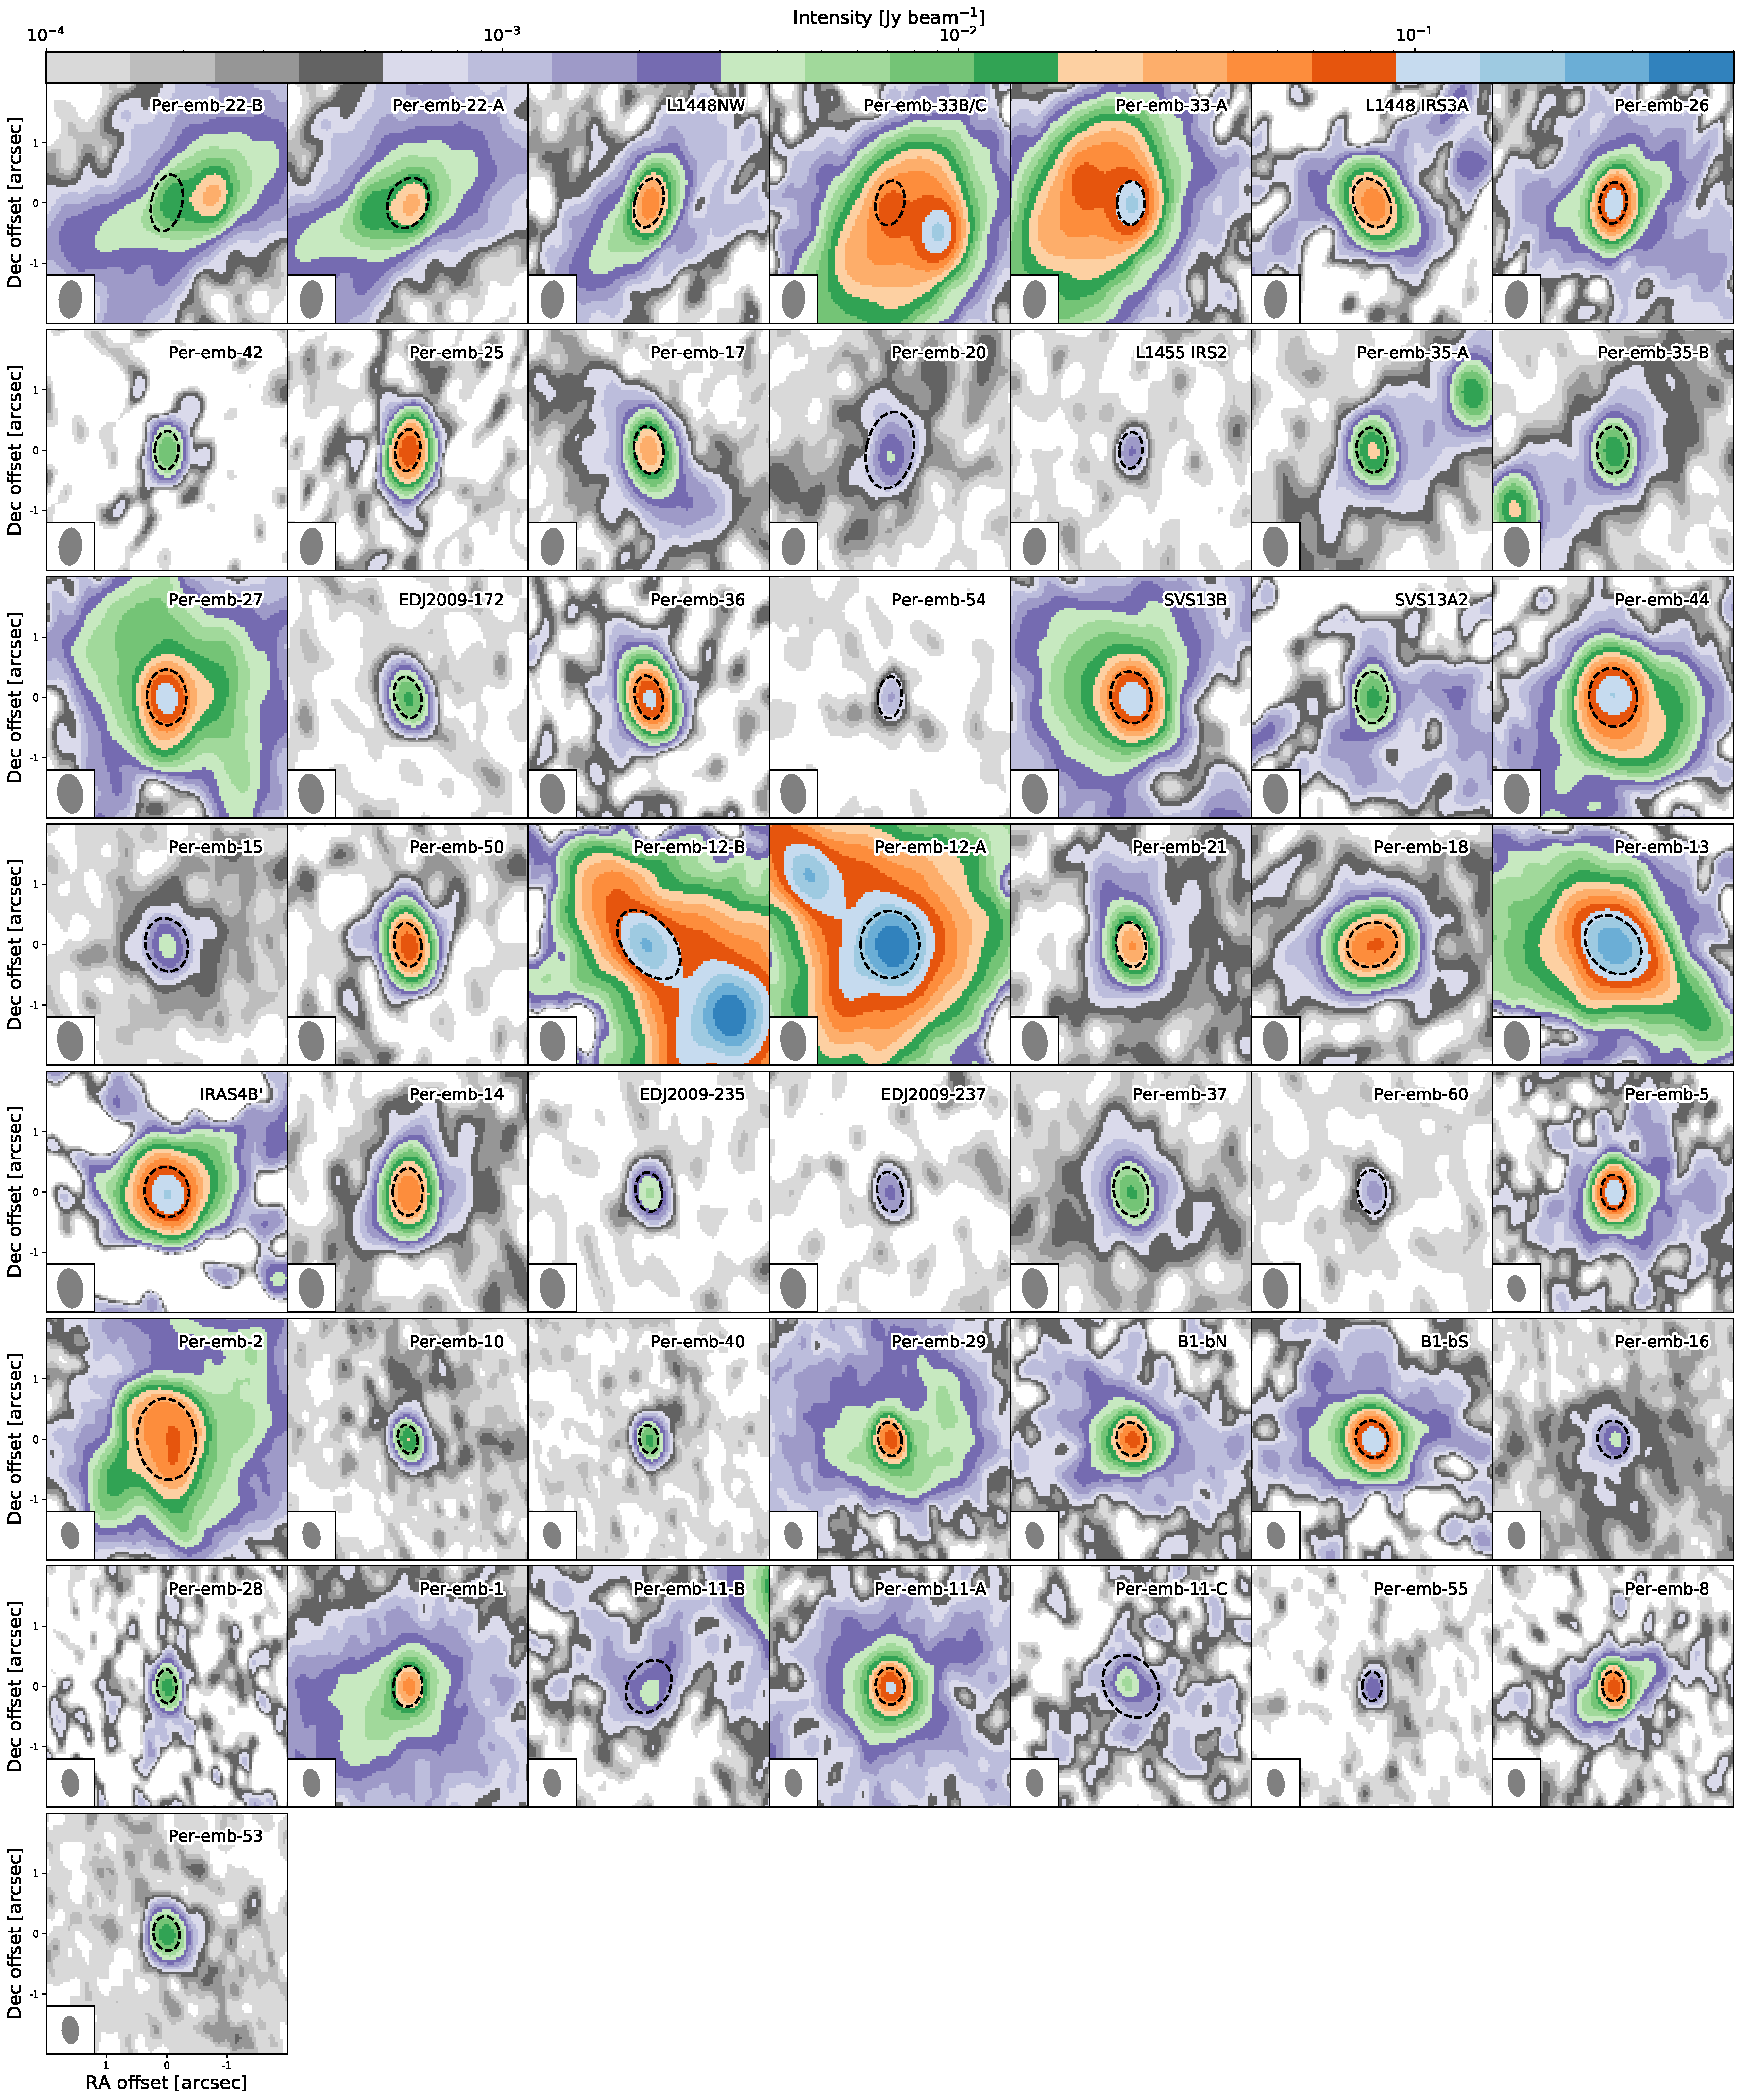
\includegraphics[width=\textwidth]{all_continuum.pdf}
  \caption{The continuum images of all PEACHES protostars.  Non-detections toward L1448 IRS\,2E and NGC 1333 SVS 3 are not shown.  The dashed ellipses illustrate the size of fitted continuum, which is the region for extracting 1D spectra.}
  \label{fig:continuum}
\end{figure*}

\begin{figure*}[htbp!]
  \centering
  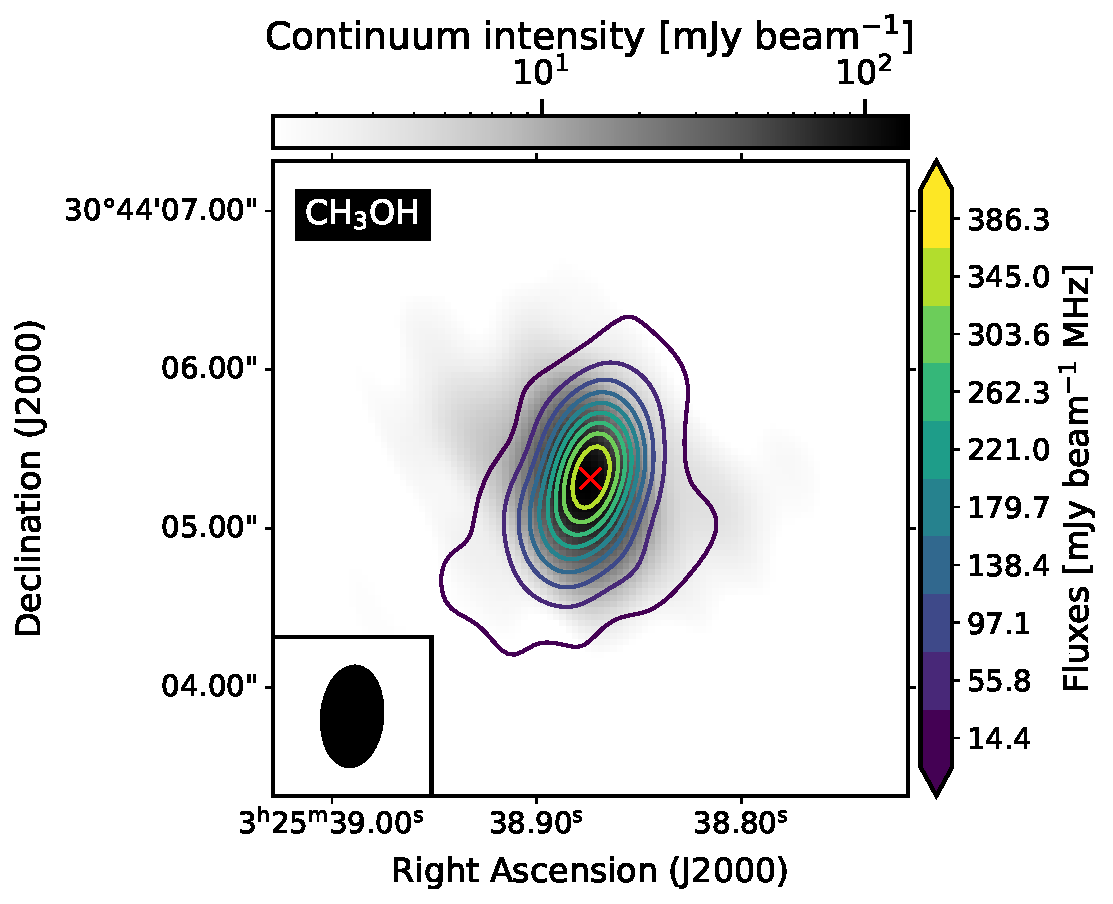
\includegraphics[width=0.24\textwidth]{Set1_ID02_CH3OH_243915.pdf}
  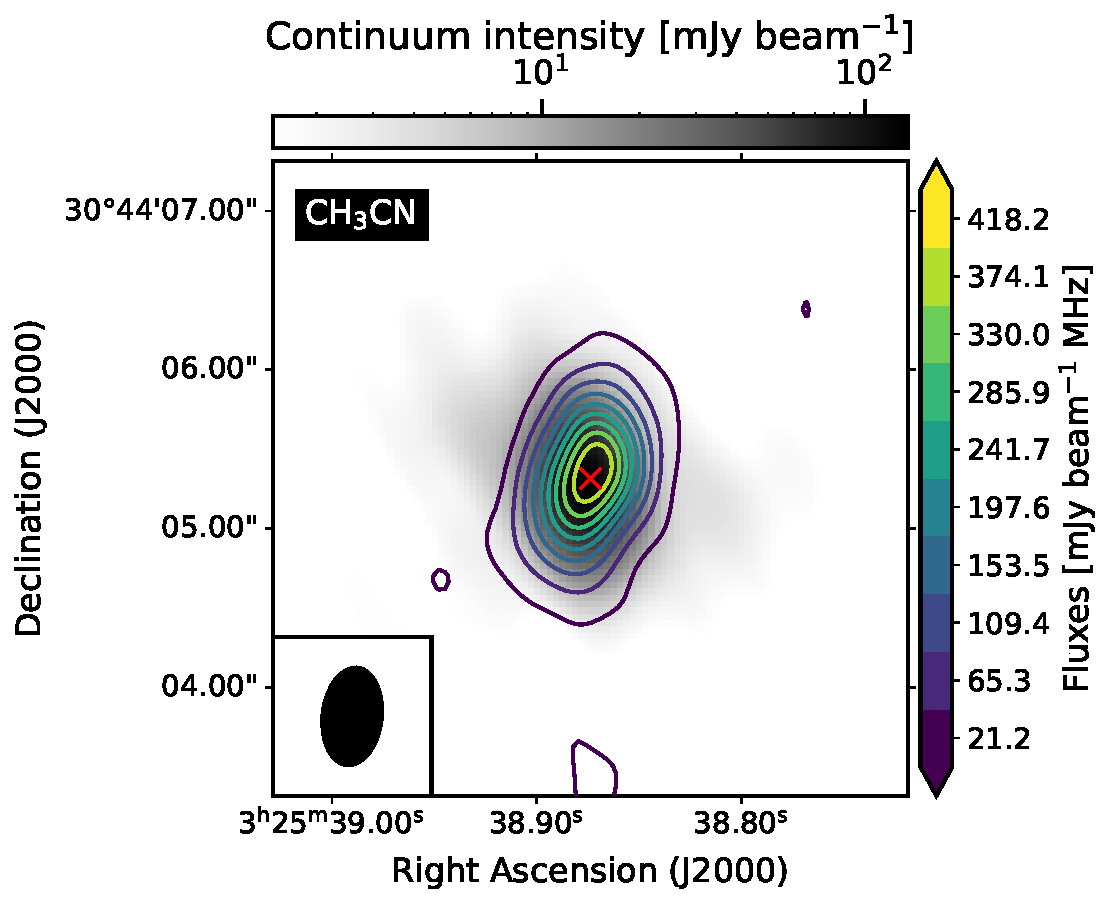
\includegraphics[width=0.24\textwidth]{Set1_ID02_CH3CN_257527.pdf}
  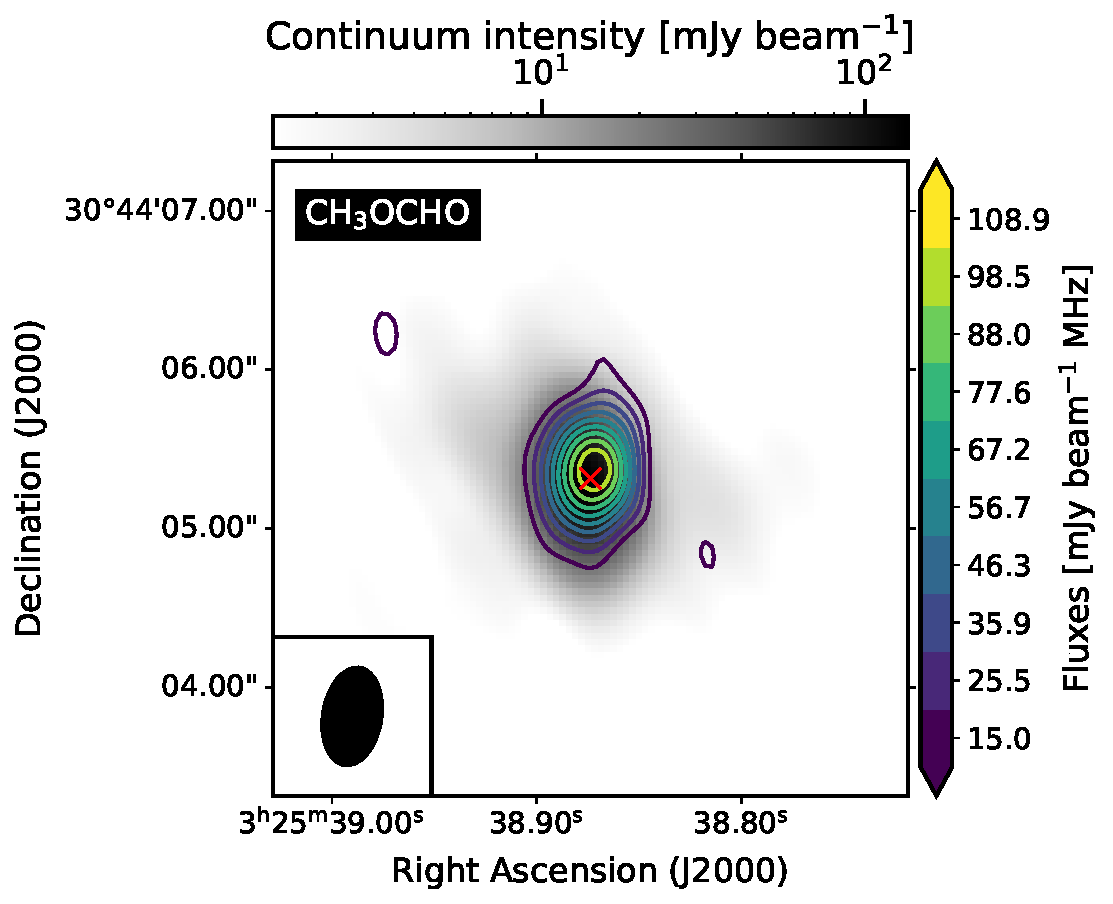
\includegraphics[width=0.24\textwidth]{Set1_ID02_CH3OCHO_259342.pdf}
  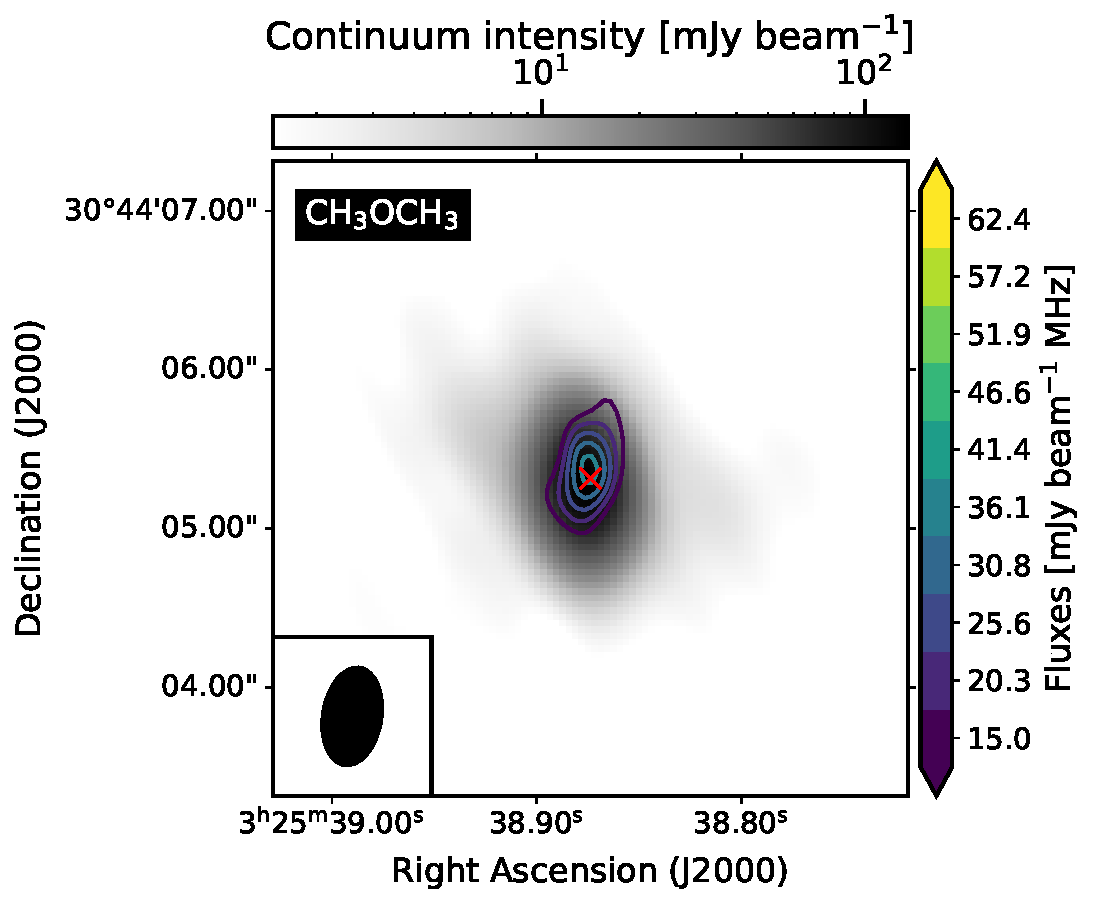
\includegraphics[width=0.24\textwidth]{Set1_ID02_CH3OCH3_259311.pdf}

  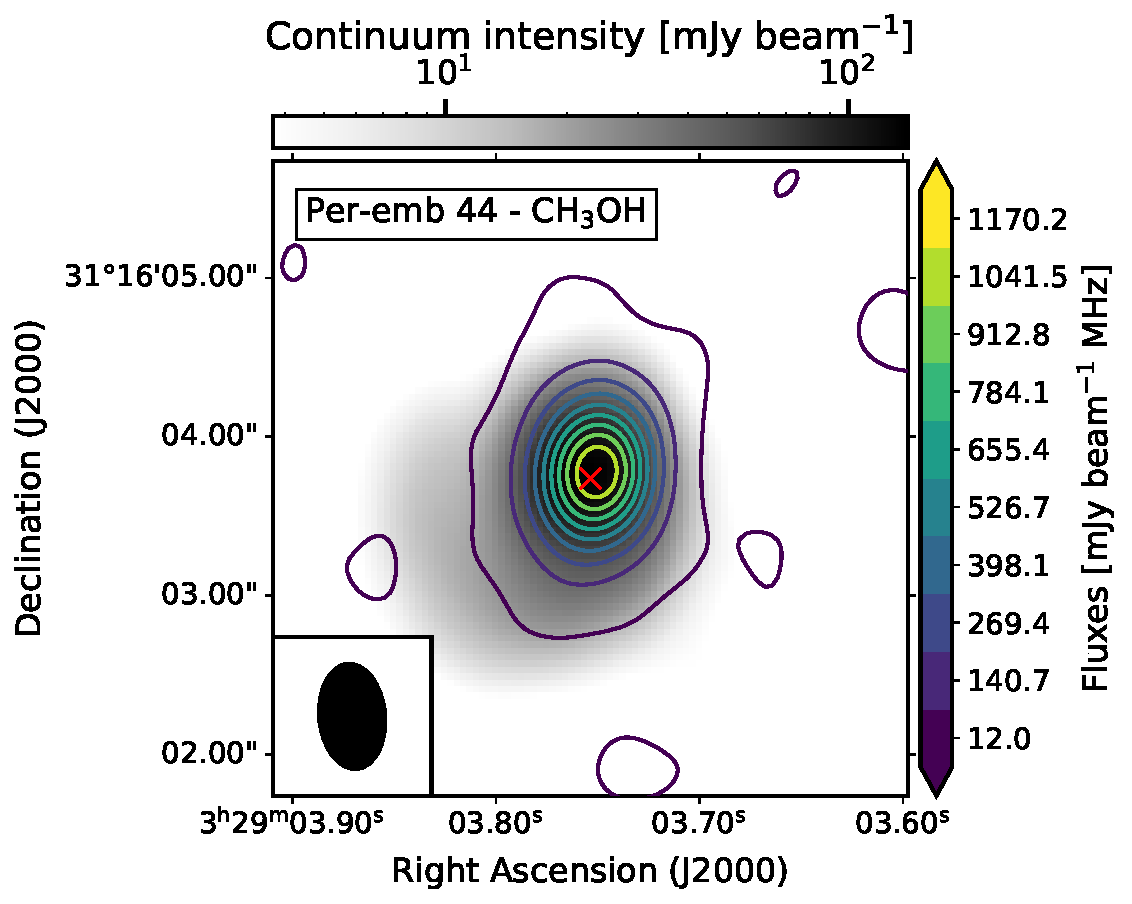
\includegraphics[width=0.24\textwidth]{Set2_ID00_CH3OH_243915.pdf}
  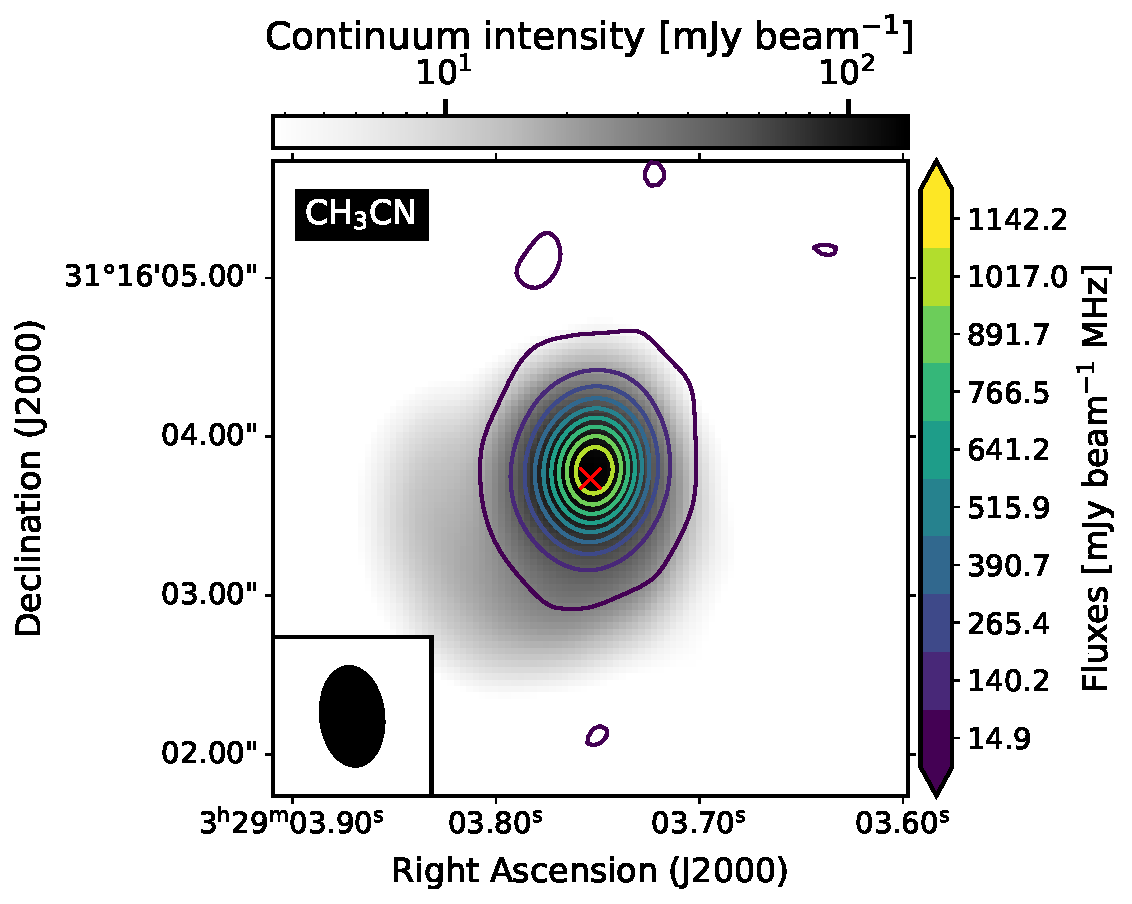
\includegraphics[width=0.24\textwidth]{Set2_ID00_CH3CN_257527.pdf}
  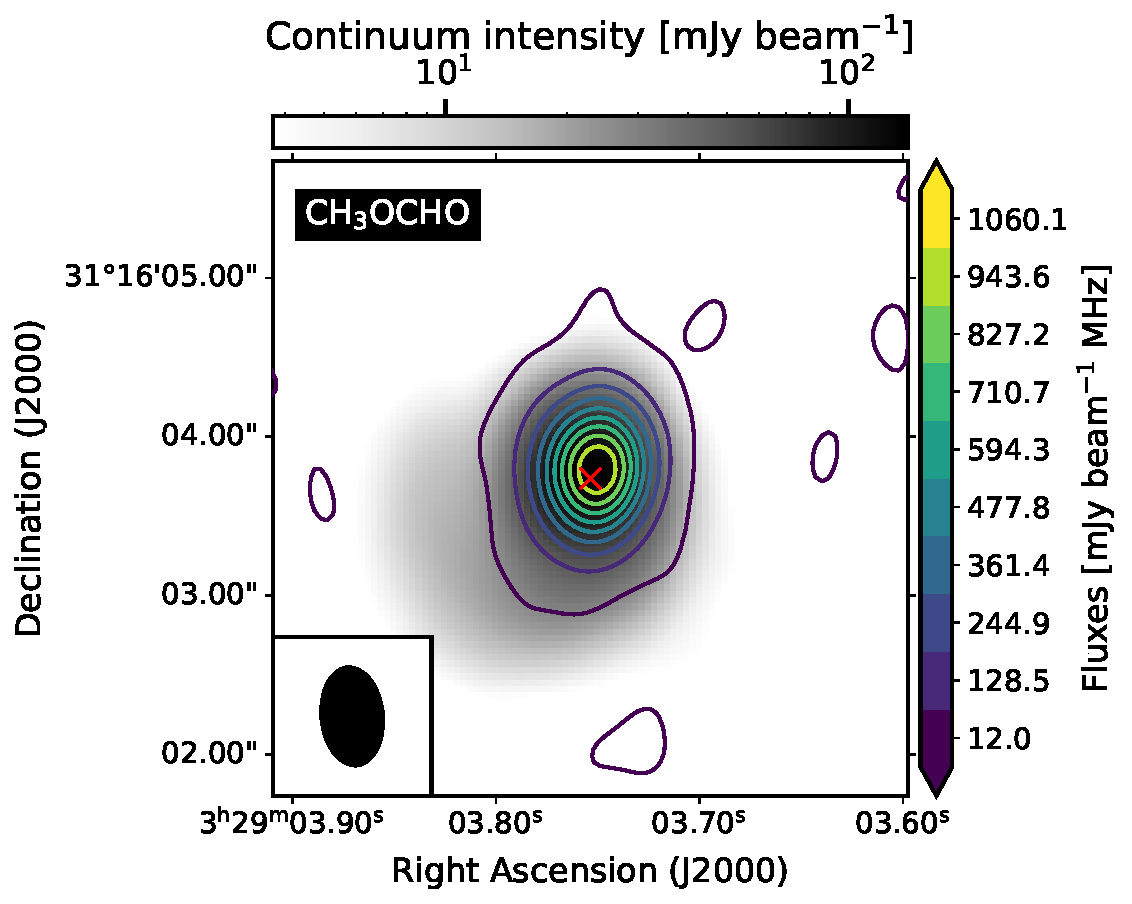
\includegraphics[width=0.24\textwidth]{Set2_ID00_CH3OCHO_259342.pdf}
  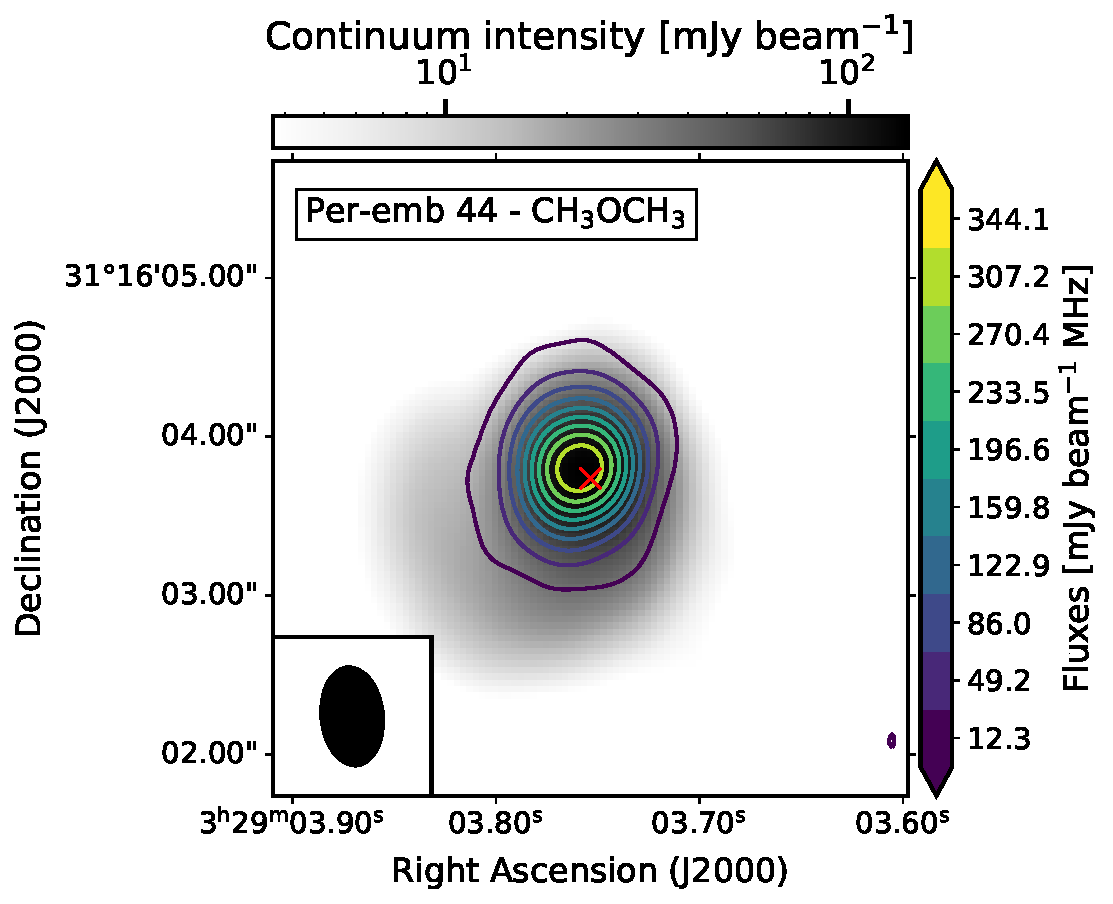
\includegraphics[width=0.24\textwidth]{Set2_ID00_CH3OCH3_259311.pdf}

  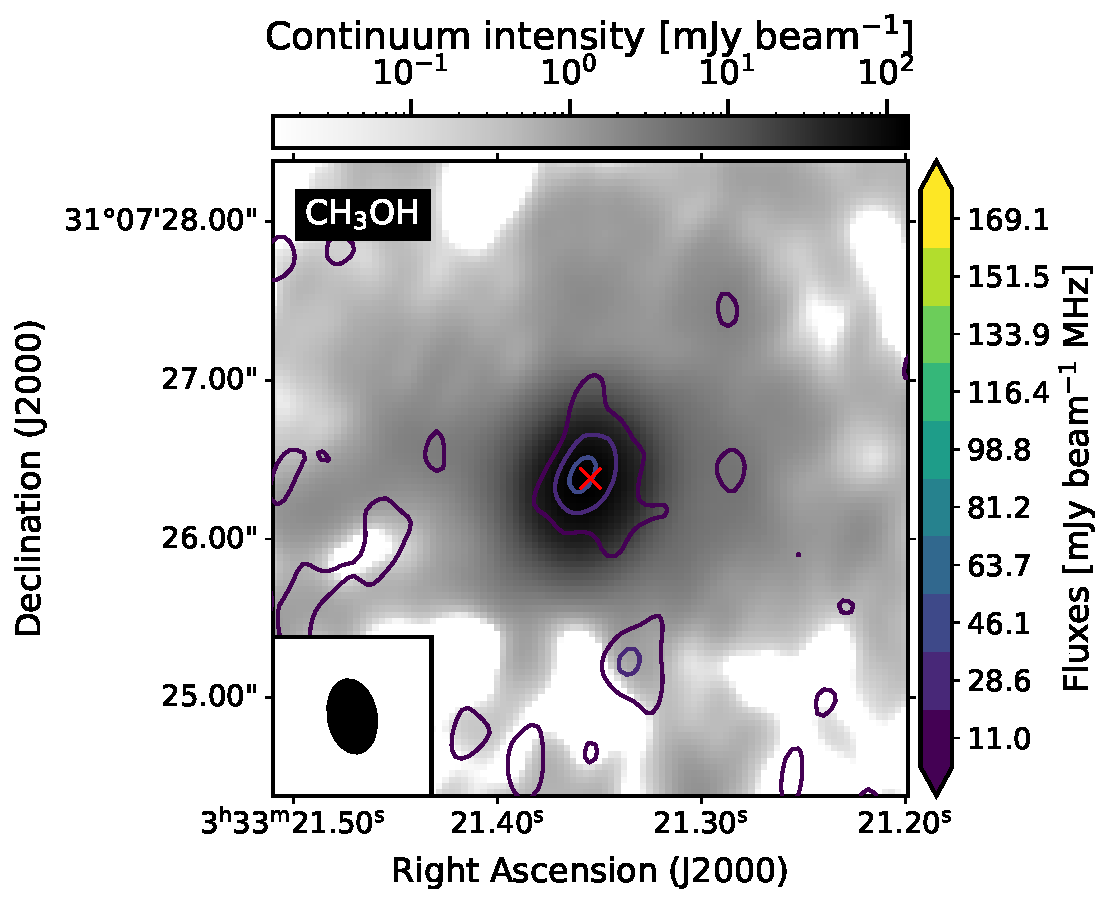
\includegraphics[width=0.24\textwidth]{Set3_ID00_CH3OH_243915.pdf}
  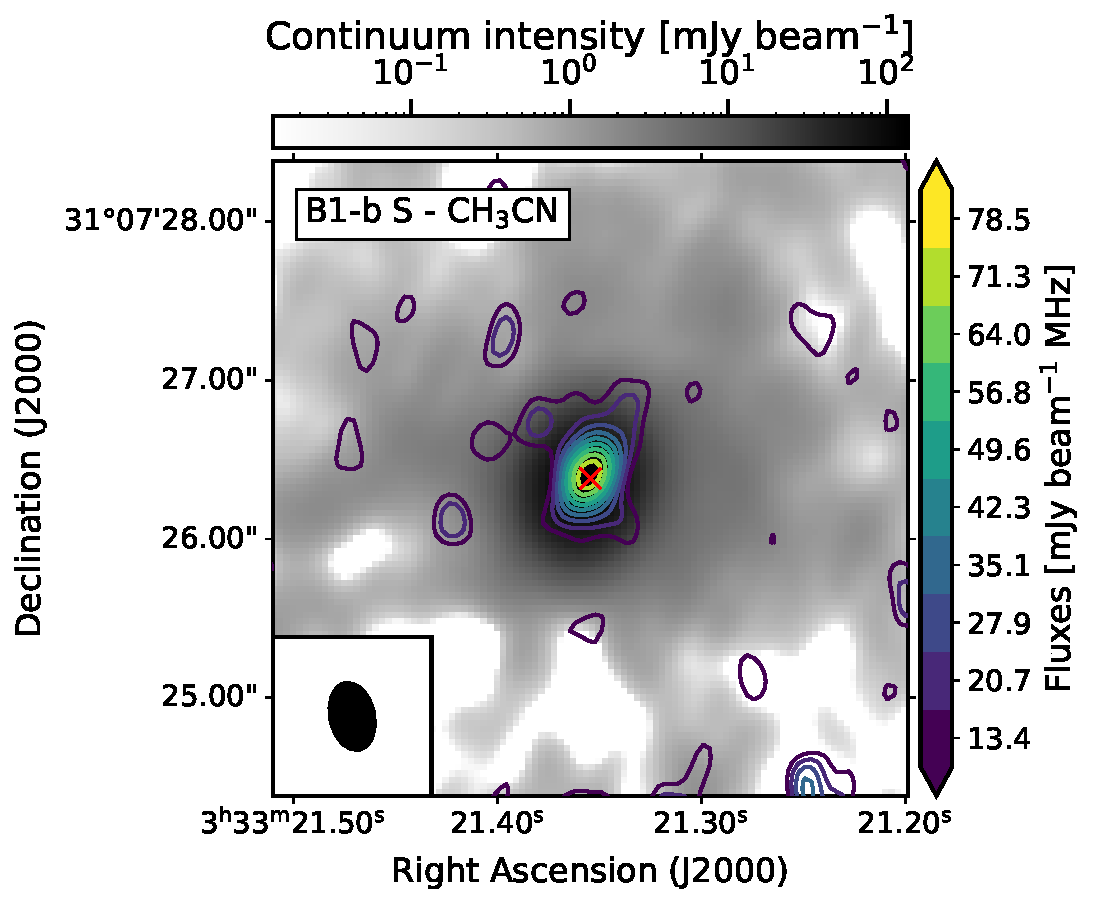
\includegraphics[width=0.24\textwidth]{Set3_ID00_CH3CN_257527.pdf}
  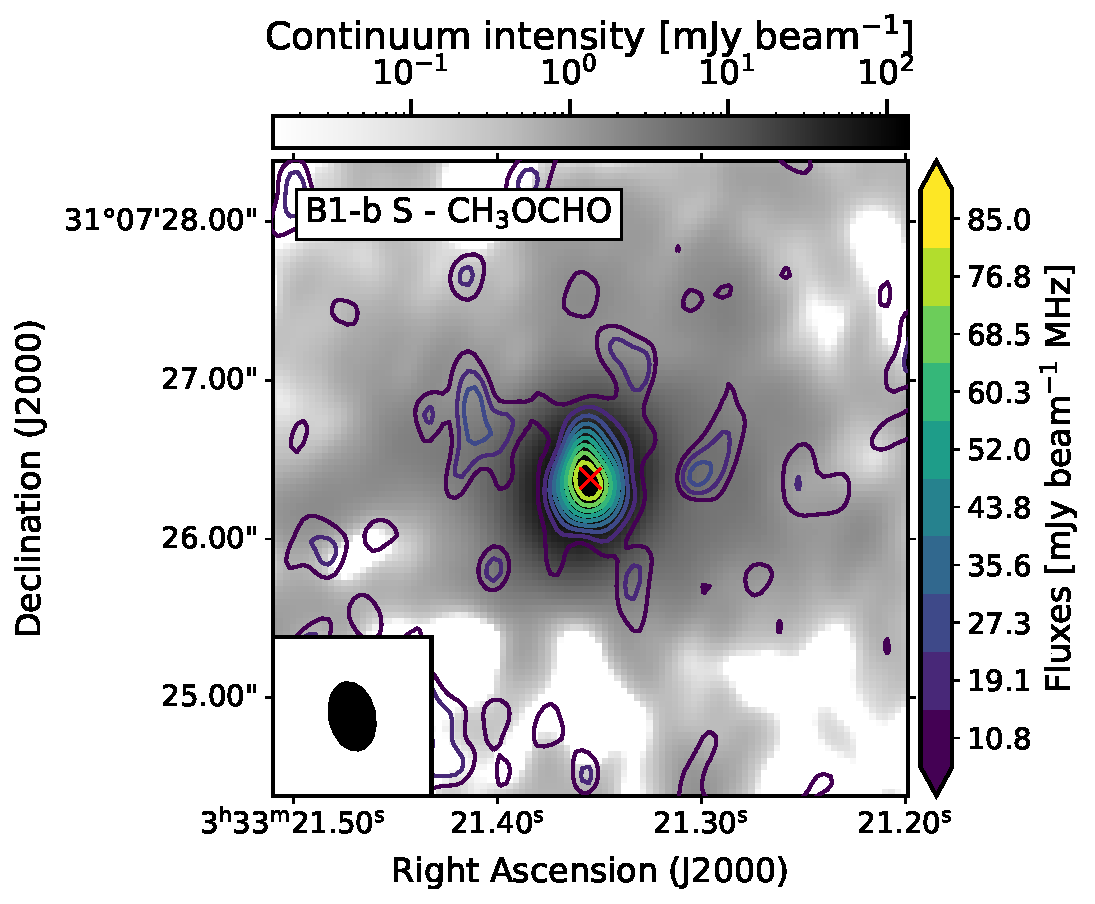
\includegraphics[width=0.24\textwidth]{Set3_ID00_CH3OCHO_259342.pdf}
  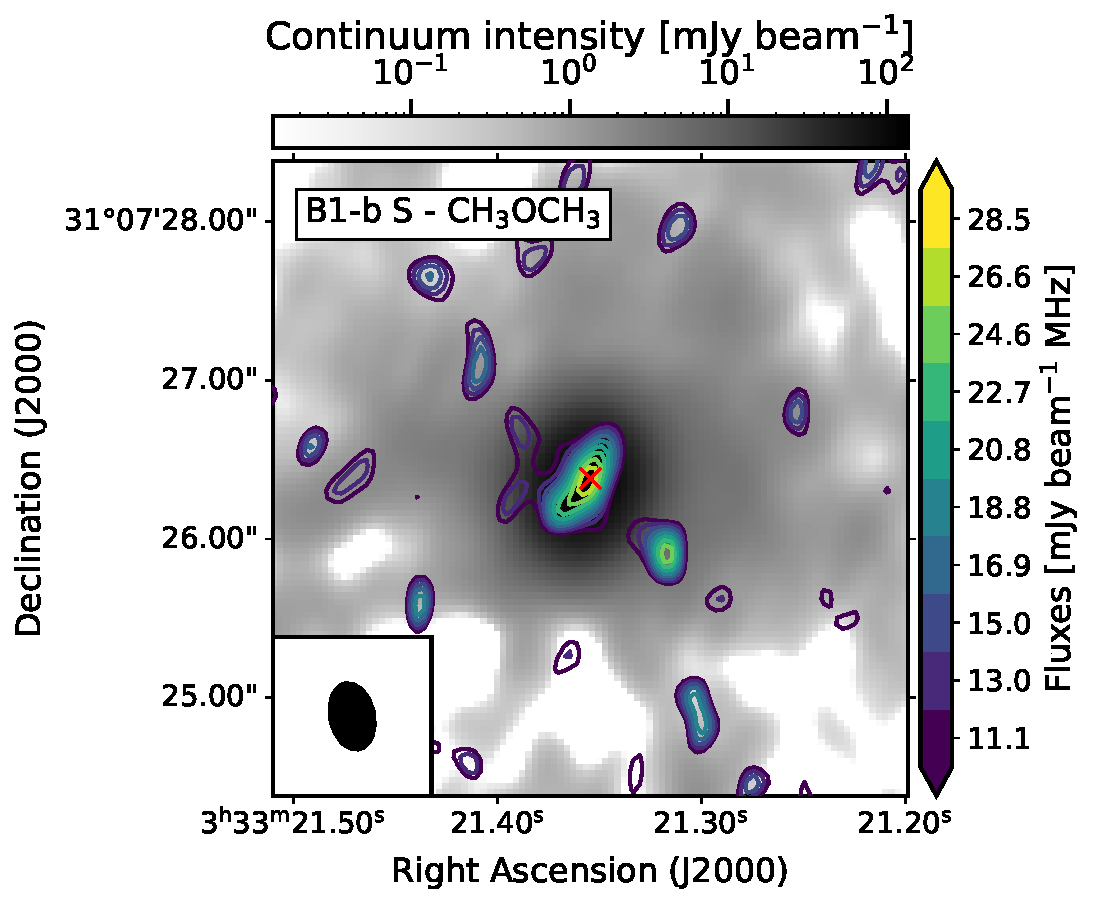
\includegraphics[width=0.24\textwidth]{Set3_ID00_CH3OCH3_259311.pdf}

  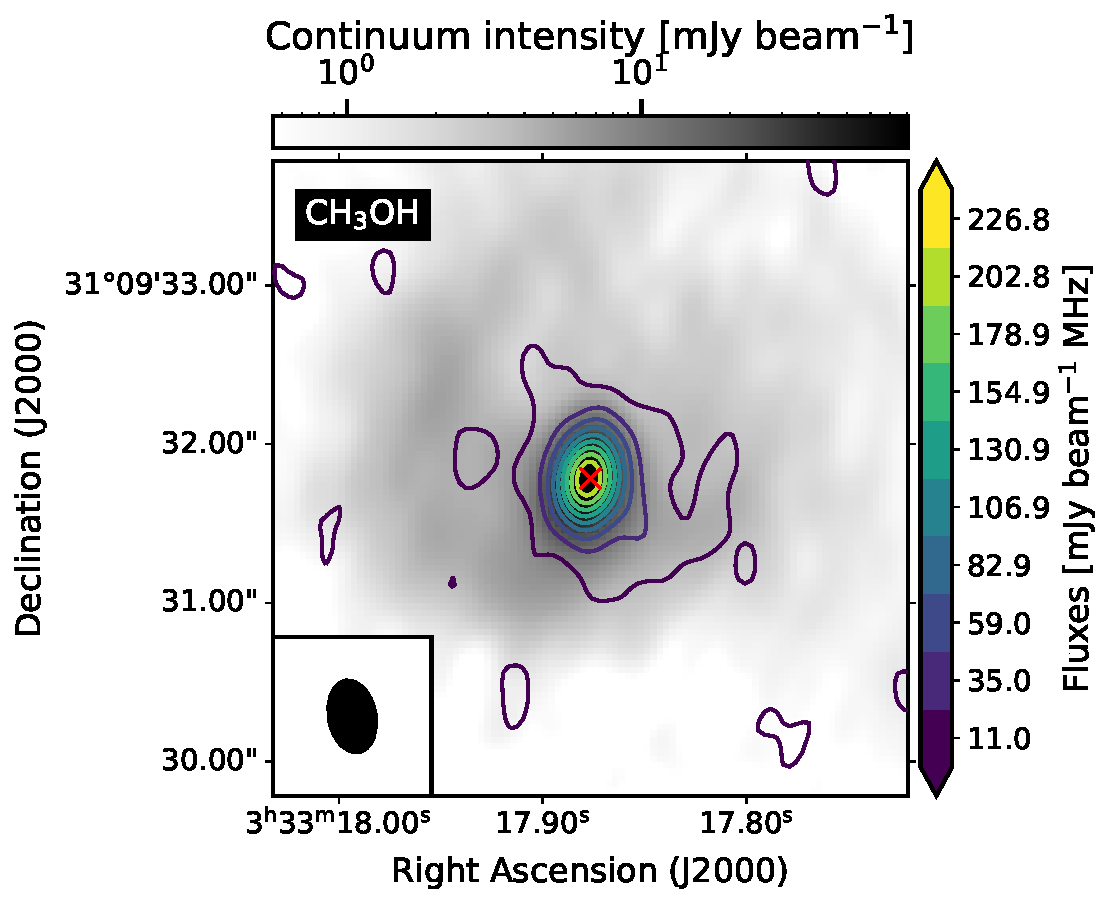
\includegraphics[width=0.24\textwidth]{Set3_ID01_CH3OH_243915.pdf}
  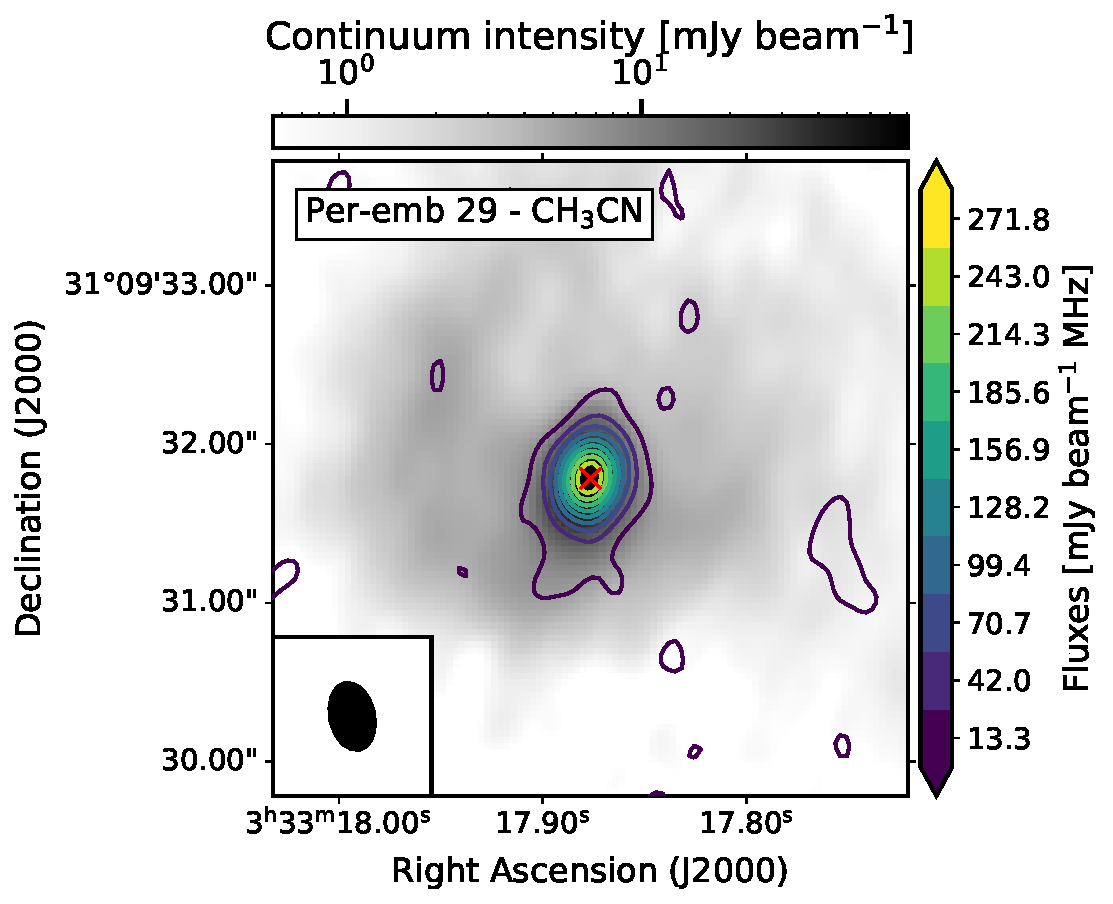
\includegraphics[width=0.24\textwidth]{Set3_ID01_CH3CN_257527.pdf}
  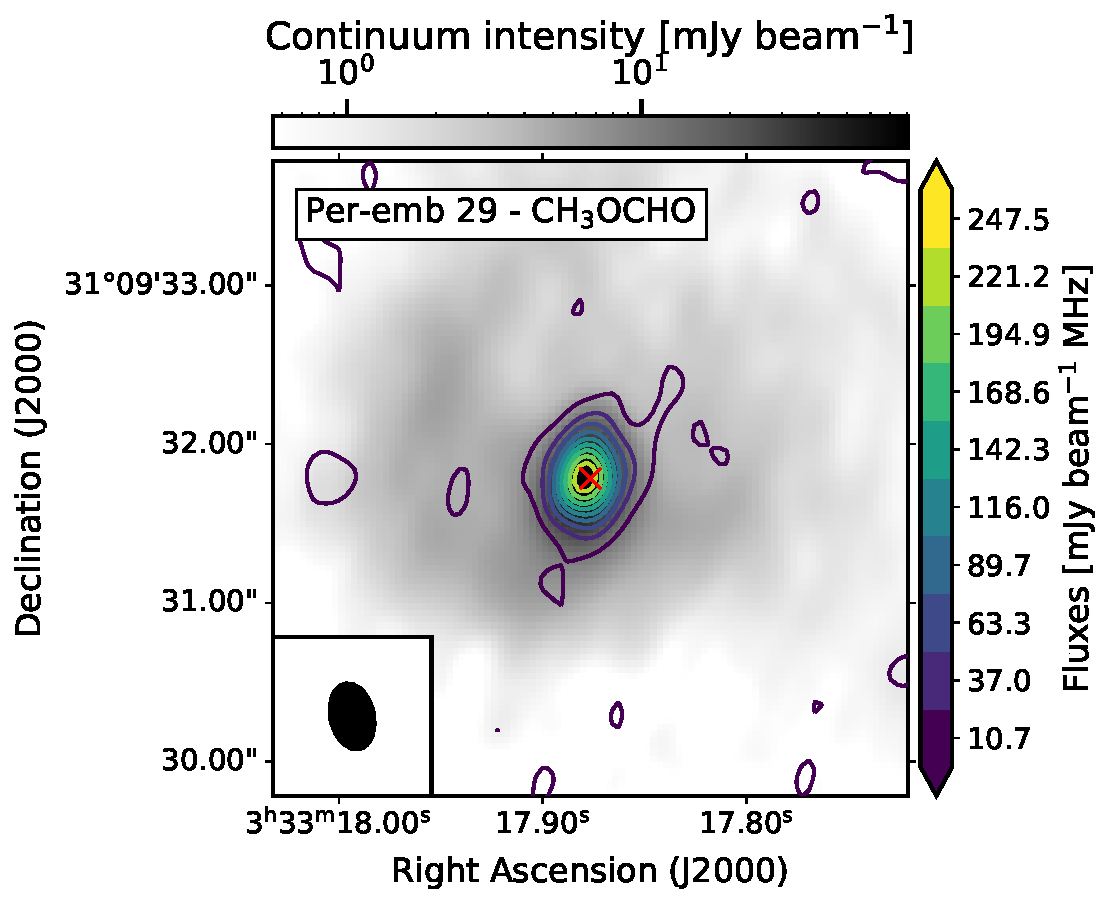
\includegraphics[width=0.24\textwidth]{Set3_ID01_CH3OCHO_259342.pdf}
  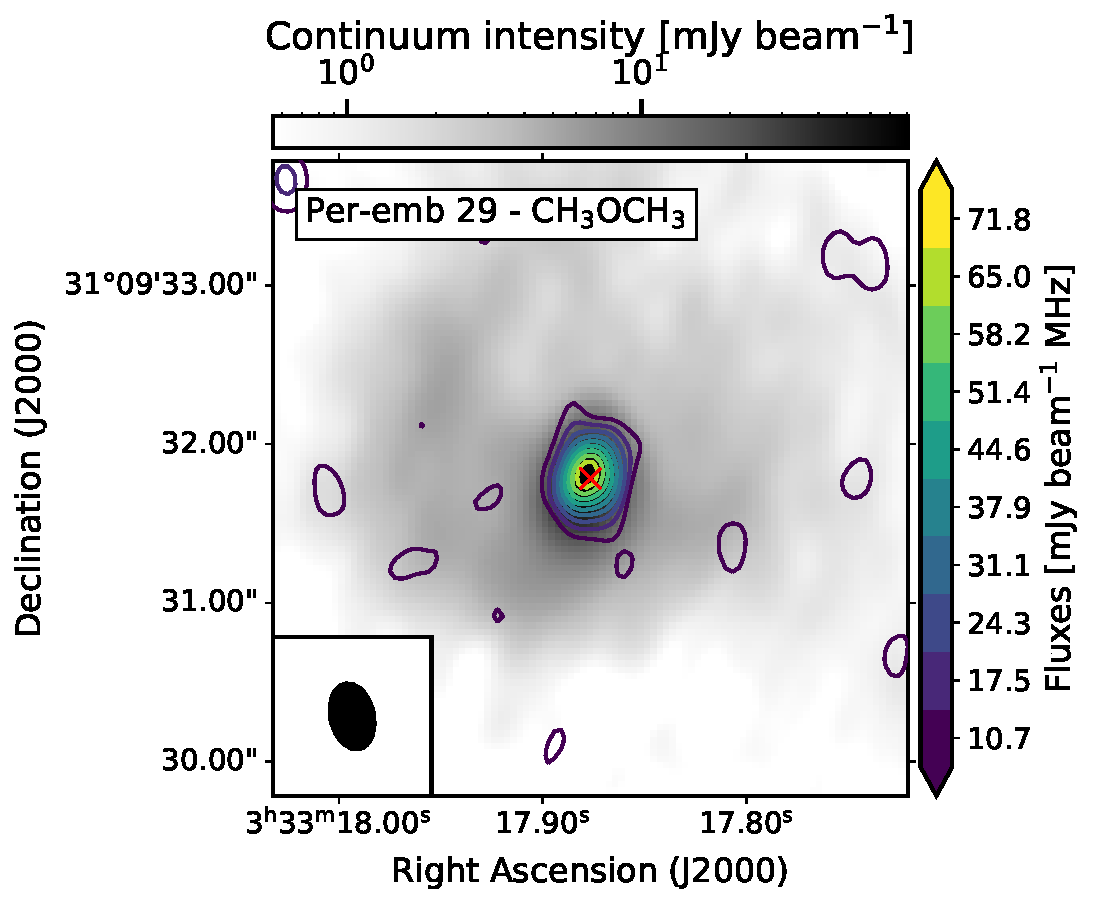
\includegraphics[width=0.24\textwidth]{Set3_ID01_CH3OCH3_259311.pdf}

  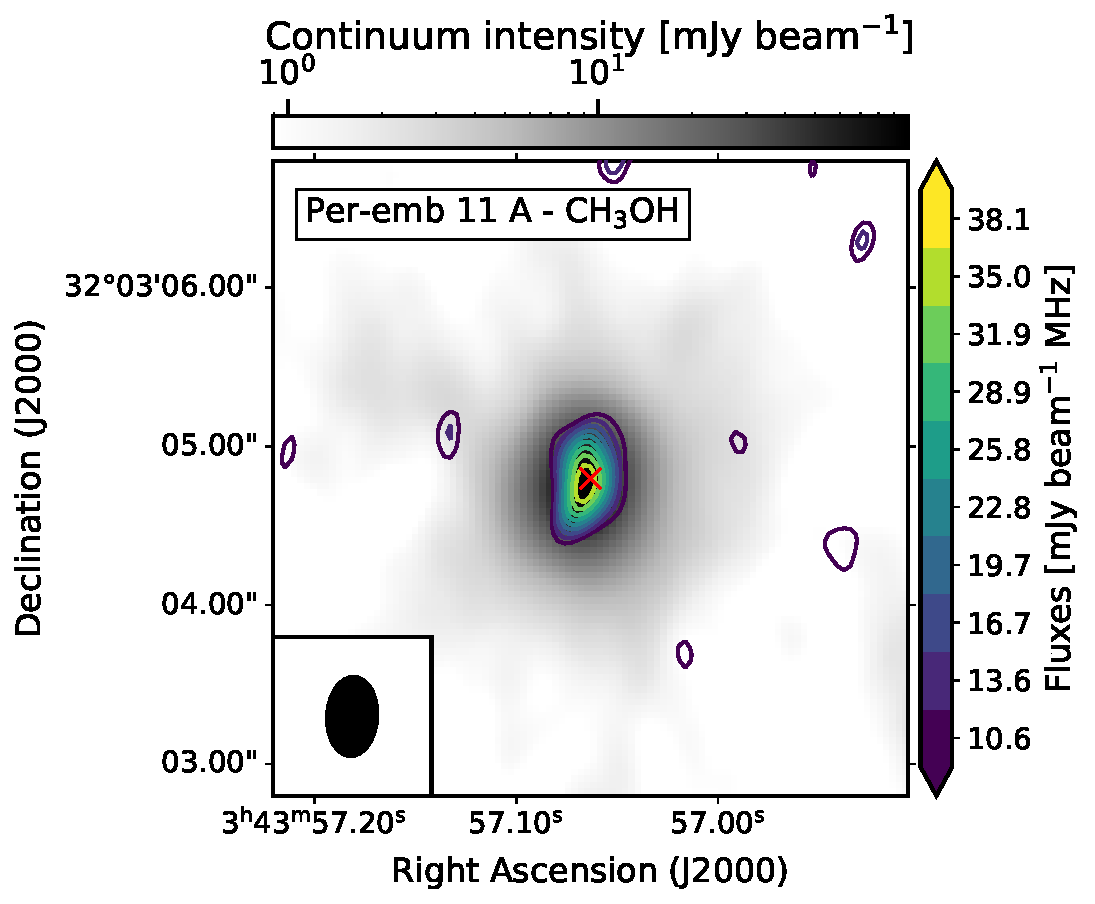
\includegraphics[width=0.24\textwidth]{Set3_ID07_CH3OH_243915.pdf}
  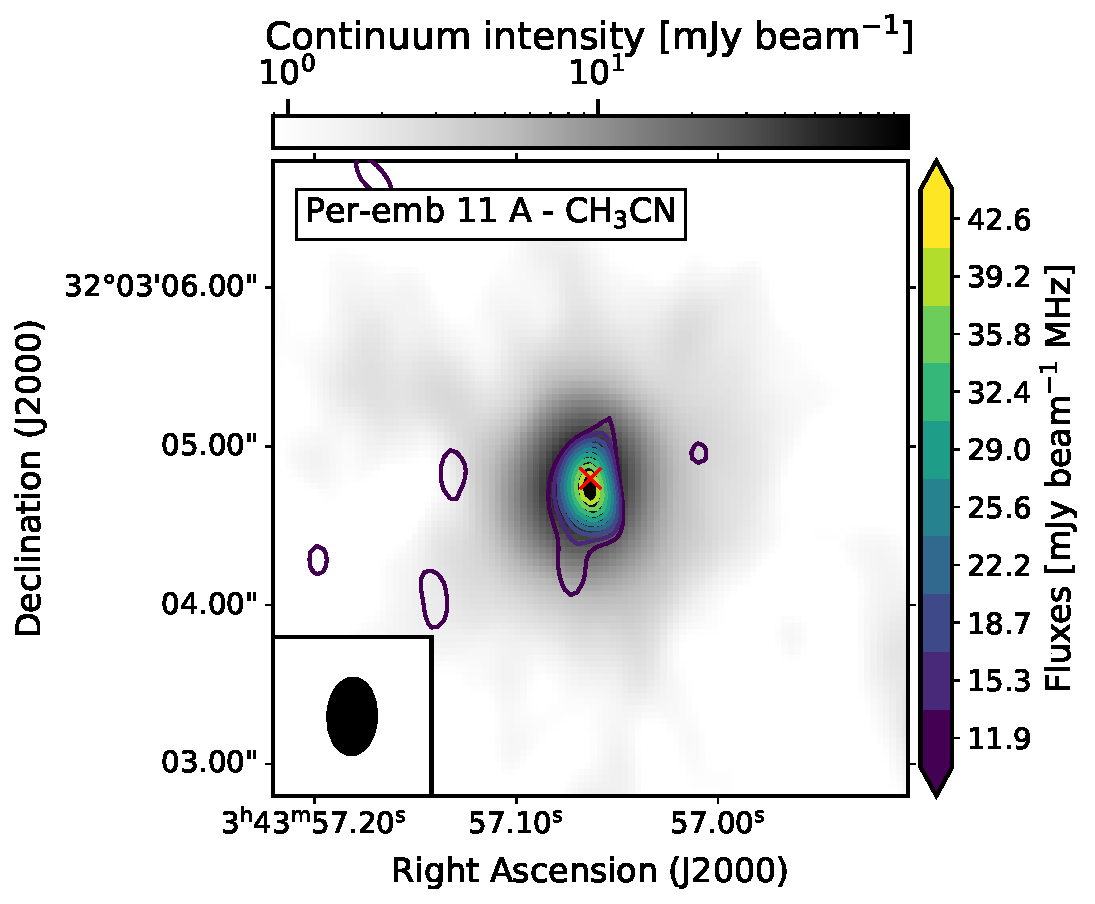
\includegraphics[width=0.24\textwidth]{Set3_ID07_CH3CN_257527.pdf}
  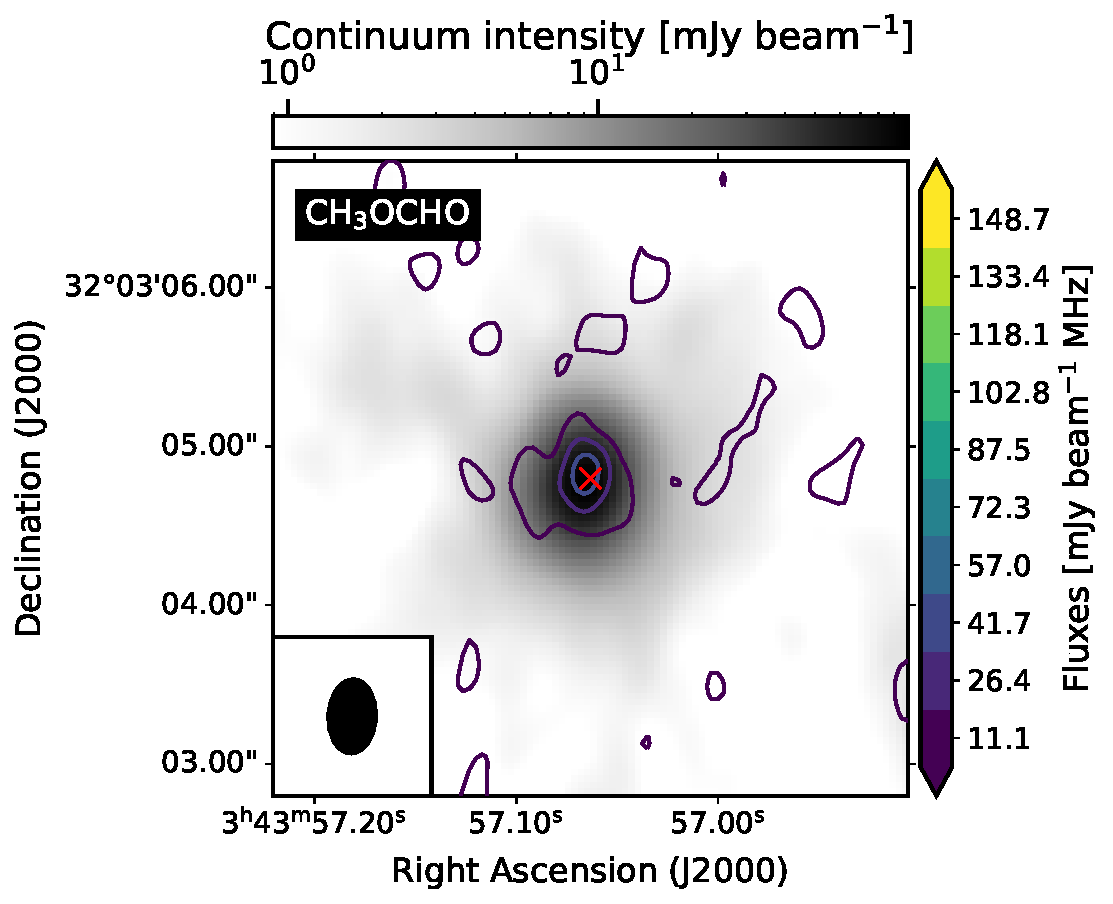
\includegraphics[width=0.24\textwidth]{Set3_ID07_CH3OCHO_259342.pdf}
  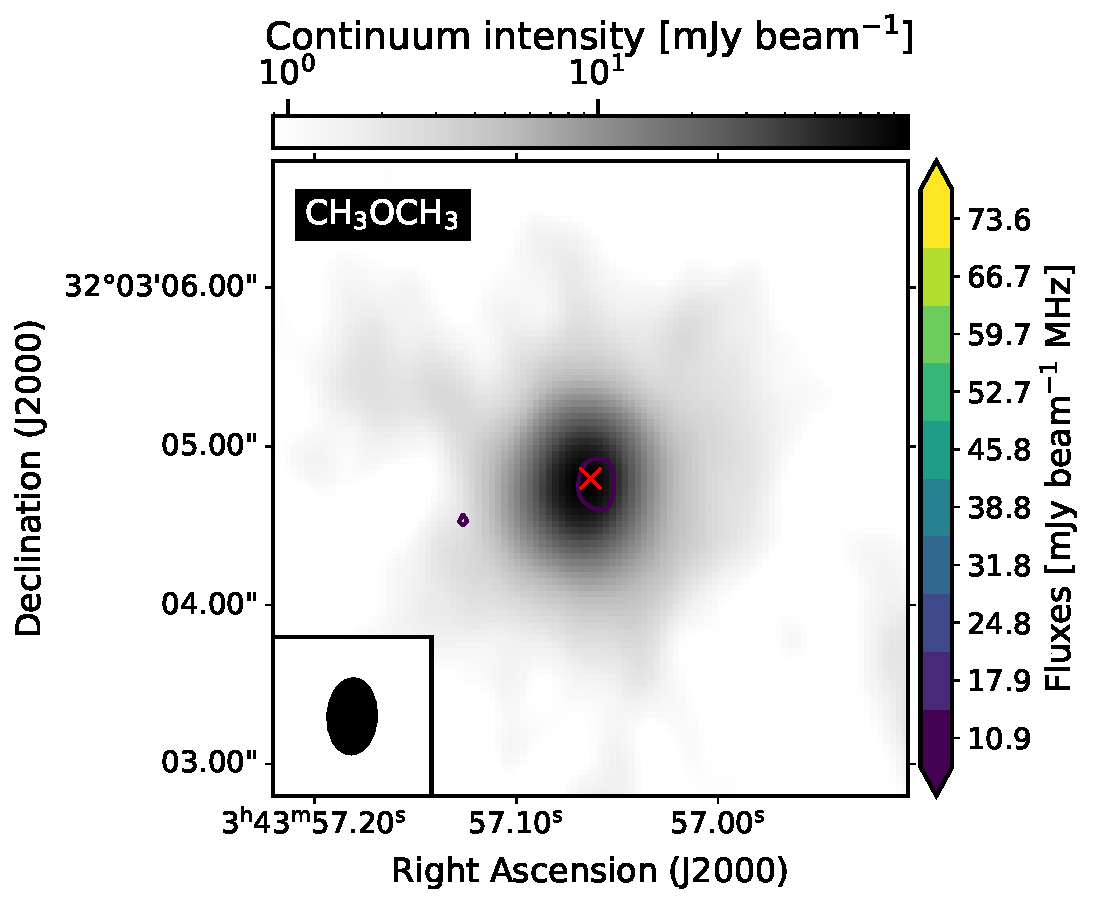
\includegraphics[width=0.24\textwidth]{Set3_ID07_CH3OCH3_259311.pdf}

  \caption{The intensity maps of most detected COMs, \methanol, \methylcyanide, \methylformate, and \dimethylether\ (from left to right).  Each row shows the emission from Per-emb 26, Per-emb 44, B1-b S, B1-c, and Per-emb 11 A (top to bottom).  The intensity is calculated by integrating over 3\kms\ around the line centroid, while the lowest contour shows the 3$\sigma$ value.  The grayscale images illustrate the continuum emission.}
  \label{fig:coms_map_sample}
\end{figure*}

\subsection{Line Identification and Modeling}
\label{sec:modeling}
Line identification starts with manual identification and verification for a few sources with rich spectra, including Per-emb-12B and B1-bS.  We use \textsc{splatalogue}\footnote{\href{http://www.splatalogue.net/}{http://www.splatalogue.net/}} to identity the molecular species and use \textsc{xclass} \citep{2017A&A...598A...7M} to verify the identification.  The \textsc{xclass} package is a LTE radiative transfer code that uses the molecular data from the Cologne Database of Molecular Spectroscopy (CDMS; \citealt{2001A&A...370L..49M,2005JMoSt.742..215M,2016JMoSp.327...95E}) and the Jet Propulsion Laboratory (JPL; \citealt{1998JQSRT..60..883P}).  An identification needs to satisfy the following criteria.
\begin{itemize}
  \item The spectra agree with the predicted strengths of the model.
  \item The spectral lines are not all blended with other emission, such as other molecules and the SiO emission tracing the outflows.  The emission of a few species, such as HDCO \&\ \tmethanol, \methanol\ \&\ \methylformate, \acetaldehyde\ \&\ \dmethanol, $^{34}$SO \&\ \ethanol, and \dimethylether\ \&\ \dmethylcyanide, are partially blended (blending occurs at a few lines but other lines remain isolated).  The fittings of those species are performed together to verify their identification.
  \item Identified molecules need to be already found toward young stellar objects as summarized in \citet{2018ApJS..239...17M}.
\end{itemize}
Table\,\ref{tbl:line_id} lists the identified species and transitions that are detected in at least one of the PEACHES protostars.  Only identifiable transitions are listed.  The \textsc{xclass} modeling include all the transitions in our frequency coverage for each molecule regardless their Einstein-A values and upper energy levels.  

As shown in Figure\,\ref{fig:coms_map_sample}, COMs emission centers around the protostars at $\sim 100-200$\,au.  At the similar region, the gas density is around $\sim 10^{8}$\cc\ \citep[B1-b S: ][]{2017A&A...606A..35G}, similar to the critical density of the COM emission detected in our observations.  For example, the \methanol\ line at 243915\mhz\ has a critical density of 1.4\ee{8}\cc\ \citep{2005A&A...432..369S,2010MNRAS.406...95R}.  Thus, the assumption of LTE holds for modeling the COM emission.  \textcolor{red}{YLY: B1-b S is one of the most dense protostars.  My guess is that the COMs is close to LTE but not in LTE.  We also test the LTE assumption on \methanol\ with the large velocity gradient (LVG) model using RADEX (\refnote).  The column density difference is only X\%.}

Systematic spectral fitting using \textsc{xclass} is applied to all sources using a list of species, compiled from the identifications.  Appendix\,\ref{sec:catalogs} lists the catalogs used in this study.  The fitting function in \textsc{xclass} includes several optimization algorithms that can be used in series to reduce biases.  We configure the algorithm chain that starts with the genetic algorithm followed by the Levenberg-Marquardt $\chi^{2}$ minimization.  The genetic algorithm searches the best-fitting parameters iteratively with generations that evolve like a natural selection, where the better fitting models get less modification over generations.  We setup the genetic algorithm to search for the top two best-fitting models with 30 generations.  Then, the Levenberg-Marquardt $\chi^{2}$ minimization applies to the two best-fitting models for 20 iterations to find the best-fitting models.  The genetic algorithm aims to find local minimums and the Levenberg-Marquardt minimization further finds the best-fitting models in the local minimums.  The two best-fitting models found by the genetic algorithm often very similar, suggesting that there is only one minimum.  To address the rare cases of two separated local minimums, we pick the model with the lower $\chi^{2}$ values from the two best-fitting models constrained by the Levenberg-Marquardt minimization.  

There are five parameters in the \textsc{xclass} modeling, the size of the emitting molecule ($r_\text{COM}$), the excitation temperature ($T_\text{ex}$), the column density ($N_\text{COM}$), the line width ($\Delta \nu$), and velocity offset ($v_\text{off}$).  We assume the COMs are all concentrated at the center, simplified as a 2D thin circular disk.  We fix $r_\text{COM}$ as 0\farcs{5}, similar to our beam size, and optimize the model with five excitation temperatures, 100, 150, 200, 250, and 300 K.  We allow the line width varying between 1.2\kms\ to 3.5\kms\ for better fitting quality but assume no velocity offset from the source velocity, and the allowed range of the column density for each molecule is chosen according to the strength of the emission.  From the fitting results of five $T_\text{ex}$, if a molecule is detected, the mean column densities will be the best-fitting column density, while the range of the column densities indicates the upper and lower uncertainties.  If a molecule is non-detection, the synthetic spectra for all lines are scaled to match the peaks of the each line fitted by a Gaussian profile.  Then, we take the minimum of the corresponding column densities as the upper limit.

\section{Results}
\subsection{Detection Statistics}
We summarize the detection statistics in Figure\,\ref{fig:stats}, which includes COMs, the carbon-chain molecules, and the simple organic molecules, such as CS, \htcn, SO, $^{34}$SO, and SO$_{2}$.  In the following results of detection fraction, we include the three sources that are excluded from modeling due to no reliable source velocity, making a total of 50 sources.  The COMs discussed here are the derived from the spectra taken toward the continuum peak (Section\,\ref{sec:continuum}).  We focus on the chemistry of COMs in the disk-forming regions in this study, therefore, excluding detection of molecules outside the continuum peak.  A comparison of chemical composition in protostellar envelopes (100--1000\,au) requires observations with larger maximum recoverable scale ($\theta_\text{MRS}$).

The PEACHES protostars show a great chemical diversity from no molecule detected (e.g., B1-b N and L1455 IRS 2) to rich spectra of COMs (e.g., Per-emb 13).  Most of the PEACHES protostars have simple organics, such as SO, CS, \htcn, and HDCO, and $\sim 60$\%\ of sources have SO$_{2}$ and $^{34}$SO.  Emission of \cch\ can be easily identified from the spectra.  However, the \cch\ toward the continuum sources often shows irregular line profiles together with velocity offsets and absorption (Figure\,\ref{fig:all_cch}).  In fact, warm environments, such as the outflow cavity wall, easily enhance the abundance of \cch\ because of elevated abundance of C$^{+}$ \citep[e.g., ][]{2018ApJ...864...76Z,2019ApJ...873L..21I}.  Thus, \cch\ emission is extended along with the outflow cavities, making the 1D spectra toward the continuum source unrepresentative.  Observations with a larger $\theta_\text{MRS}$ will provide a complete representation of the \cch\ abundance on the inner envelope.

Several sources have their SiO emission with a broad line width, significantly contaminating the emission of \ethylcyanide\ and \acetaldehyde.  In the later quantitative discussion, we exclude the spectral windows contaminated by the SiO emission.  For assigning the detections, we can distinguish the emission of \ethylcyanide\ and \acetaldehyde\ from the broad SiO emission in a few sources, such as \acetaldehyde\ in Per-emb 26.

Figure\,\ref{fig:detection_summary} shows the number of COMs detected toward the PEACHES sample.  Twenty-one (45\%) sources have no COMs detected.  \methanol\ is detected in 28 sources (56\%); \methylformate\ is detected in 15 sources (32\%); and N-bearing COMs are detected in 20 sources (40\%).  Comparing to the COMs in the CALYPSO survey \citep{2020A&A...635A.198B}, the fraction of sources that have methanol, $\sim$50\%, is similar to that for the PEACHES protostars.  Also, 30\%\ of the CALYPSO sources have at least three COMs, while 28\%\ of the PEACHES protostars have at least three COMs.  

We compare the number of detected COMs with the bolometric luminosity (\lbol), the bolometric temperature (\tbol), and the dust mass estimated by \citet{2020arXiv200602812T} using observations at 9\,mm ($M_\text{central}$).  The number of COMs shows no obvious trend with \lbol, \tbol, and $M_\text{central}$.  For \lbol, the sources with at least three COMs all have \lbol\ $\gtrsim$ 3\msun, except for B1-b S.  However, the sources without any COMs also have a similar \lbol.  If COMs mostly come from thermal desorption, the region with $T > T_\text{desorption}$ may be smaller for the low luminosity sources, making the emission of COMs fainter and reducing our sensitivity to detect COMs.
The COM-rich sources have \tbol$\sim 50$\,K, while the COM-poor sources have a greater scatter of \tbol, ranging from 14.7\,K to 1100\,K.  The protostars with high $M_\text{central}$ ($>$666.5\mearth) have detections of COMs.  However, the protostars with low $M_\text{central}$ can have either many COMs or no COM.

The sources with high continuum brightness temperature (\tbc) tend to have rich spectra COMs (Figure\,\ref{fig:detection_summary_Tb}), while the sources with no detection of COM have their \tbc$\lesssim$10\,K.  The brightest source in continuum, Per-emb 12 A has many molecules detected in absorption due to the high continuum opacity blocking the emission of COMs \citep{2019ApJ...872..196S,2020ApJ...896L...3D}.  The continuum brightness temperature traces the gas column density, tracing the amount of embedding gas around the protostars.  
Thus, the tendency between many COMs and the high \tbc\ hints the scenarios where the denser envelope either increases the detectability of COMs or enhance the complexity of molecules.

% hot corino fraction and new hot corinos
Compact emission of COMs ($\sim$100--300\,au) suggests a warm temperature ($\gtrsim$100\,K) of COMs for a typical low-mass protostars \citep[e.g. ][]{2017ApJ...835..259Y}, consistent with an origin of thermal desorption at the inner envelope, so called hot corinos \citep{2004ASPC..323..195C}.  Only L1448 IRS 3A shows extended \methanol\ emission, and B1-b N shows no \methanol\ emission toward the continuum but peaks at $\sim$1\arcsec\ away from the continuum, hinting the existence of \methanol\ toward the continuum source blocked by opaque continuum \citep{2018A&A...620A..80M}.  Excluding L1448 IRS 3A, 28 sources (56\%) have hot corinos type chemistry.  Many of hot corinos are previously known (\refnote?), while our survey detects COMs other than \methanol\ toward Per-emb 35 A, Per-emb 35 B, Per-emb 11 A, Per-emb 11 C, and HH 211 MMS.

\begin{figure*}[htbp!]
  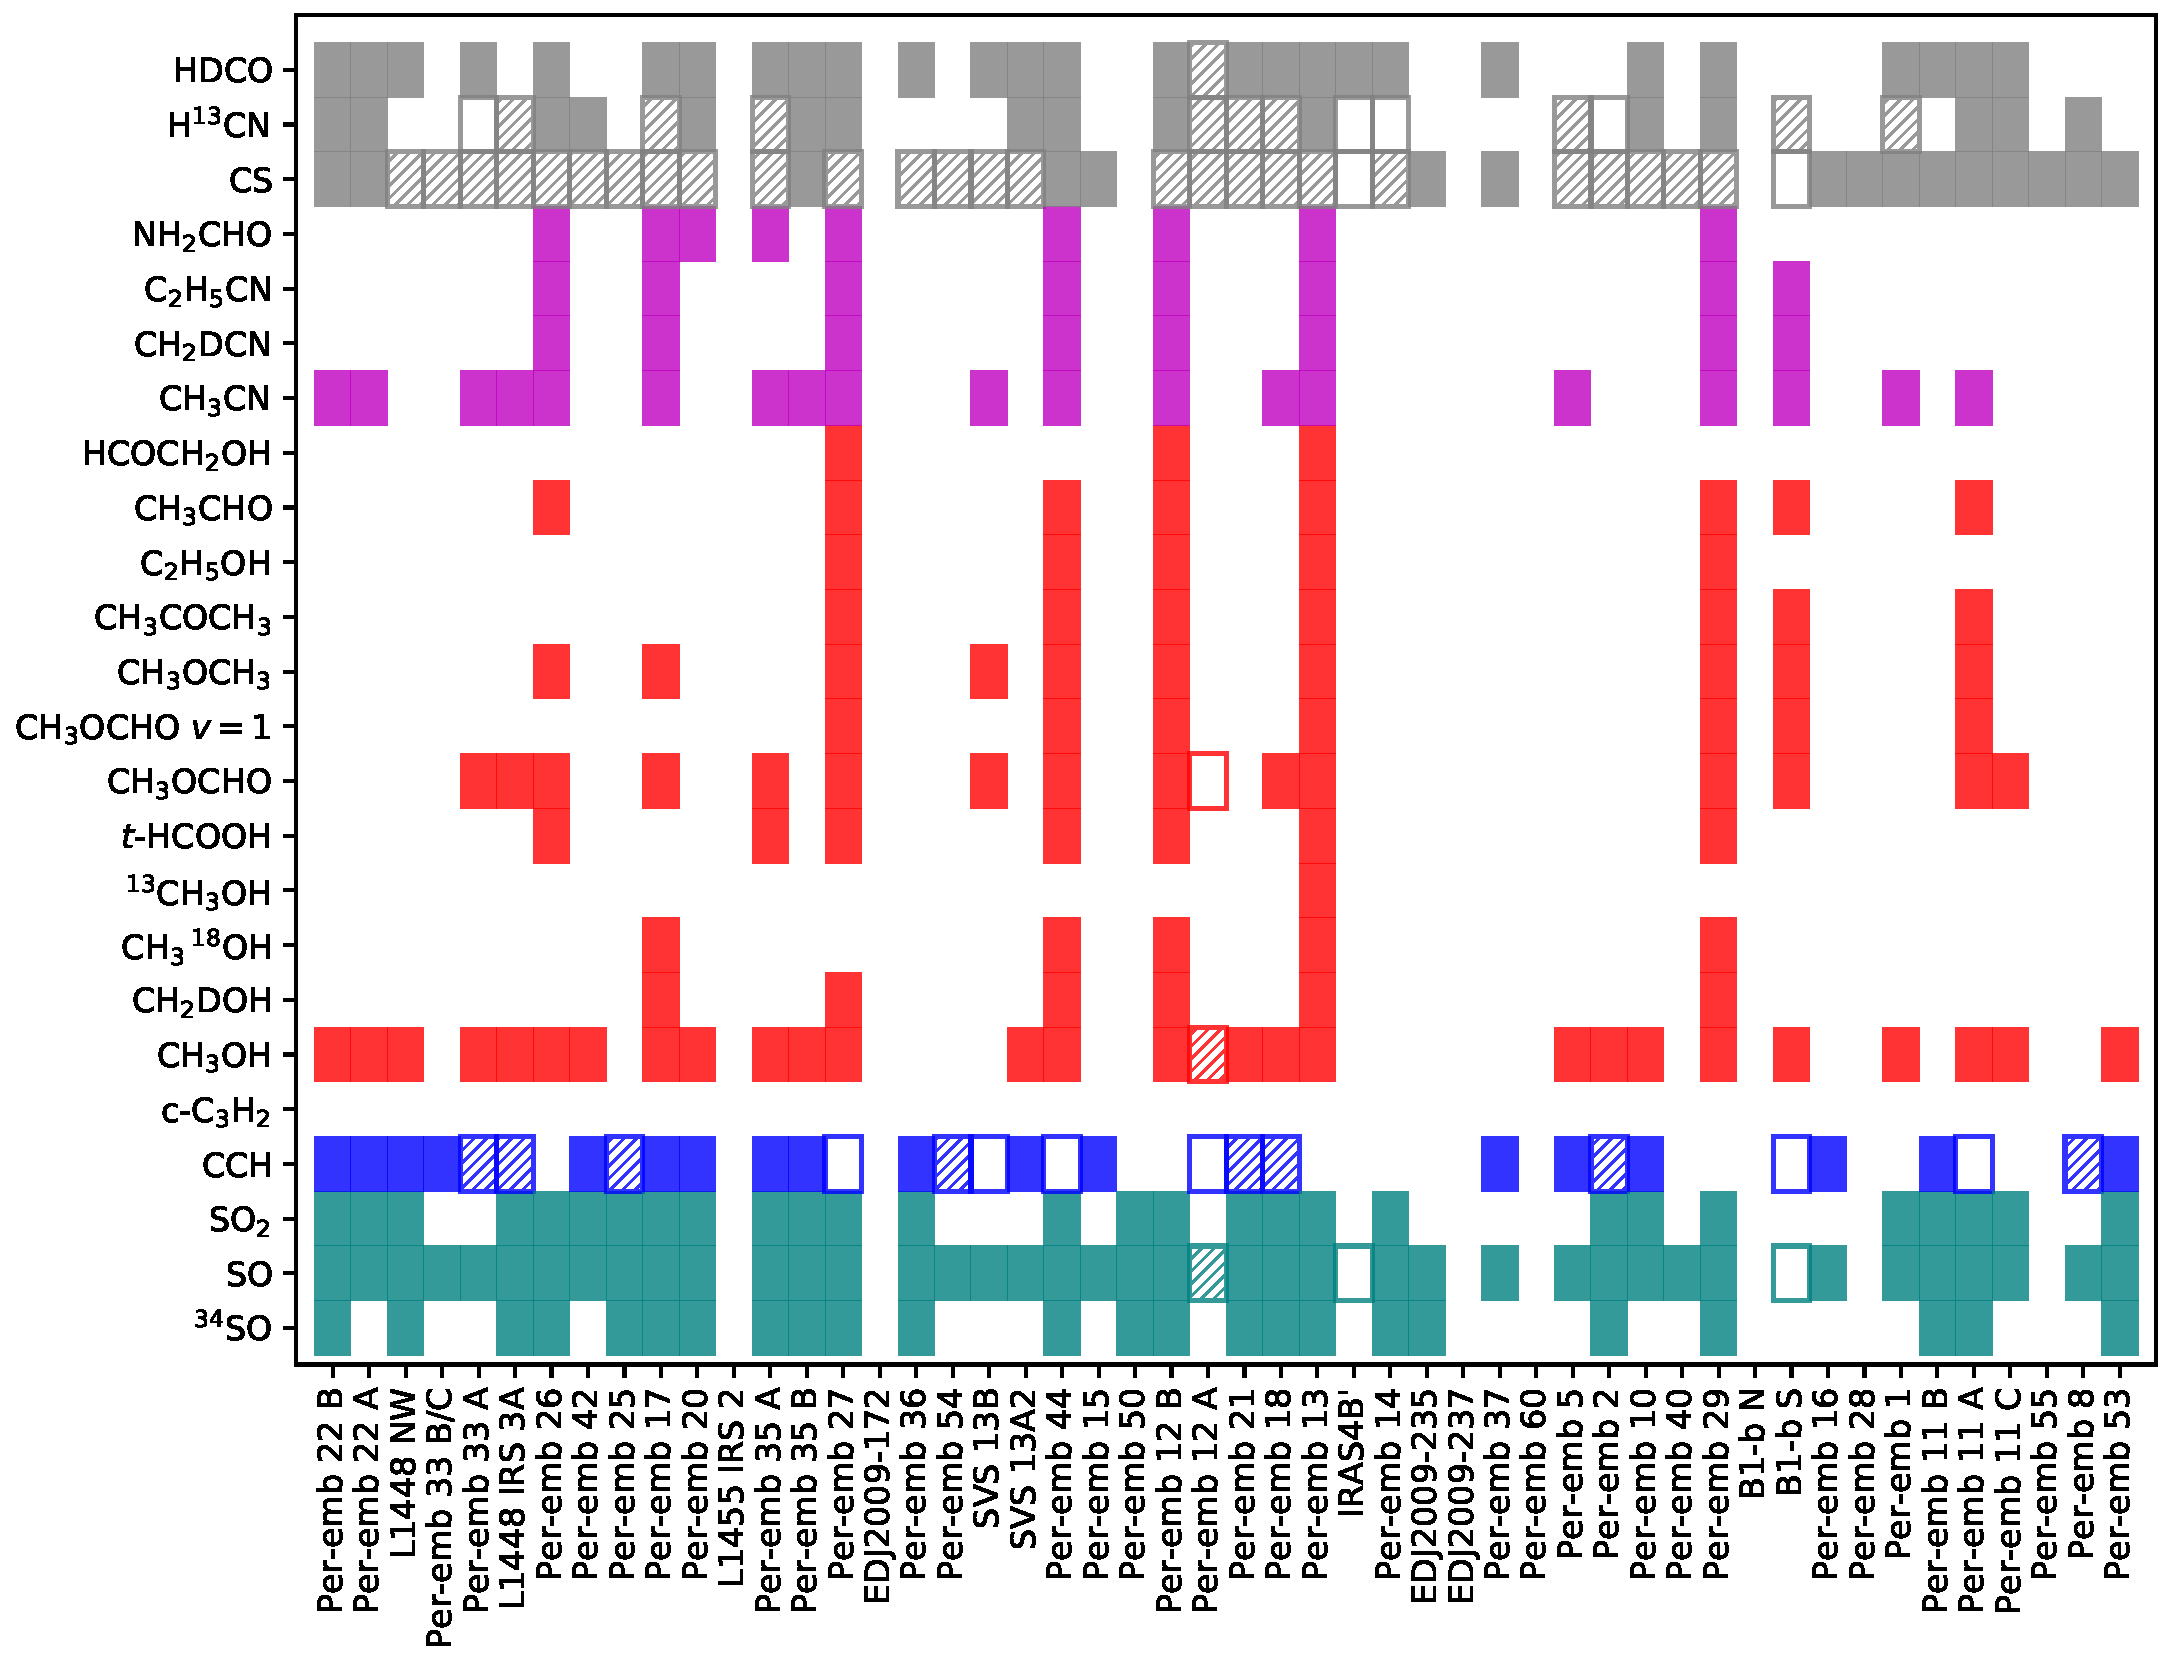
\includegraphics[width=\textwidth]{stats.pdf}
  \caption{Summary of molecular detections.  The sources are sorted by increasing R.A. from left to right.  The detections are color-coded by the types of species: S-bearing molecules in green, carbon-chain molecules in blue, O-bearing COMs in red excluding N-bearing molecules, N-bearing COMs in magenta, other simple organics in gray.  The boxes with solid colors indicate emission and the empty boxes indicate absorption.  The hatched boxes indicate both emission and absorption are seen.}
  \label{fig:stats}
\end{figure*}

\begin{figure*}[htbp!]
  \centering
  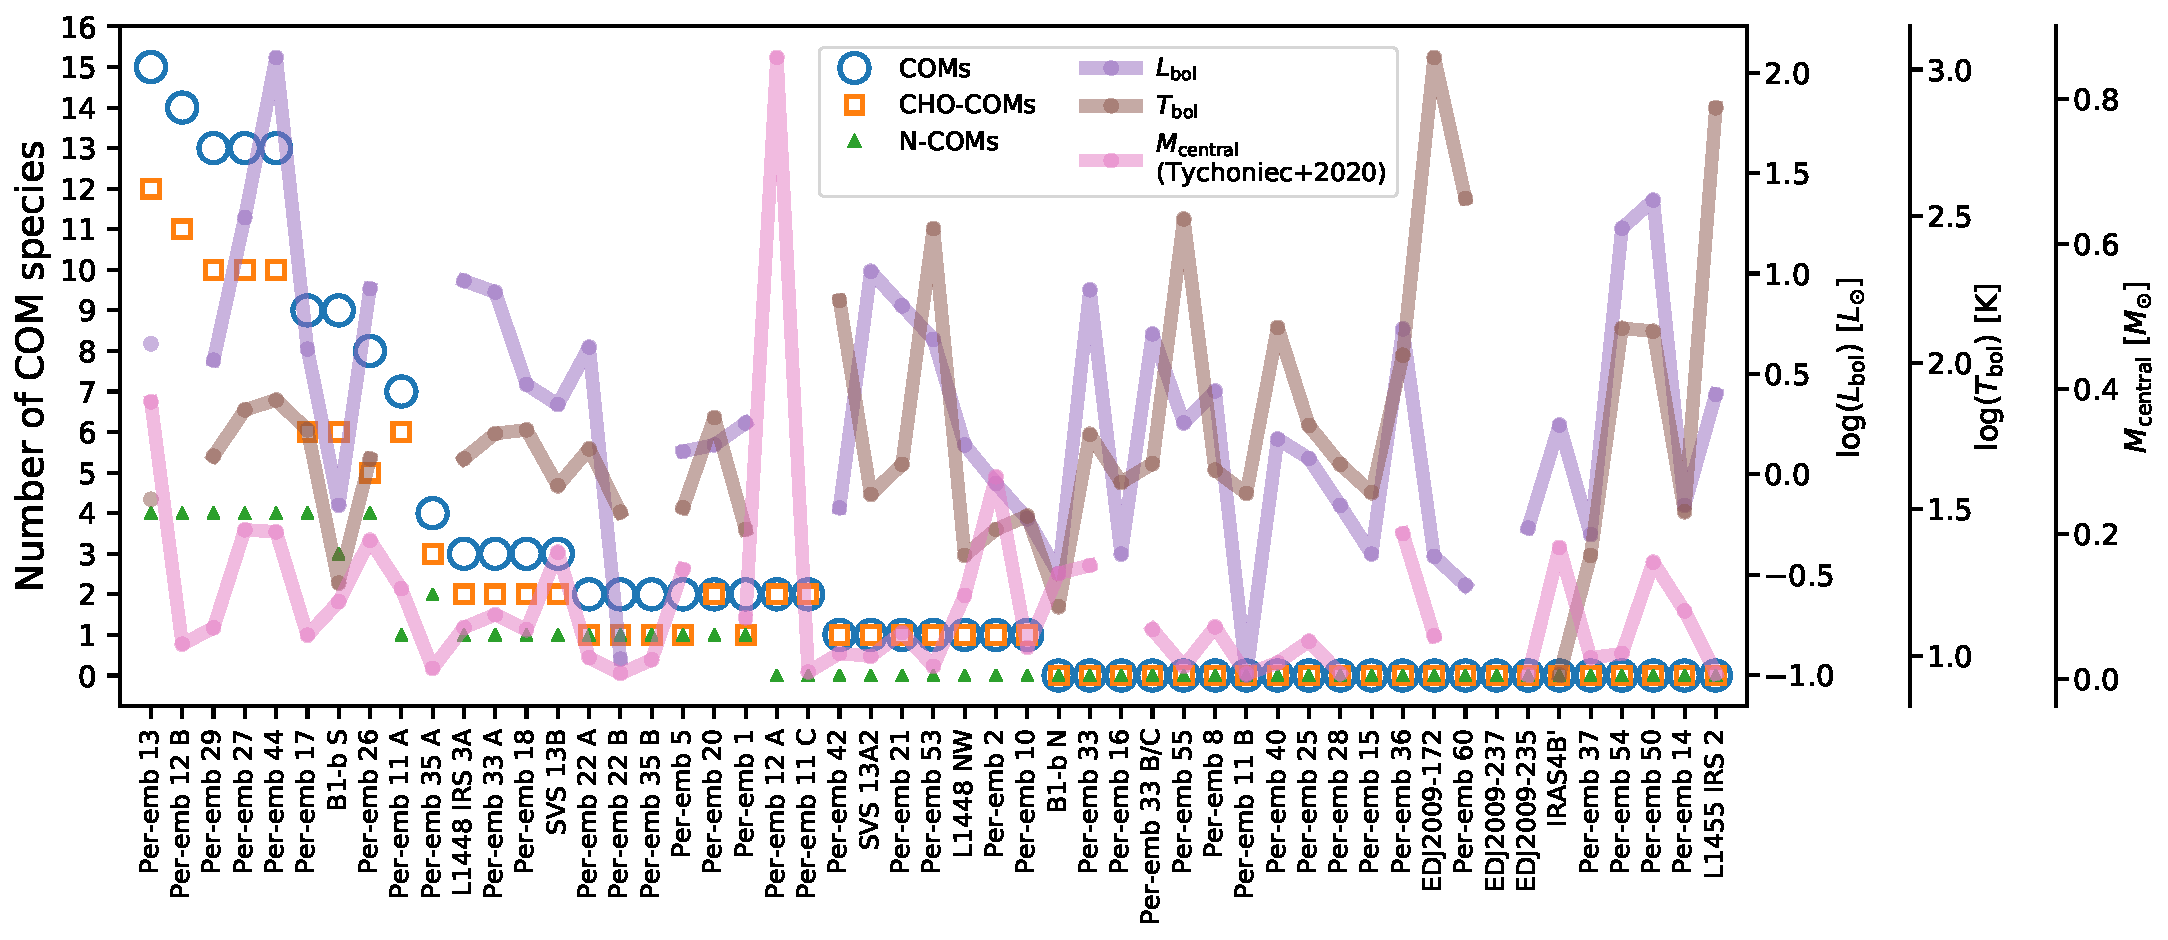
\includegraphics[width=\textwidth]{detection_summary_all.pdf}
  \caption{The number of COMs detected toward the PEACHES sources compared with the bolometric luminosity (purple), the bolometric temperature (brown), and the central dust mass (pink, \citet{2020arXiv200602812T}).  The sources are sorted by the total number of COMs with the number of O-bearing COMs, N-bearing COMs, and all COMs labeled as orange boxes, green triangles, and blue circles, respectively.  The mass of unresolved systems is estimated as the sum of each protostar.  The bolometric luminosities and the bolometric temperatures are taken from \citet{2016ApJ...818...73T} and \citet{2016A&A...592A..56M}.}
  \label{fig:detection_summary}
\end{figure*}

\begin{figure*}[htbp!]
  \centering
  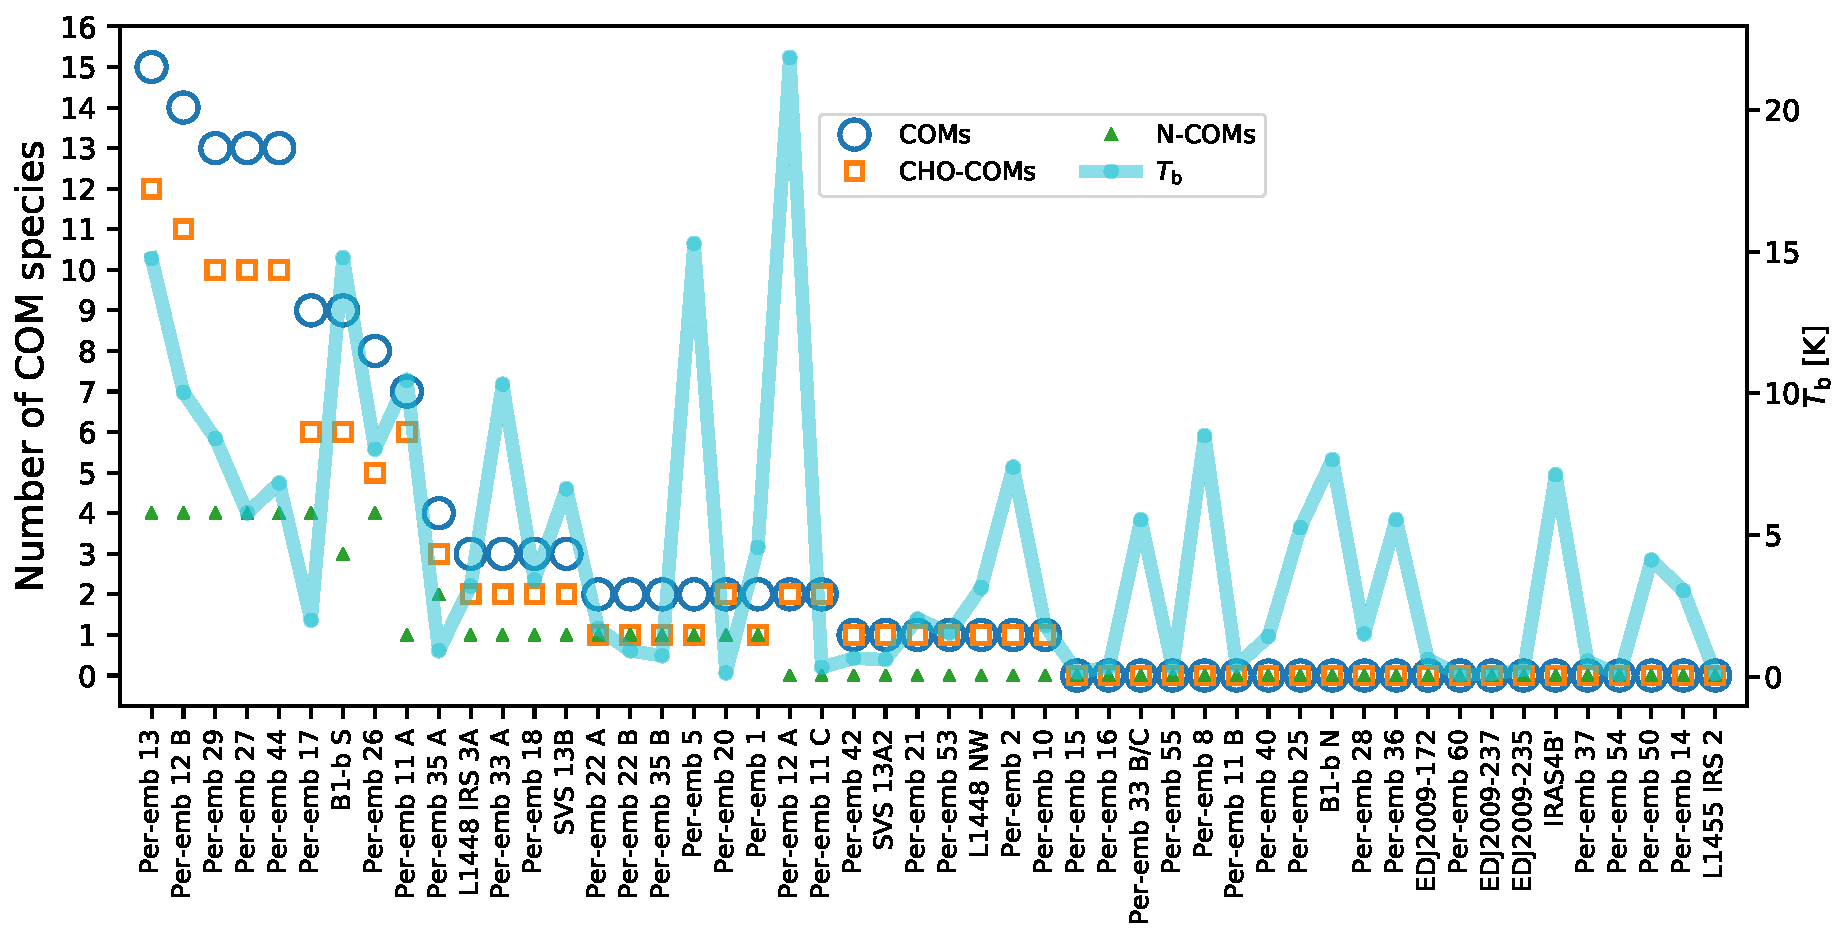
\includegraphics[width=\textwidth]{detection_summary_Tb.pdf}
  \caption{The number of COMs detected toward the PEACHES sources compared with the continuum brightness temperature.  The legends for the protostars are the same as Figure\,\ref{fig:detection_summary}.  The brightness temperatures are indicated in green.}
  \label{fig:detection_summary_Tb}
\end{figure*}

\subsection{Column Densities}
\subsubsection{Excitation Temperatures}
The PEACHES spectra cover four methanol lines, while the spectra of each source include three of them due to the frequency shift in the wide spectral window.  The three methanol lines have upper energy ranging from $\sim$50\,K to $\sim$500\,K, which allows us to estimate the rotational temperature of methanol if all three lines are detected.  To construct the methanol rotational diagram, we fit the methanol emission with a Gaussian profile and bootstrap the measurements for fitting the rotational temperature.  Figure\,\ref{fig:rot_dia_example} shows the rotational diagram of Per-emb 22 B along with the sampled rotational temperature.  The derived rotational temperature of methanol ranges from 120\,K to 240\,K with an exception of Per-emb 18, which has a rotational temperature of 395.7\,K for methanol (Table\,\ref{tbl:methanol_rot_temps}).

\begin{figure*}[htbp!]
  \centering
  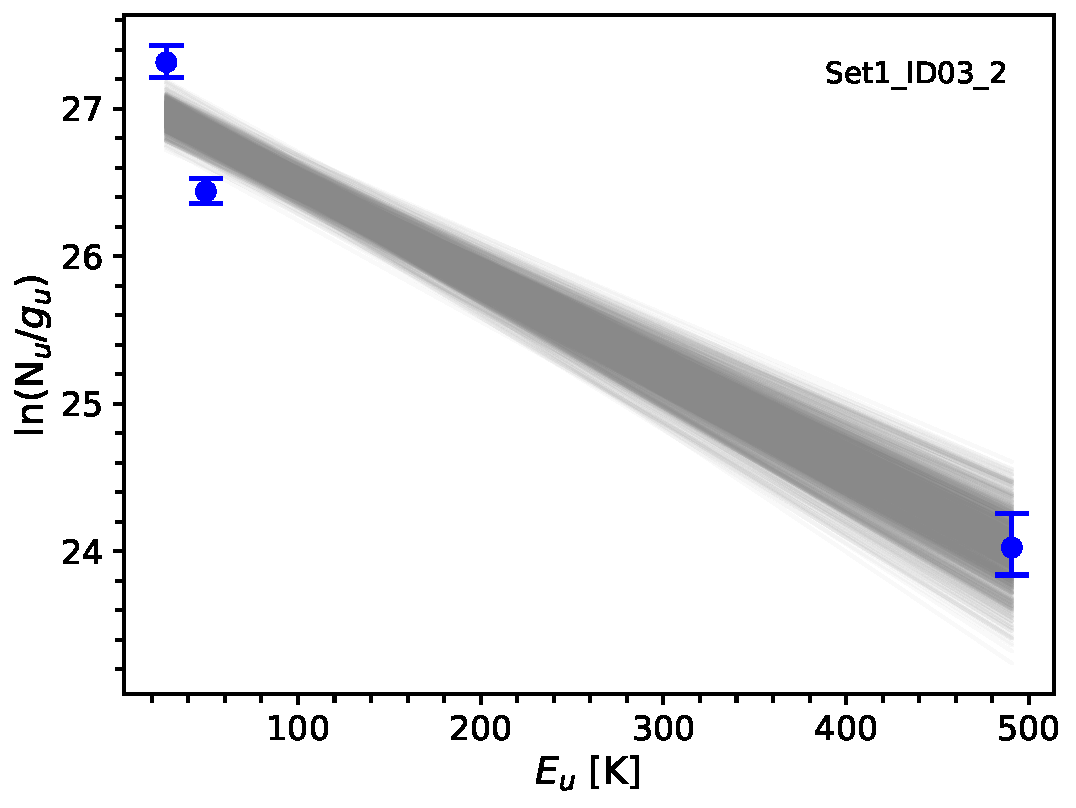
\includegraphics[width=0.47\textwidth]{Set1_ID03_2.pdf}
  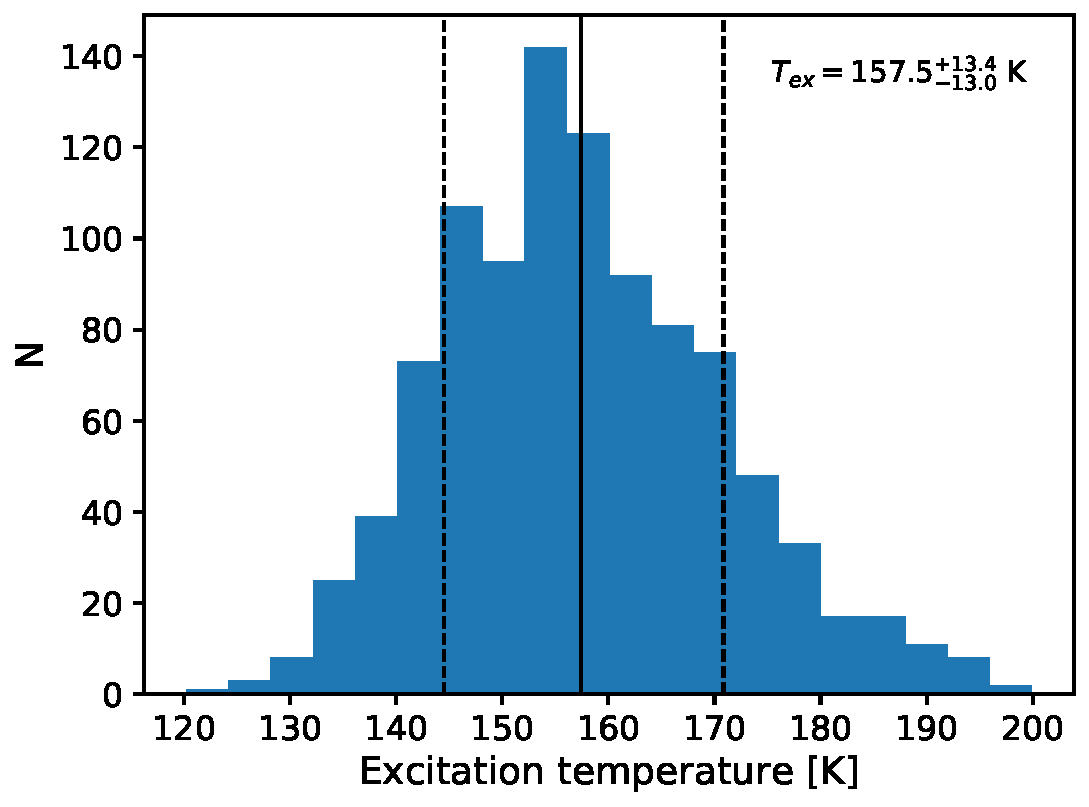
\includegraphics[width=0.47\textwidth]{Set1_ID03_2_rot_temps.pdf}
  \caption{The methanol rotational diagram for Per-emb 22B and the fitted excitation temperature distribution using the bootstraping method.}
  \label{fig:rot_dia_example}
\end{figure*}

\begin{deluxetable}{cc}
  \tabletypesize{\scriptsize}
  \tablecaption{Rotational Temperatures of Methanol \label{tbl:methanol_rot_temps}}
  \tablewidth{0.45\textwidth}
  \tablehead{\colhead{Source} & \colhead{$T_\text{rot}$}}
  \startdata
  Per-emb 26   & 120.1\unc{2.6}{2.5} K   \\
  Per-emb 22 A & 182.4\unc{11.2}{11.4} K \\
  Per-emb 22 B & 157.5\unc{13.4}{13.0} K \\
  Per-emb 17   & 173.9\unc{1.8}{1.9} K   \\
  Per-emb 44   & 197.5\unc{0.3}{0.3} K   \\
  Per-emb 12 B & 194.0\unc{0.8}{0.8} K   \\
  Per-emb 13   & 208.6\unc{3.9}{4.0} K   \\
  Per-emb 27   & 195.8\unc{0.4}{0.4} K   \\
  Per-emb 21   & 151.0\unc{14.6}{15.6} K \\
  Per-emb 35 A & 145.1\unc{3.7}{3.7} K   \\
  Per-emb 18   & 395.7\unc{30.7}{30.4} K \\
  B1-bS        & 241.7\unc{11.7}{11.9} K \\
  Per-emb 29   & 227.7\unc{3.2}{3.3} K   \\
  \enddata
\end{deluxetable}

\textcolor{red}{YLY: need to redo the MCMC fitting.  The fitting shown here is $\sim$6 months old.}  For the sources with significant emission of \methylformate, the column density and the excitation temperature of \methylformate\ can be constrained with MCMC.  Table\,\ref{tbl:mf_temp} lists the sources where the MCMC fitting is feasible and the derived properties of \methylformate.  The best-fitting temperatures range from 100-300\,K with a few outliers at $\sim$1000\,K.  The spectra with the high excitation temperature show non-Gaussian line profiles, making the fitting inaccurate.  Therefore, we exclude those sources in Table\,\ref{tbl:mf_temp}.

\begin{deluxetable*}{ccccccc}
    \tabletypesize{\scriptsize}
    \tablecaption{MCMC Fitting of Methyl Formate \label{tbl:mf_temp}}
    \tablewidth{\textwidth}
    \tablehead{\colhead{Source} & \multicolumn{2}{c}{Temperature [K]} & 
               \multicolumn{2}{c}{log($\mathcal{N}$) [cm$^{-2}$]} & \multicolumn{2}{c}{Line width [km s$^{-1}$]} \\
               \colhead{} & \colhead{best} & \colhead{mode$\pm$HPD} &
               \colhead{best} & \colhead{mode$\pm$HPD} &
               \colhead{best} & \colhead{mode$\pm$HPD}}
    
    \startdata
    Set1\_ID01\_2 & 95 & 76$^{+315}_{-56}$ & 15.24 & 15.29$^{+0.42}_{-0.42}$ & 4.86 & 4.77$^{+0.22}_{-0.52}$ \\
    Set1\_ID02 & 87 & 98$^{+14}_{-41}$ & 15.67 & 15.67$^{+0.10}_{-0.08}$ & 3.66 & 4.06$^{+0.65}_{-0.79}$ \\
    Set1\_ID06 & 93 & 93$^{+59}_{-35}$ & 15.67 & 15.67$^{+0.12}_{-0.08}$ & 4.84 & 4.77$^{+0.22}_{-0.02}$ \\
    Set2\_ID00 & 263 & 310$^{+3}_{-56}$ & 16.89 & 16.92$^{+0.05}_{-0.04}$ & 3.95 & 3.95$^{+0.15}_{-0.12}$ \\
    Set2\_ID01\_2 & 217 & 194$^{+75}_{-4}$ & 16.37 & 16.36$^{+0.10}_{-0.03}$ & 2.22 & 2.25$^{+0.14}_{-0.12}$ \\
    Set2\_ID02 & 195 & 225$^{+119}_{-64}$ & 16.04 & 16.10$^{+0.20}_{-0.09}$ & 1.21 & 1.21$^{+0.00}_{-0.01}$ \\
    Set2\_ID07 & 152 & 131$^{+281}_{-120}$ & 14.79 & 14.72$^{+0.53}_{-0.43}$ & 3.24 & 1.66$^{+2.26}_{-0.40}$ \\
    Set2\_ID08 & 159 & 10$^{+551}_{-0}$ & 14.75 & 14.11$^{+0.85}_{-0.04}$ & 2.37 & 1.20$^{+2.15}_{-0.00}$ \\
    Set2\_ID12 & 115 & 41$^{+269}_{-30}$ & 14.96 & 15.02$^{+0.05}_{-0.94}$ & 4.54 & 4.89$^{+0.09}_{-1.70}$ \\
    Set3\_ID00 & 98 & 58$^{+41}_{-14}$ & 15.85 & 15.82$^{+0.26}_{-0.09}$ & 1.24 & 1.25$^{+0.02}_{-0.05}$ \\
    Set3\_ID01 & 134 & 134$^{+13}_{-27}$ & 16.59 & 16.60$^{+0.02}_{-0.02}$ & 3.04 & 3.08$^{+0.18}_{-0.15}$ \\
    Set3\_ID07 & 104 & 92$^{+182}_{-45}$ & 15.67 & 15.67$^{+0.29}_{-0.15}$ & 2.44 & 2.33$^{+1.22}_{-0.66}$ \\
    \enddata
\end{deluxetable*}


\textcolor{pink}{[put the derived values from HCOOCH3 for several sources. and say consistency with several other works.]
[Put the discussions in 6.1.1. in your section number, and say consistency with HCOOCH3].
[say the assumption/justification of T for sources without multiple line detections(i.e. sources, which is difficult to derive T).  It could partly be overlapped with the section 3.2 (3.1 in your numbering)]}

\subsection{Correlations of COMs}
The chemical evolution of protostars may leave certain patterns in the abundance of molecules as the dynamical evolution determines the density and temperature structures, which regulate chemical reactions.  Thus, the abundance of COMs and their correlations provide critical information to constrain the chemical evolution at embedded protostars.

As described in Section\,\ref{sec:modeling}, we fit the column density and line width with different excitation temperatures, resulting in a range of column density as its uncertainty.  
To quantify the goodness of correlation, we calculate the Pearson's correlation coefficient ($r$), which tests the linearity of two variables.  A simple calculation of the Pearson's correlation coefficient would ignore the uncertainties of the column density.  Thus, we use the bootstrapping method to sample the fitted column densities to calculate Pearson's $r$, by assuming a normal distribution centers on the best-fitted values with the uncertainty as the width of the normal distribution.  If we include the upper limits as normal distributions center on zero, the correlation coefficient becomes significantly lower due to the cluster of samples around zero column density (Figure\,\ref{fig:pearson_distribution}).  With the detection-only sample, the mean Pearson's $r_{d}$ is 0.91, as expected for a tight correlation, with a Gaussian-like distribution skewed toward lower values.  After including the upper limits, the mean Pearson's $r$ decreases to 0.59 with larger uncertainty (the 68\%\ credible interval increases by 160\%).  Thus, the bootstrapped correlation coefficient only considers the detections.

Figure\,\ref{fig:corner} shows the correlations of several COMs selected from their detection rates as well as the ratios between species which is discusedd in Section\,\ref{sec:ratios}.  The column density of \methanol\ best correlates with that of \methylcyanide.  \citet{2020A&A...635A.198B} also found the tight correlation between these two molecules from the CALYPSO survey, which has a selective sample.  The column densities of \dimethylether\ and \methylformate\ also show a tight correlation.  \methanol\ also correlates with more complex species (i.e. so called daughter species, \methylformate\ and \dimethylether) with a lower correlation coefficient than that between \methanol\ and \methylcyanide.  The correlations between \methylcyanide\ and more complex species also show the same behavior.  The decreasing strength of correlation with between the simple COMs and more complex COMs supports the hypothesis that \methanol\ and \methylcyanide\ are first generation species and \methylformate\ and \dimethylether\ are the second generation (\refnote).  The correlations of \methanol, \methylcyanide, \methylformate, and \dimethylether\ with other COMs show positive trends; however, the correlations are driven by a few sources due to the low detection rate of other COMs (Figure\,\ref{fig:major_minor}).

The column densities shown in Figure\,\ref{fig:corner} and \ref{fig:major_minor} are the column densities within a 0\farcs{5} region.  The correlations remain similar for the column densities averaged within the extracted region.  To directly compare the abundance of COMs, we normalize the column densities of COMs by the \tbc, which is a proxy of gas column density.  The normalized column densities of COMs show similar correlations as that of the column densities (Figure\,\ref{fig:corner_combined}).  We further normalize the ``abundance'' of COMs ($N_\text{COM}/T_\text{b}$) with \lbol\ and \tbol\ to test the effect of the protostellar evolutionary stage on the observed complex chemistry (Figure\,\ref{fig:corner_combined}, green and orange).  After the normalization with \lbol\ and \tbol, the correlation coefficients remain similar for most cases.  Normalized with \lbol\ and \tbol, the correlation between \methanol\ and \dimethylether\ decreases significantly, while \methylcyanide\ shows a moderate decrease of correlation with \dimethylether.  However, the correlations between \methylformate\ and \dimethylether\ remain similar with different normalizations.  The column densities correlations of \methanol\ \&\ \dimethylether\ and \methylcyanide\ \&\ \dimethylether\ are also lower than that of other combinations of species.  
\textcolor{red}{Thus, the evolutionary stage of protostars plays an insignificant role on determining the abundance of most COMs but has a substantial effect for \dimethylether.}

% The comparison between \cch\ and \methanol\ shows no correlation between these two molecules (Figure\,\ref{fig:cch_ch3oh}), similar to the conclusion in \citet{2018ApJS..236...52H}.  The single dish survey by \citet{2016ApJ...833..125G} shows a correlation between C$_{4}$H, a more complex carbon-chain molecules, and \methanol.  Outflow activity can promote the formation of \cch, which is more efficiency at warm temperature \citep[e.g., ][]{2018ApJ...864...76Z,2019ApJ...873L..21I}.  In face, the morphology of \cch\ often traces the outflow cavities seen from CS.  Therefore, the lack of correlation between \cch\ and \methanol\ may be affected by the inner cavity wall of outflows, because our spectra are taken toward the continuum peak.  Observations with a larger $\theta_\text{MRS}$ will minimize the effect of missing flux in interferometry for a faithful comparison of the \cch\ abundance on the inner envelope.

\begin{figure*}[htbp!]
  \centering
  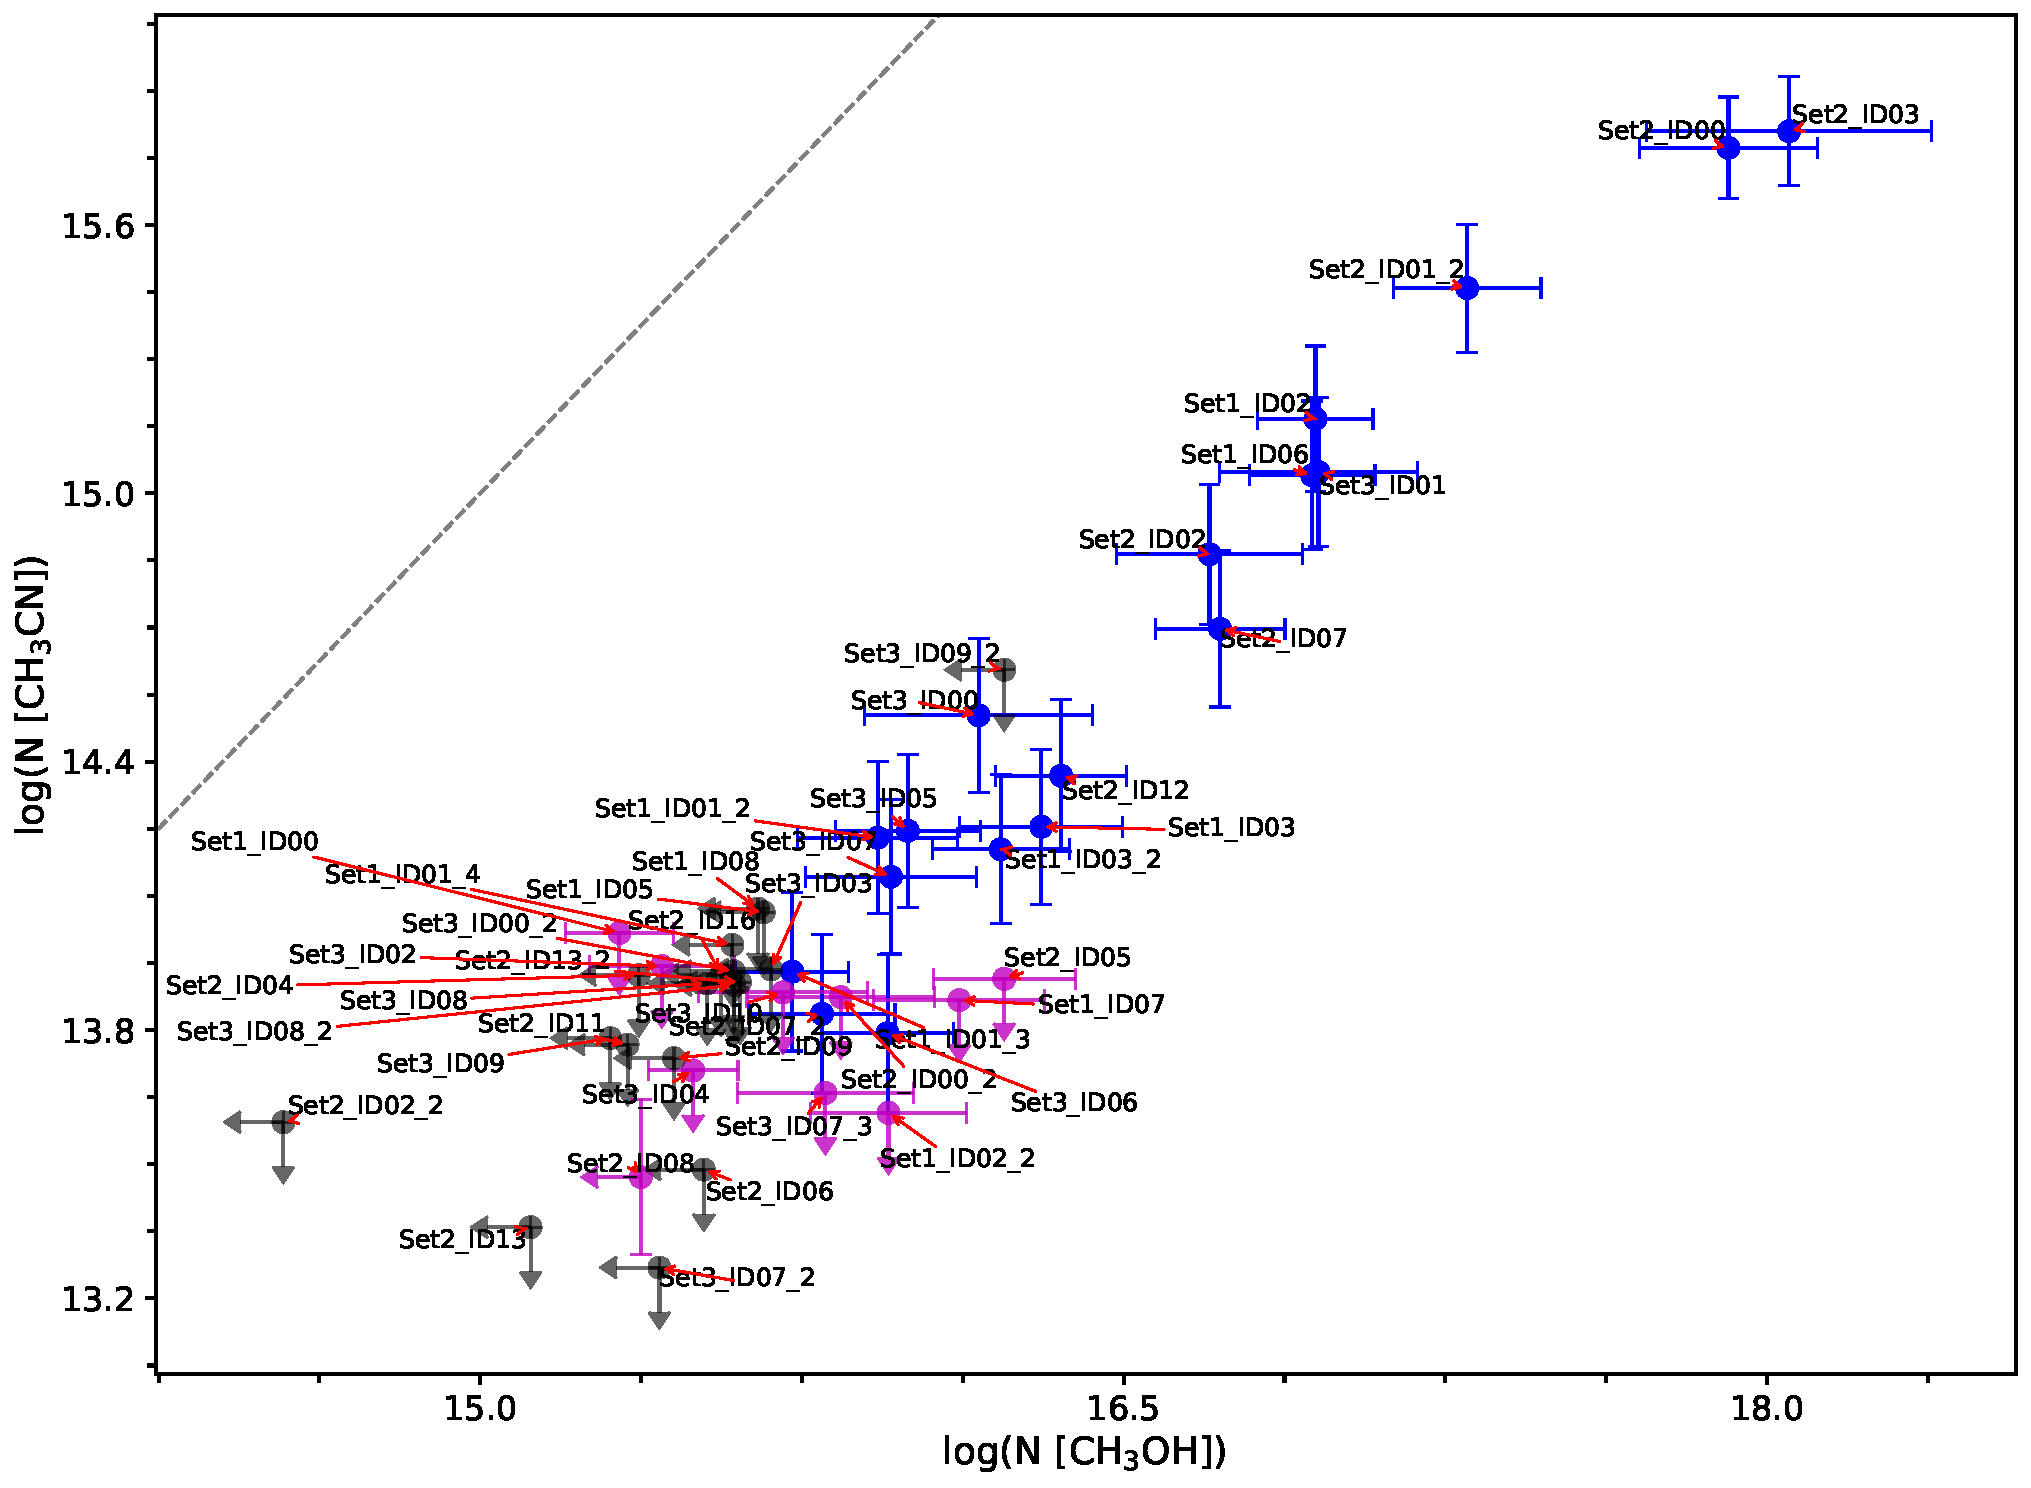
\includegraphics[width=\textwidth]{Ncol_ch3oh_ch3cn.pdf}
  \caption{Correlation of the fitted column densities of \methanol\ and \methylcyanide\ from the PEACHES protostars.  The sources where both molecules are detected are shown in black; the sources where only one molecule is detected are shown in magenta; finally, the sources where both molecules are not detected are shown in black for the corresponding upper limits.}
  \label{fig:ch3oh_ch3cn}
\end{figure*}

\begin{figure}[htbp!]
  \centering
  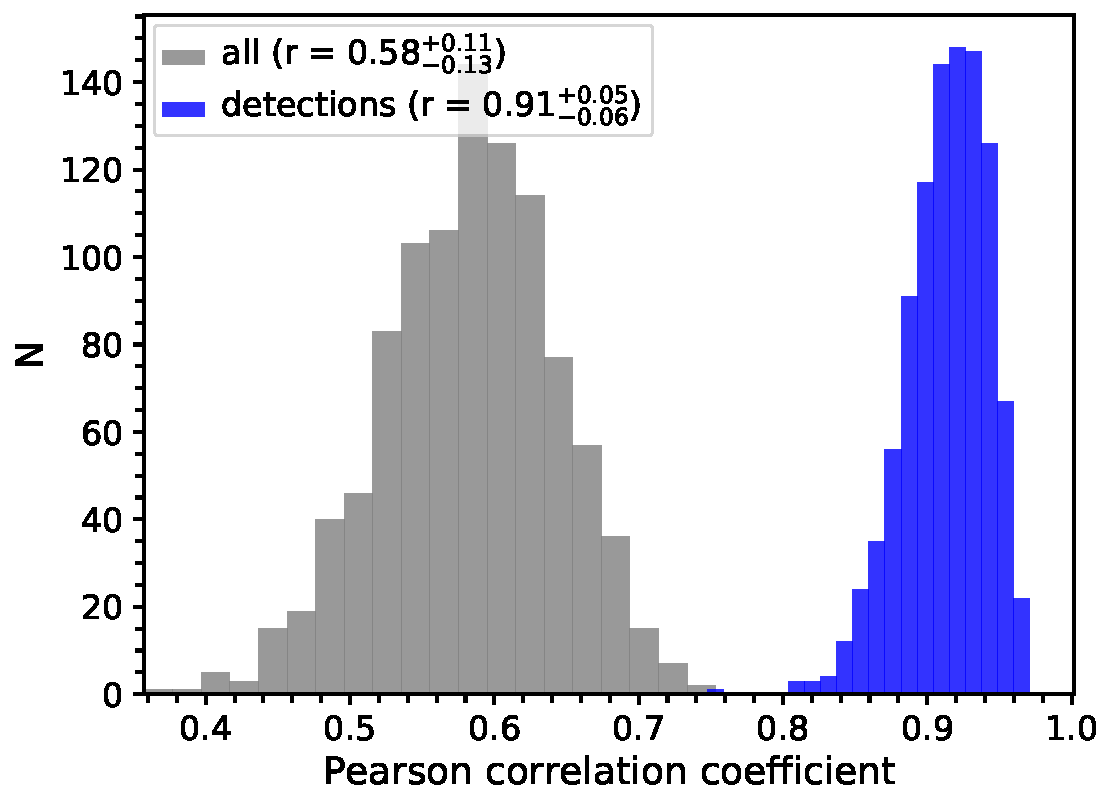
\includegraphics[width=0.47\textwidth]{pearson_r_ch3oh_ch3cn.pdf}
  \caption{Distributions of Pearson's correlation coefficient from 10000 resamples drawn from detections $+$ non-detections and only detections.  The legend indicates the mean values of Pearson's $r$ along with the range of the 95\%\ credible interval as the associated uncertainties.}
  \label{fig:pearson_distribution}
\end{figure}

\begin{figure*}[htbp!]
  \centering
  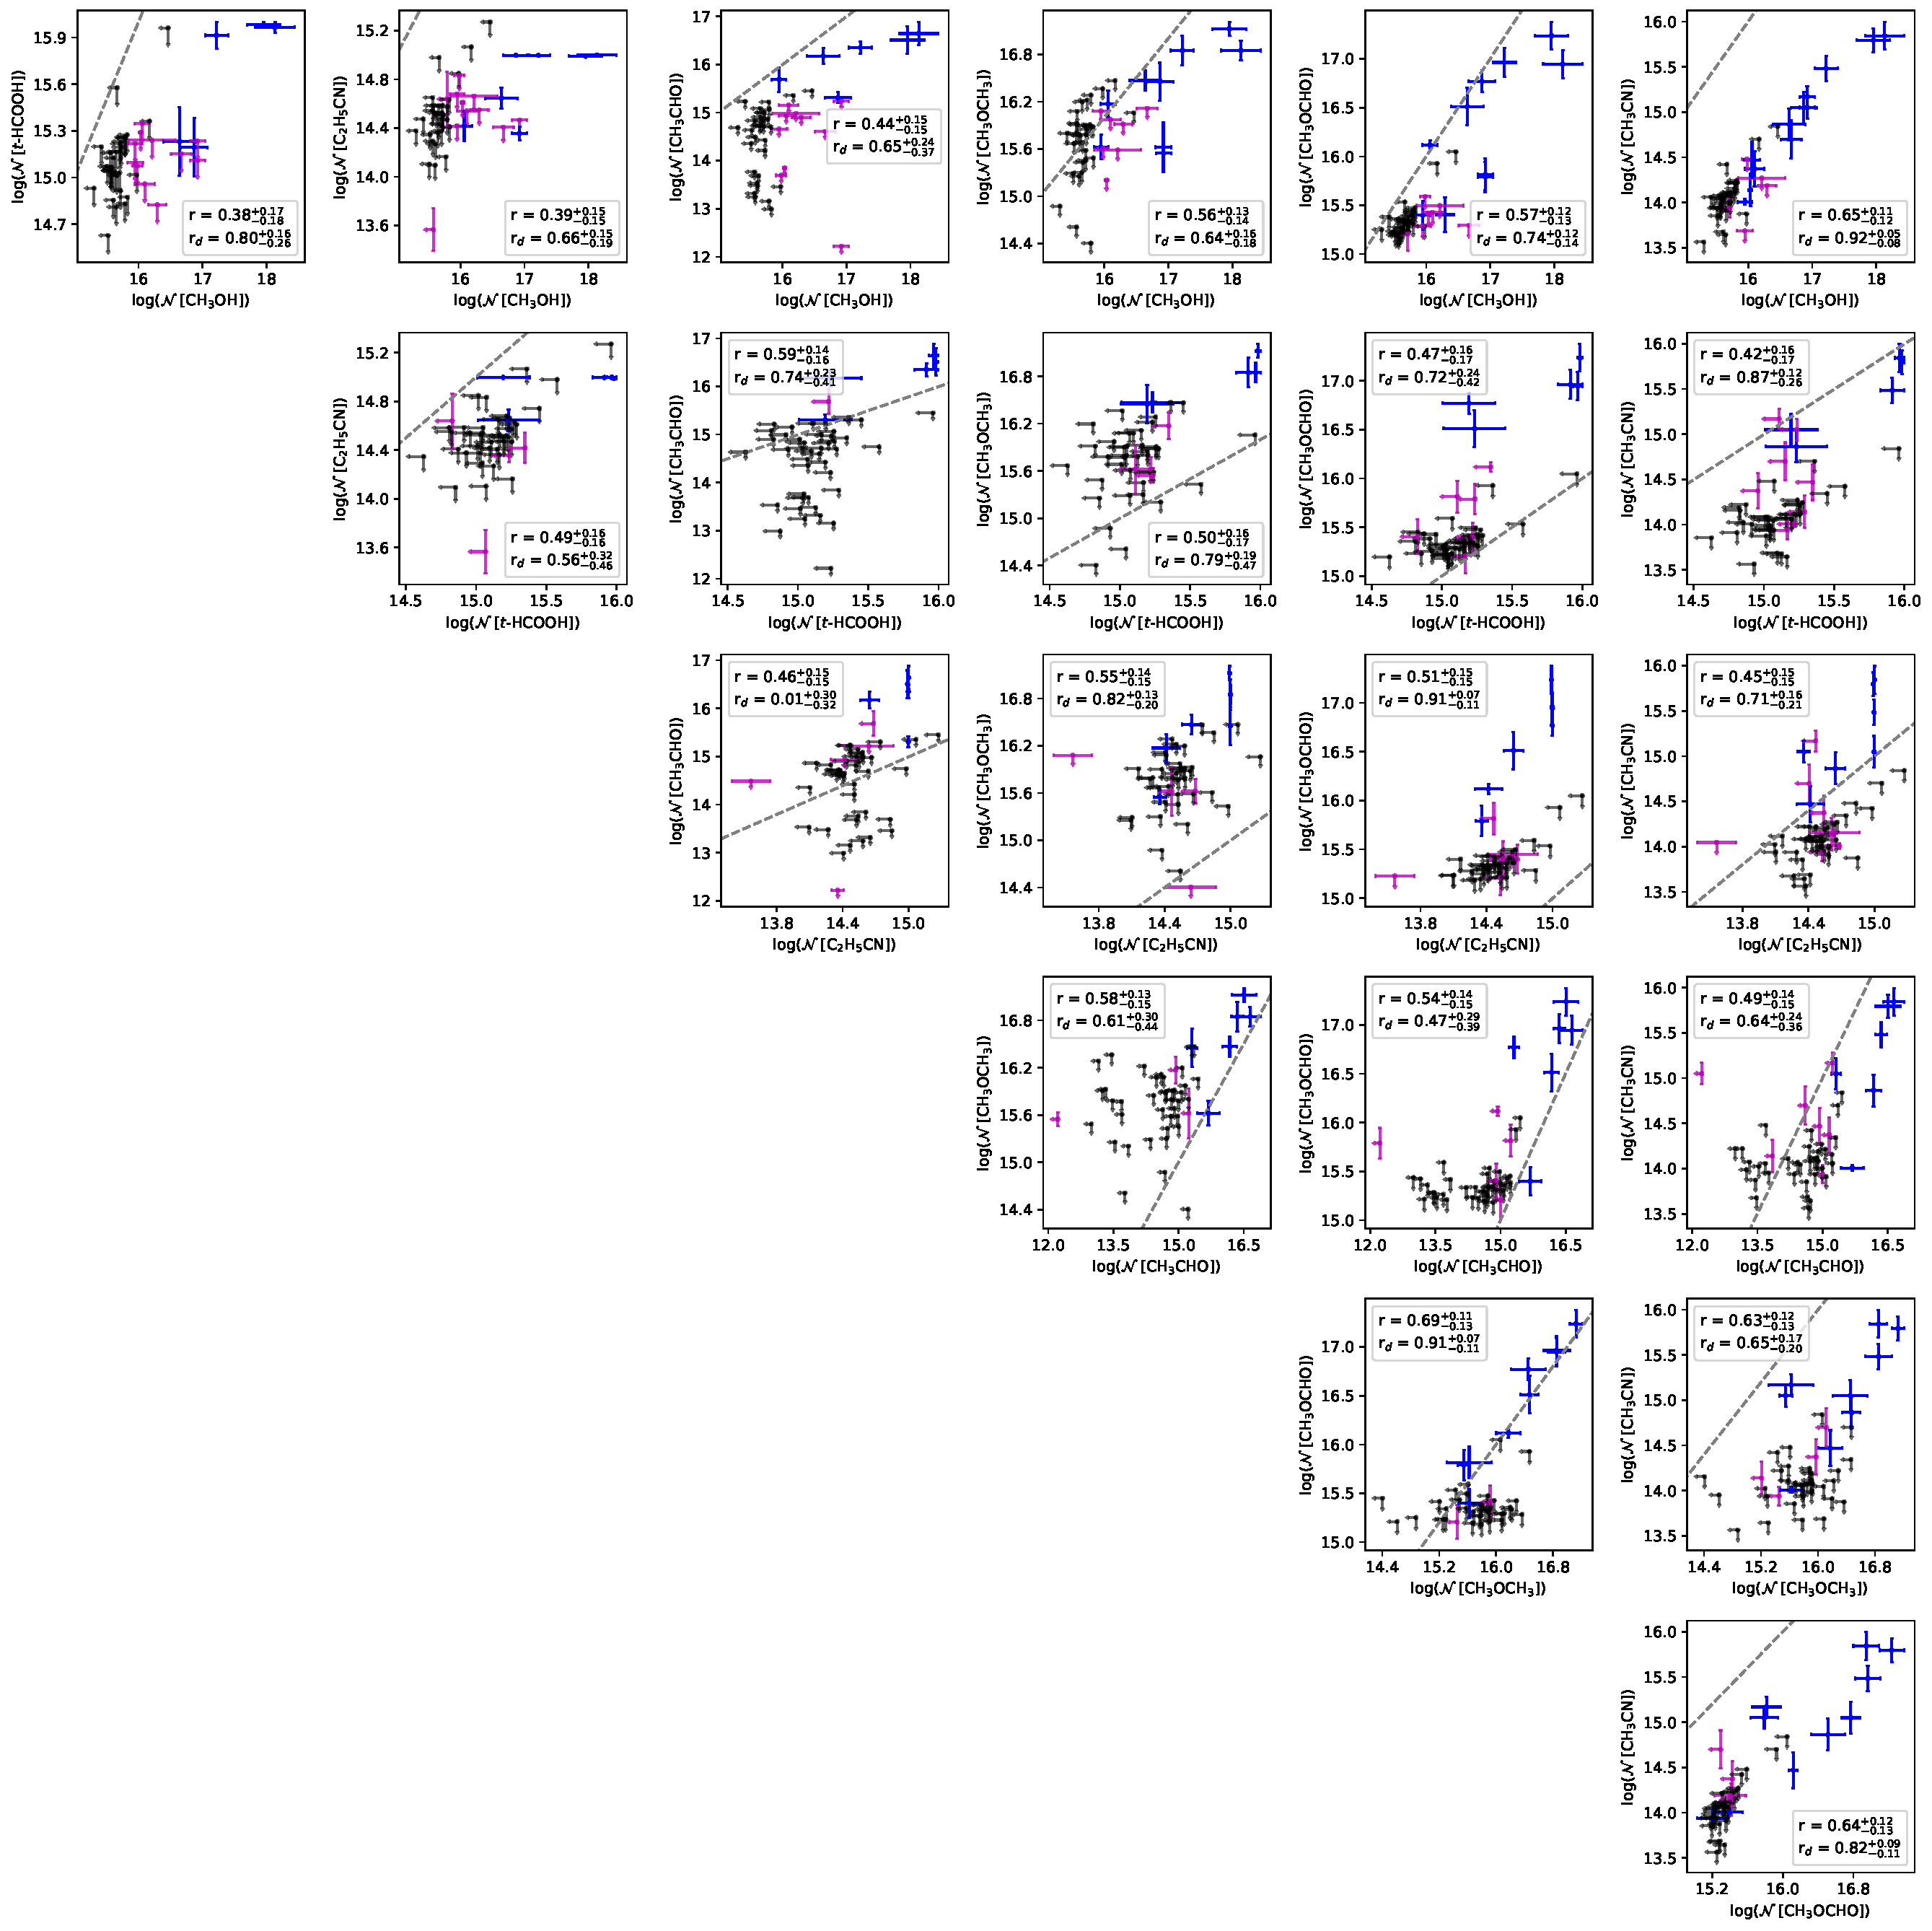
\includegraphics[width=\textwidth]{corner_Ncol_correlations.pdf}
  \caption{Corner plot of the correlations of the column densities between \methanol, \methylcyanide, \methylformate, and \dimethylether.  The color code follows that in Figure\,\ref{fig:ch3oh_ch3cn}.  The dashed line indicates equality.  The legends indicate the Pearson's $r$ for the detection-only sample ($r_{d}$) and the logarithmic ratio of the two molecules (N$_{y}$/N$_{x}$).  The four most detected COMs are shown in this figure, while other COMs are shown in Figure\,\ref{fig:major_minor}.}
  \label{fig:corner}
\end{figure*}

\begin{figure*}[htbp!]
  \centering
  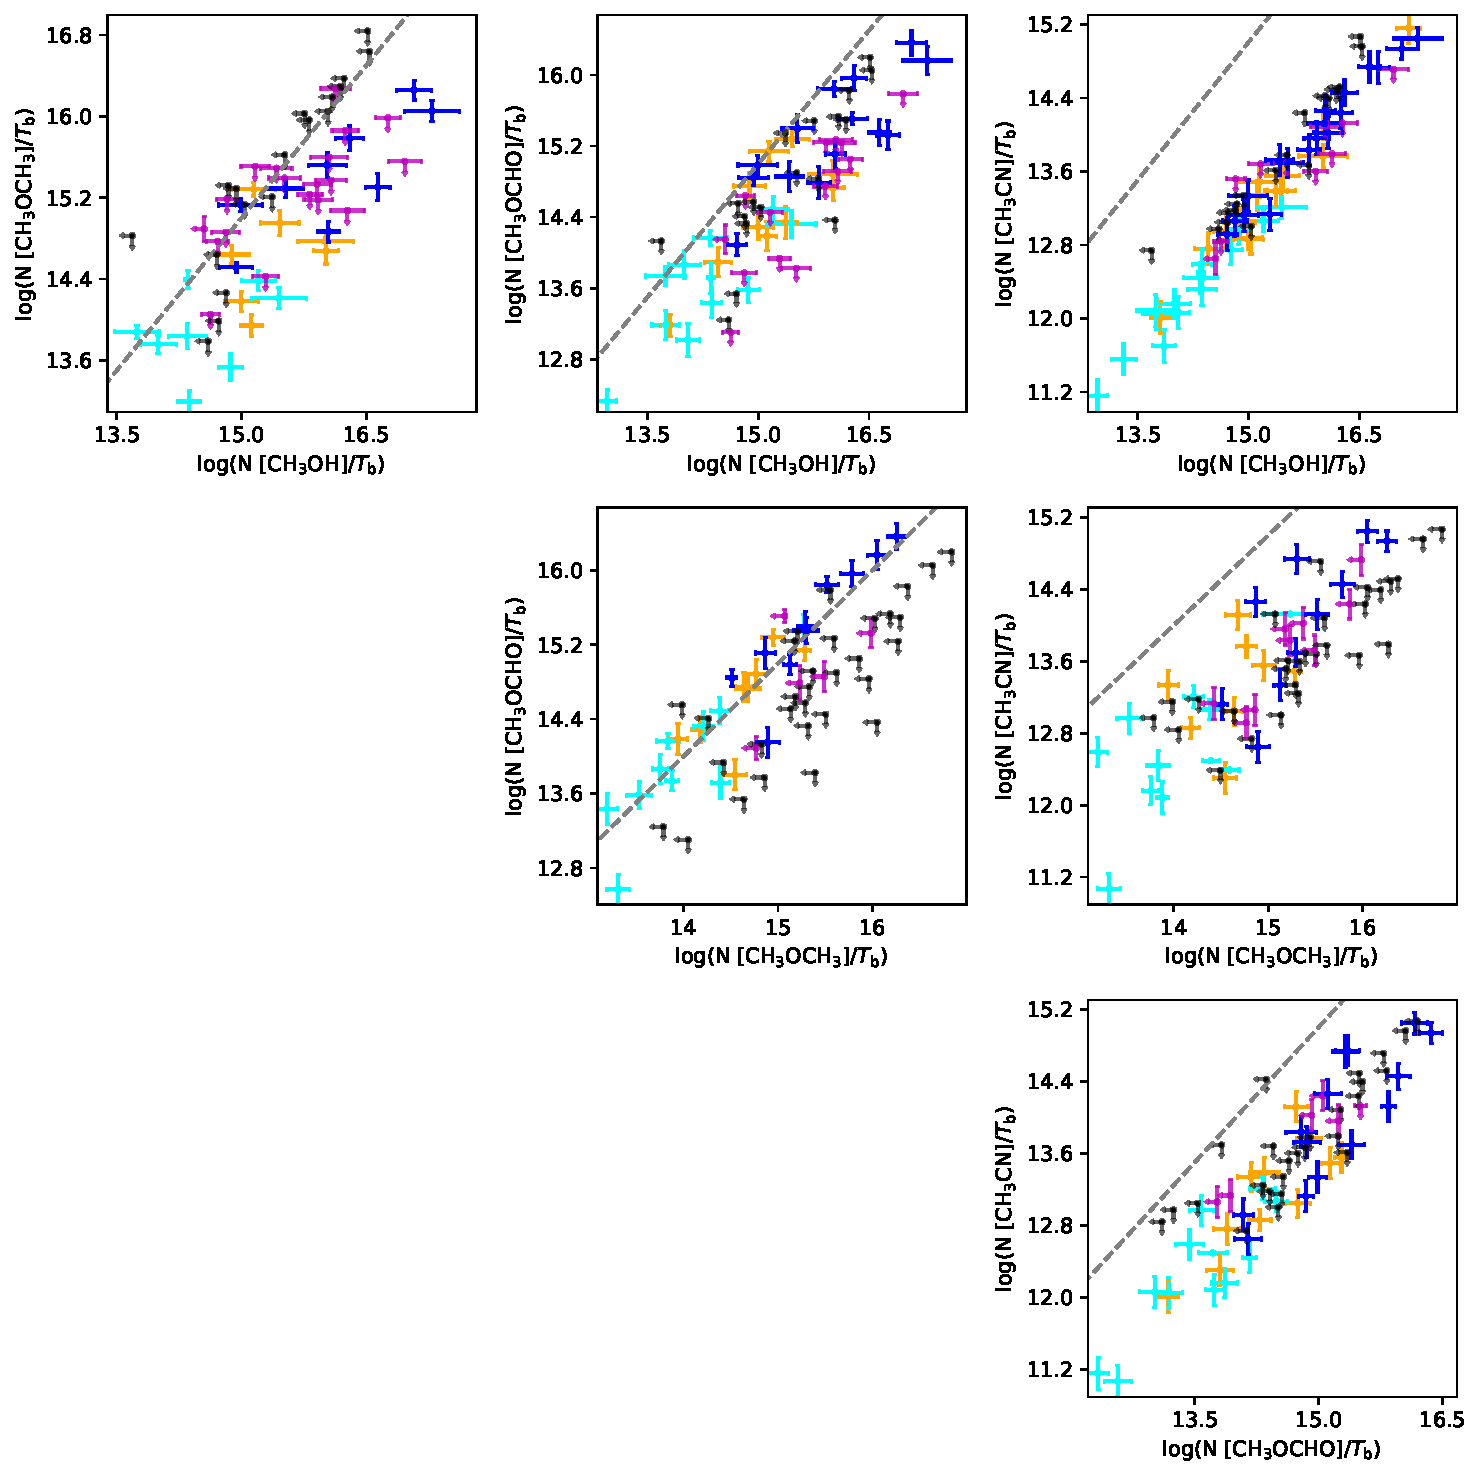
\includegraphics[width=\textwidth]{corner_Ncol_correlations_combined_norm.pdf}
  \caption{Corner plot of the correlations of the normalized column densities.  The blue, magenta, and black symbols indicate the column densities normalized by the continuum brightness temperature (\tbc), while the color scheme follows that in Figure\,\ref{fig:ch3oh_ch3cn}.  The orange symbols show the column densities normalized by \tbc\ and the bolometric luminosity (\lbol), while the green symbols show that normalized by \tbc\ and the bolometric temperature (\tbol).  We only show the column densities if both molecules are detected for the ones normalized by \tbc\tbol\ and \tbc\lbol.  The Pearson's $r$ correlation coefficient for the detections with each normalization is shown in the legend with corresponding color.  A few close multiple sources, including Per-emb 12 A \&\ B, Per-emb 35 A \&\ B, and Per-emb 11 A \&\ C, are excluded for the normalization of \tbol\ and \lbol\ due to their poorly determined SEDs.}
  \label{fig:corner_combined}
\end{figure*}

\begin{figure*}[htbp!]
  \centering
  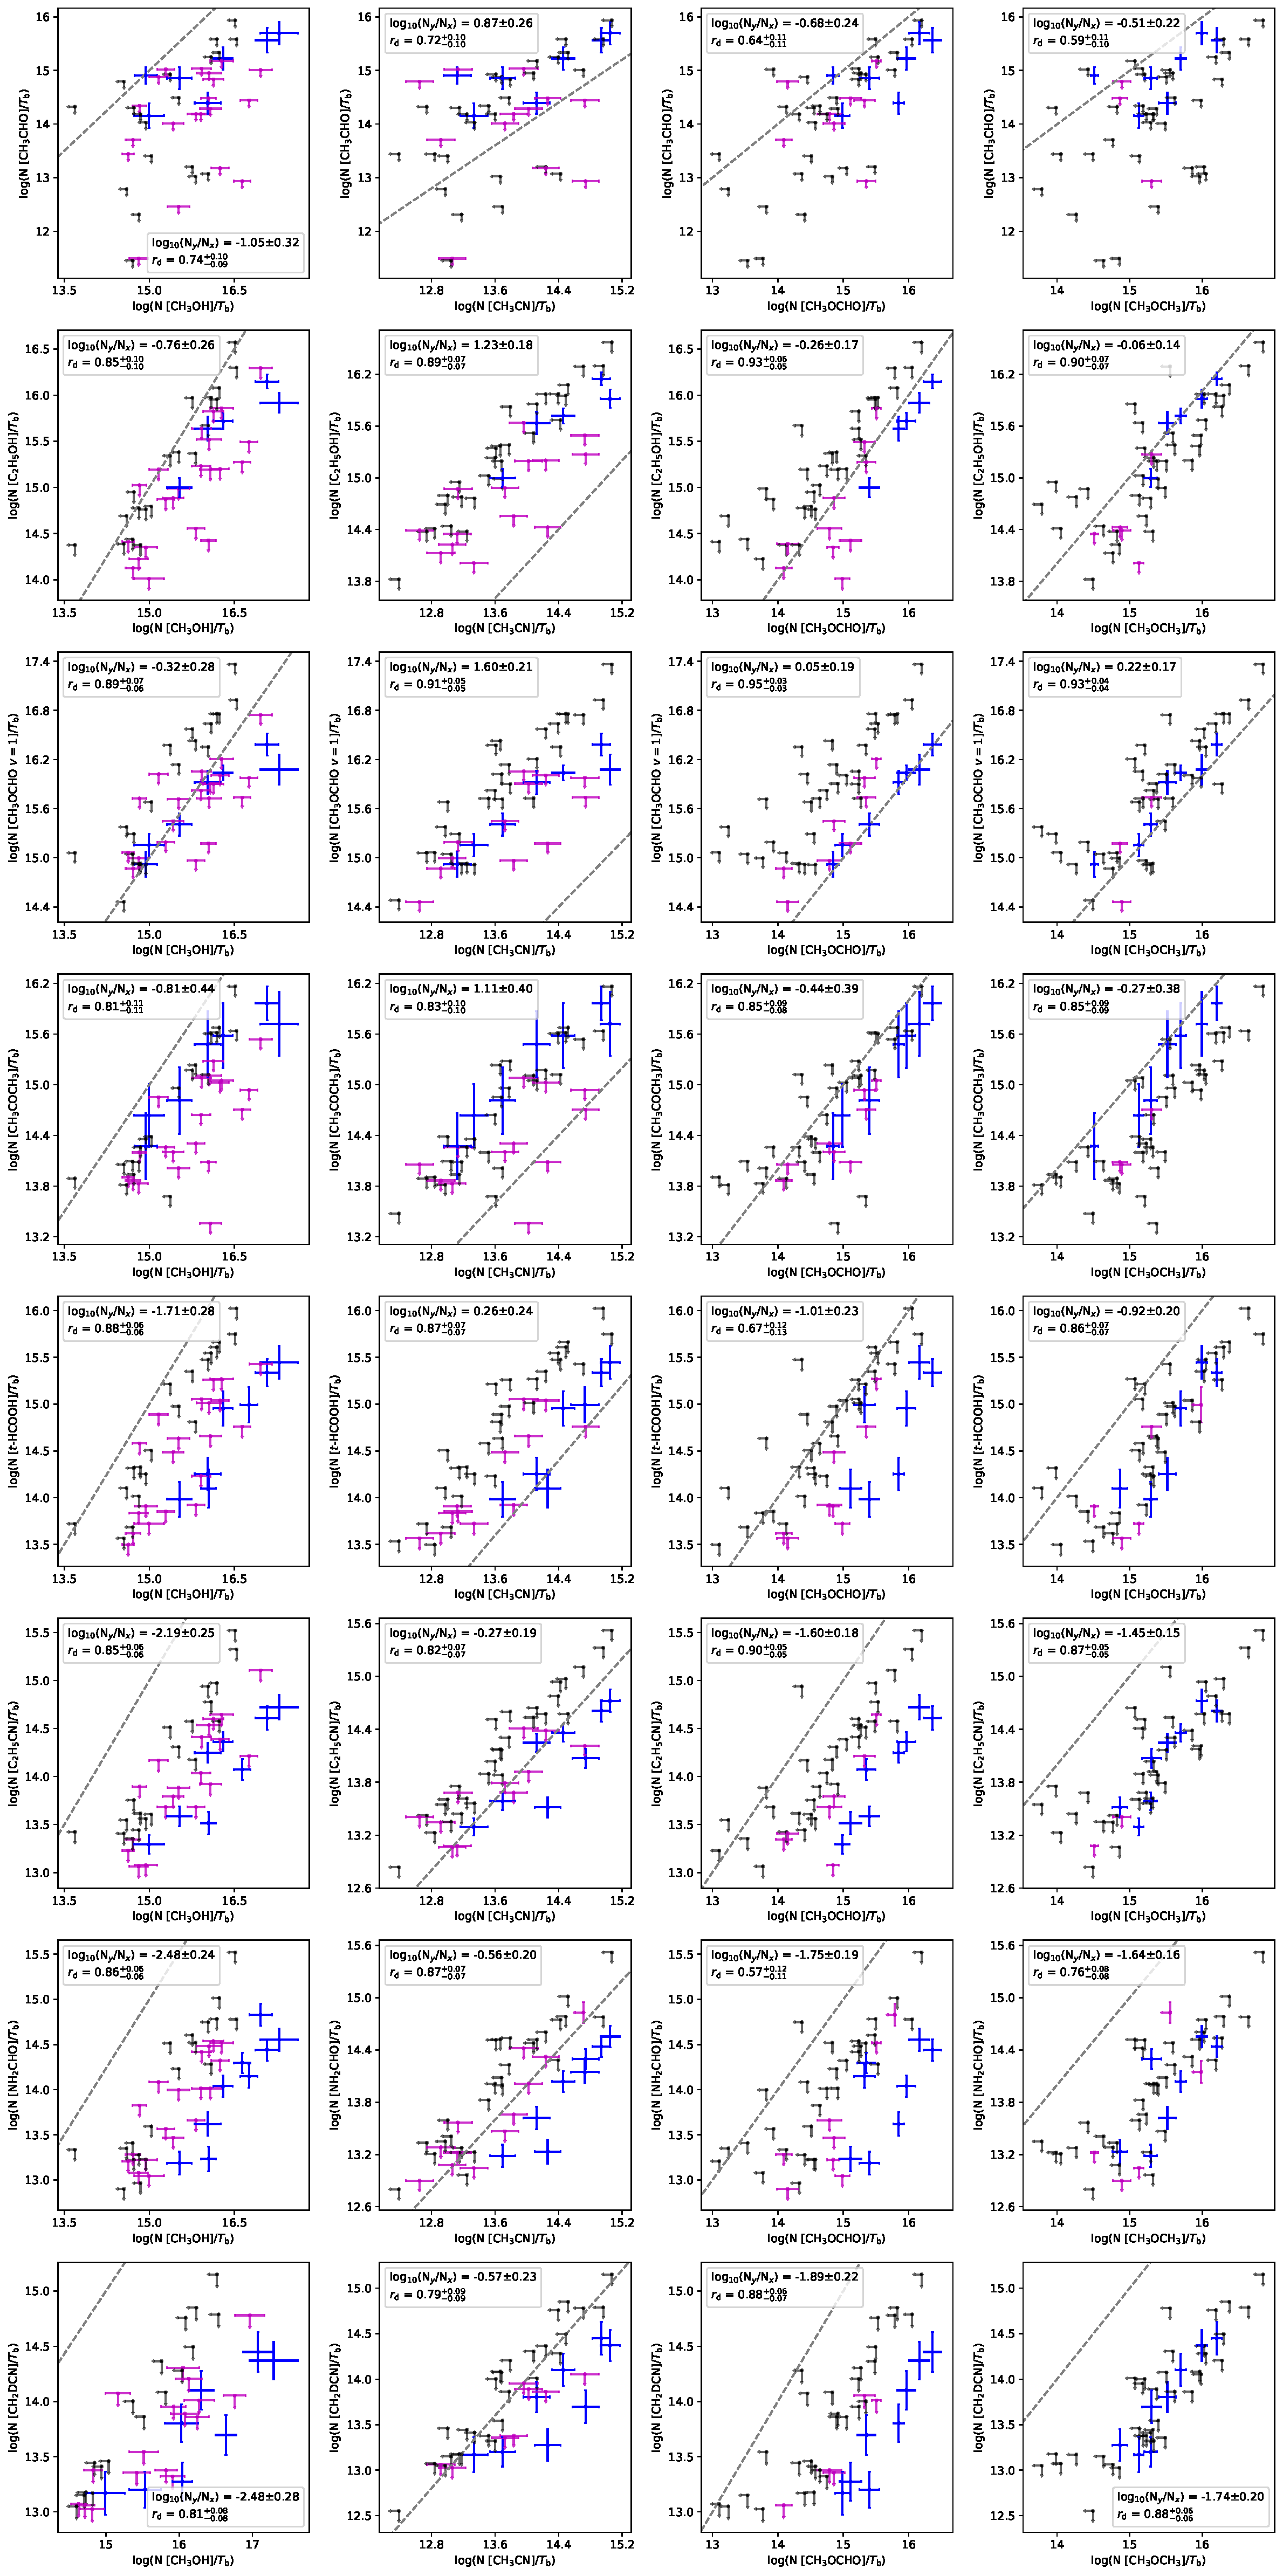
\includegraphics[height=9in]{Ncol_major_minor.pdf}
  \caption{Corner plot of the correlations of the column densities normalized by the continuum brightness temperature between the more abundance COMs, \methanol, \methylcyanide, \methylformate, and \dimethylether, and the less abundance COMs \acetaldehyde, \ethanol, \methylformatev, \acetone, \ethylcyanide, $t$-HCOOH, and \formamide.  The legends are similar to Figure\,\ref{fig:ch3oh_ch3cn}.}
  \label{fig:major_minor}
\end{figure*}

\section{Discussion}
\subsection{Universal Chemistry among Hot Corinos?}
For the protostars with compact emission of COMs, so called hot corinos, the abundance of COMs correlates well between species.  With the normalization of \tbc, the Pearson's $r$ for the correlations between the four major species (\methanol, \methylcyanide, \methylformate, and \dimethylether) are 0.76--0.93 (Figure\,\ref{fig:corner_combined}).  The Pearson's $r$ for the four major species with all COM species has a median value of 0.86 with a range from 0.57 to 0.95 (Figure\,\ref{fig:major_minor}).  The correlations remain strong with the normalizations of \lbol\ and \tbol, suggesting that the chemistry of COMs may be independent of the evolutionary stage of protostars.  The limited number of detections for the four major COMs with all COMs prohibits us to further quantify their correlation strengths.

We further test the effect of protostellar evolution with the abundance ratios of the four major COMs (Figure\,\ref{fig:ratios_indicators}).  The ratios of \methylcyanide/\methanol\ and \dimethylether/\methylformate, which are molecules with a similar complexity, have little variation as the functions of \lbol, \tbol, and \tbc.  In contrast, the ratios of \methylformate/\methanol\ and \dimethylether/\methanol, which are molecules with different complexity, increases with \tbc, whereas the ratios show tentatively decreases with \lbol\ and \tbol.  Because of its high abundance, methanol may be more optical thick at a higher gas column density (high \tbc), resulting in an underestimation of methanol column density, hence the elevated ratios.  The emission of \methylcyanide\ is likely to be optical thin given its low abundance compared to that of \methanol.  Therefore, the insignificant trend in ratios of \methylcyanide/\methanol\ with \tbc\ indicates a negligible role of optical depth.  Chemical evolution is an alternative scenario for such trend.  Under the scheme of grain-surface chemistry, \methanol\ primarily forms from the hydrogenation of CH$_3$O or CH$_2$OH, while \methylformate\ primarily forms from the reaction of HCO and CH$_3$O and \dimethylether\ primarily forms from the reaction of CH$_3$ and CH$_3$O \citep{2008ApJ...682..283G}.  Thus, the elevated ratios of \methylformate\ and \dimethylether\ to \methanol\ hint a higher abundance of HCO and CH$_3$ at high \tbc\ sources for more efficient formation of \methylformate.

\begin{figure*}[htbp!]
  \centering
  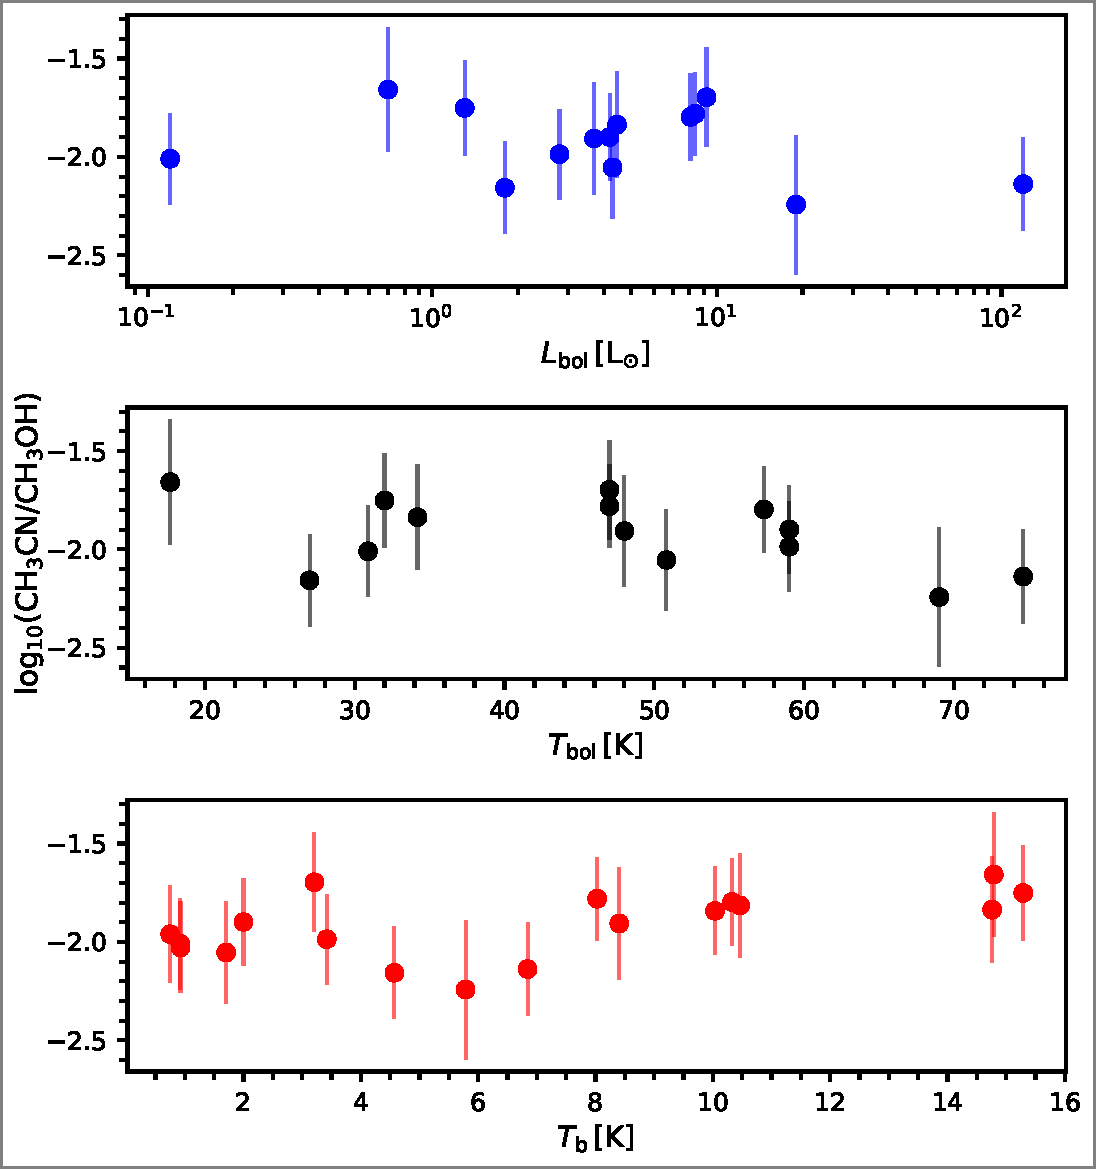
\includegraphics[width=0.47\textwidth]{ratio_ch3cn_ch3oh.pdf}
  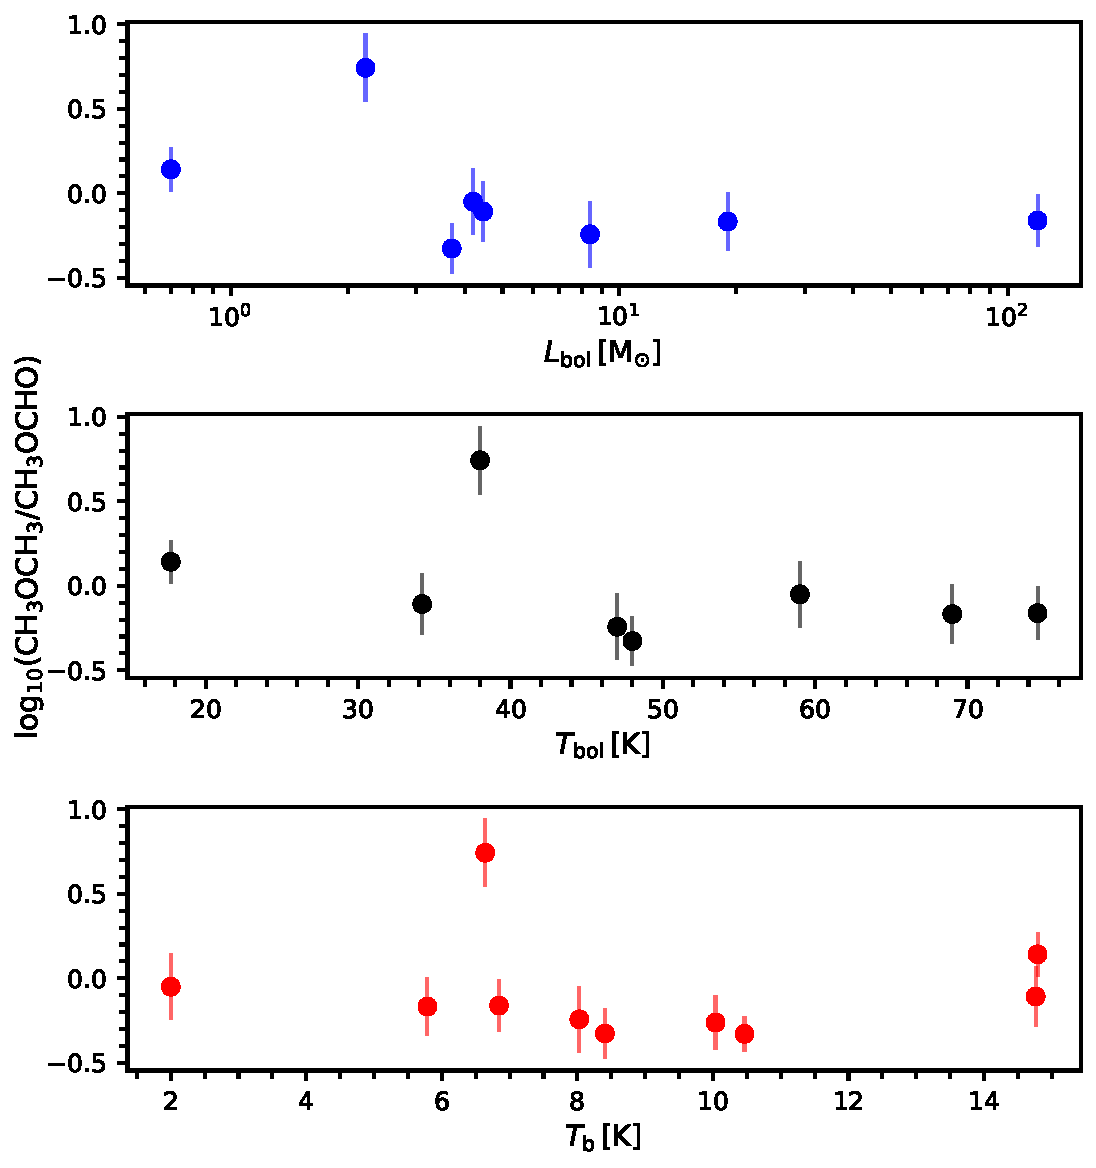
\includegraphics[width=0.47\textwidth]{ratio_ch3och3_ch3ocho.pdf}
  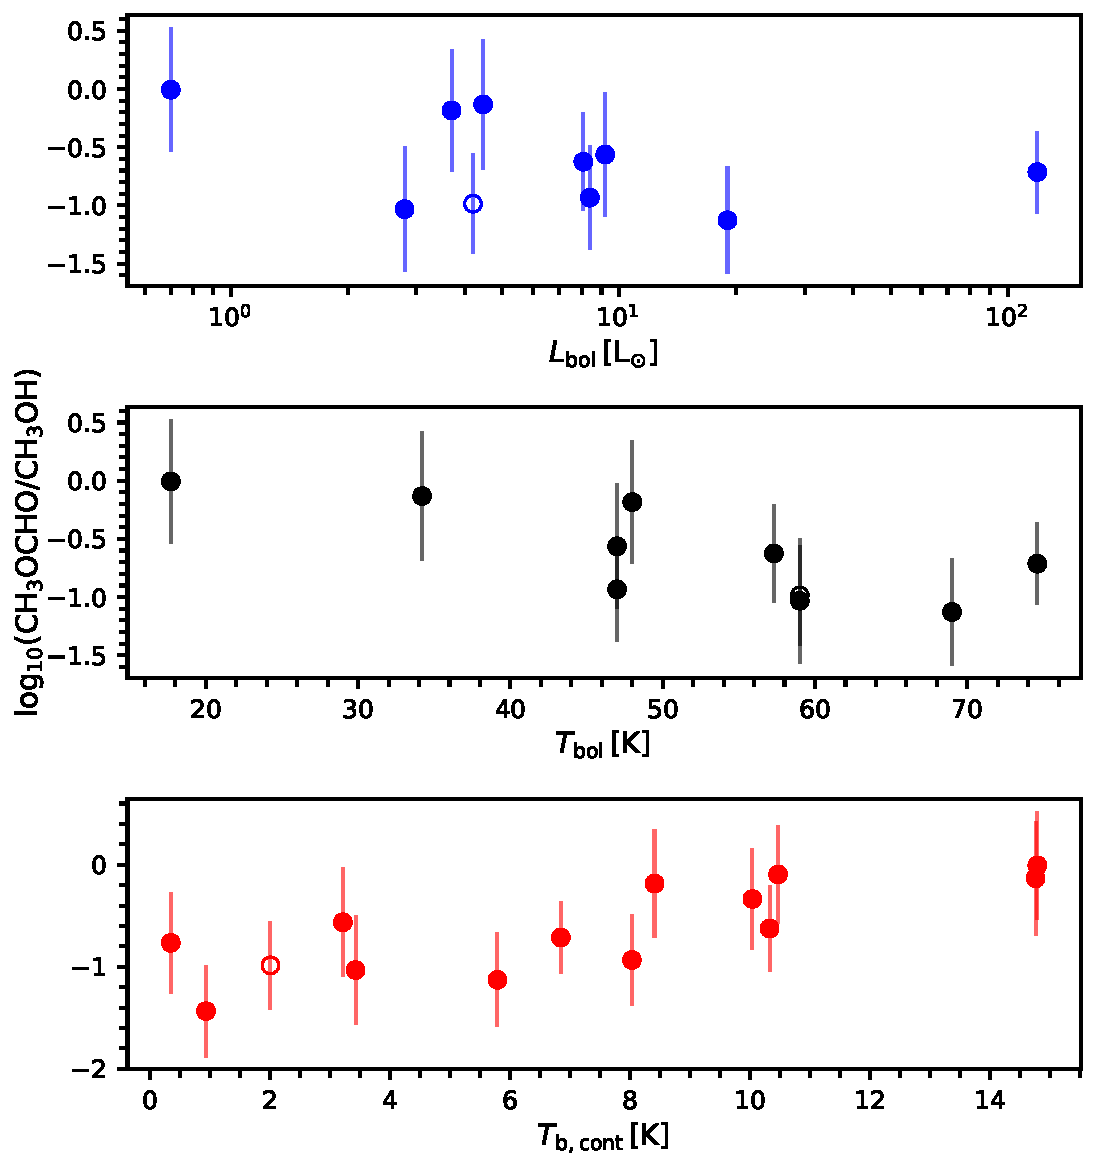
\includegraphics[width=0.47\textwidth]{ratio_ch3ocho_ch3oh.pdf}
  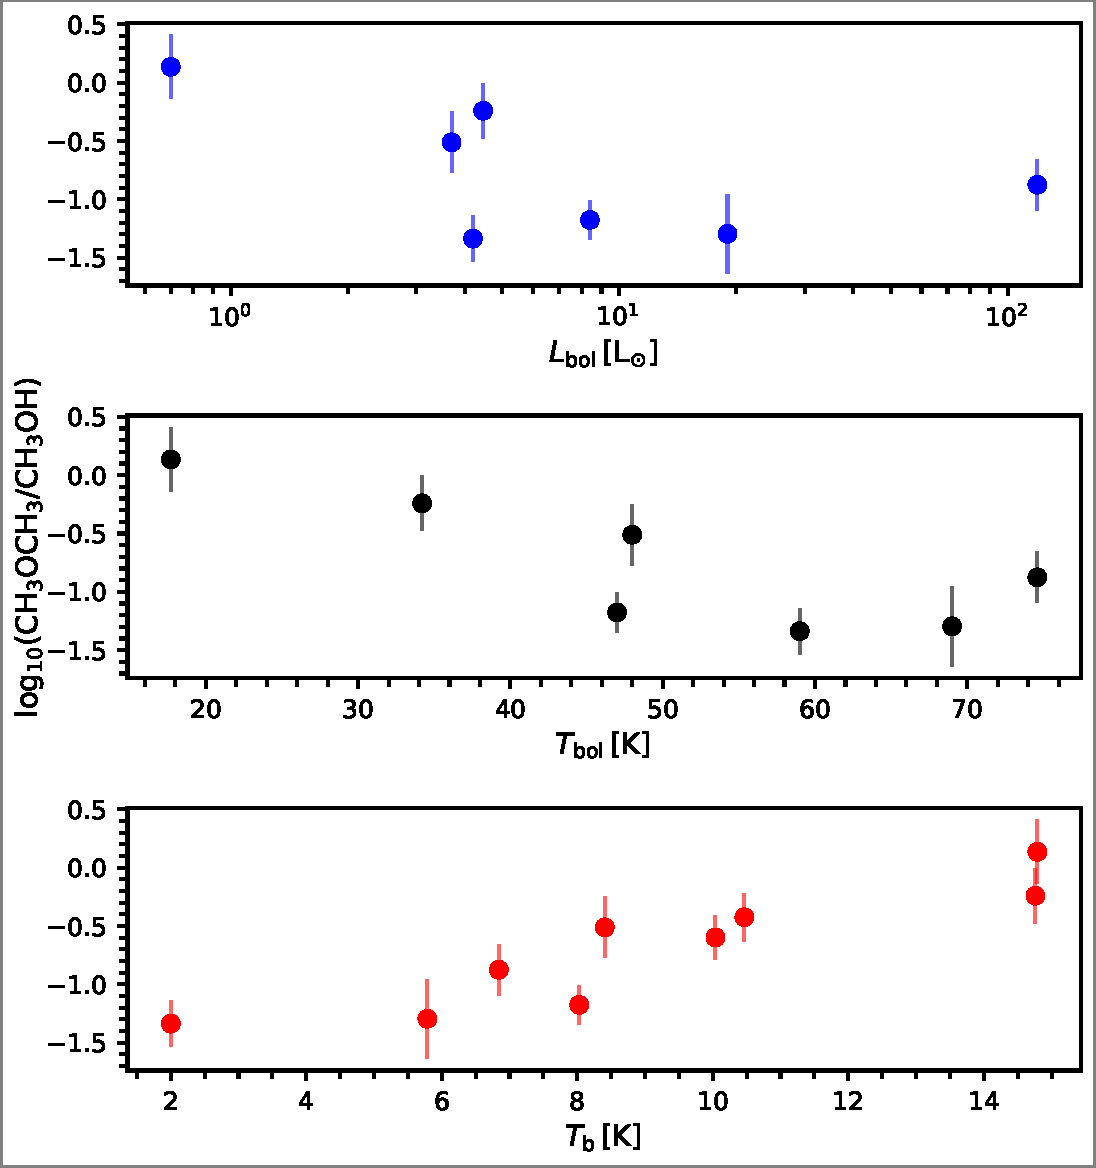
\includegraphics[width=0.47\textwidth]{ratio_ch3och3_ch3oh.pdf}
  \caption{Ratios of well-detected molecules, \methanol, \methylcyanide, \methylformate, and \dimethylether, as functions of \lbol\ (blue), \tbol\ (black), and \tbc\ (red).}
  \label{fig:ratios_indicators}
\end{figure*}

\textcolor{red}{size of COMs vs. Lbol}

\textcolor{pink}{No tight correlation with physical parameters.  --> hot corino emargence would not be the "determined story" in chemical evolution.  [refer figures 3/4]
[add some discussions of the position of hot corino sources]}

\subsection{The Abundance Ratios of O-bearing and N-bearing COMs}
\label{sec:ratios}

\begin{figure}[htbp!]
  \centering
  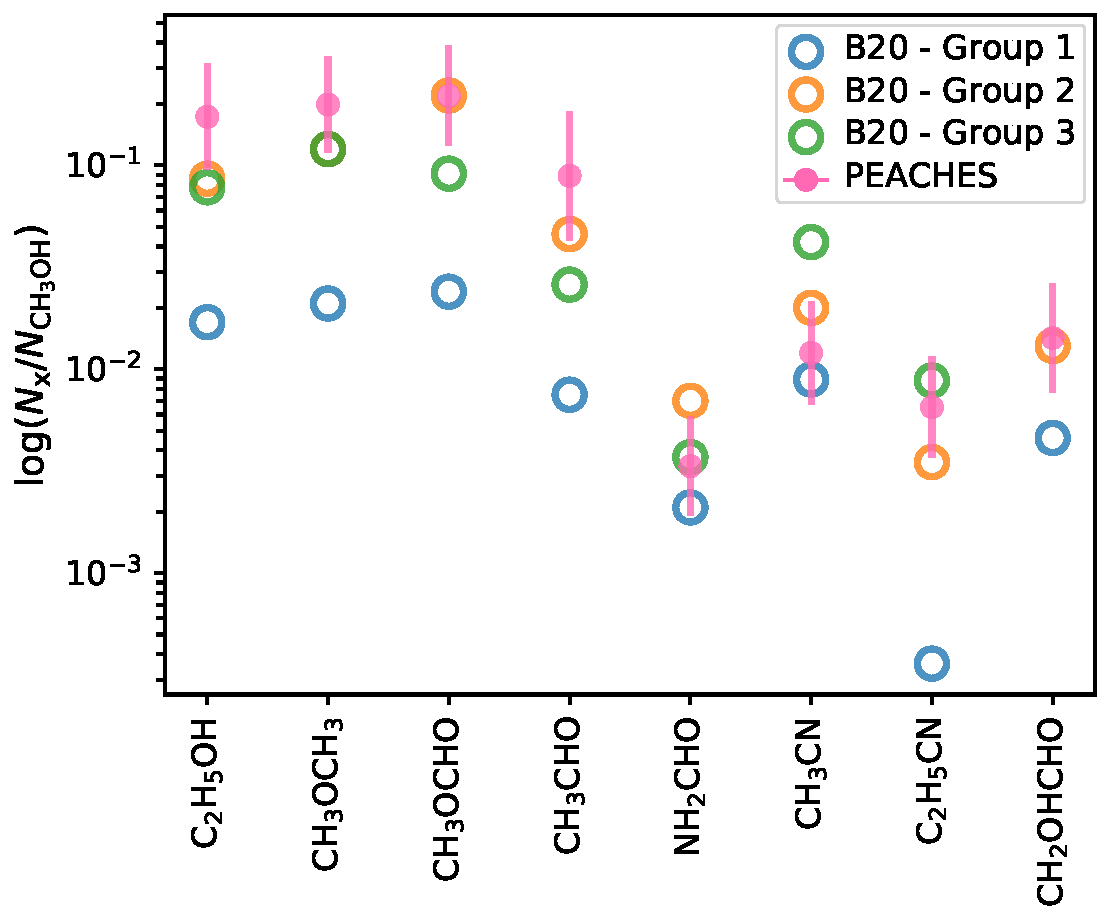
\includegraphics[width=0.47\textwidth]{ratios_survey.pdf}
  \caption{The ratios of the COMs commonly found in the PEACHES survey and the CALYPSO survey \citep{2020A&A...635A.198B}, which categorize their sample into three groups according to their COMs abundance to \methanol.  Group 3 has no detection of \glycolaldehyde.}
  \label{fig:ratio_calypso}
\end{figure}

- [please mention about abundance ratios C2H5CN, NH3CHO vs CH3OCH3 and CH3OCHO. and refer several papers discussed the O- and N difference.  such as in Orion KL and/or IRAS16293???] O- and N- difference might be enhanced in more complex species (?).

\subsection{Origin of the \methanol/\methylcyanide\ Correlation}
The tight correlation between \methanol\ and \methylcyanide\ is a striking finding of the PEACHES survey, while studies such as \citet{2017ApJ...841..120B,2020A&A...635A.198B} have shown a similar trend with fewer detections or larger scatter.  \citet{2020A&A...635A.198B} argue that this correlation between \methanol\ and \methylcyanide\ may not be due to chemistry because of the somewhat unrelated formation pathways of two molecules.  If the gas-phase chemistry is negligible for the production of \methanol\ and \methylcyanide, the tight correlation between \methanol\ and \methylcyanide\ suggests a similar abundance ratio of two molecules on the icy grains prior to being thermally desorbed.  Thus, the chemical processes that produce these two molecules may occur at a much shorter timescale compared to the dynamical scale of the protostellar evolution, hinting a universal chemistry of COMs at the warm protostellar envelope.  The tight correlation may also reflect a uniform elemental abundance of O and N in the Perseus molecular cloud before the star formation.

The compact emission of \methanol\ has a well known icy origin, where \methanol\ forms via the hydrogenation on the surface of dust grains.  \textcolor{red}{At cold temperature, the non-thermal desorption is thought to responsible for the production of \methanol.}  \methylcyanide\ can also form in gas-phase via radiative association (HCN $+$ CH$_3^+$ $\rightarrow$ CH$_3$CNH$^+$ $+$ $h\nu$) followed by the dissociative recombination of CH$_3$CNH$^+$ or on the grain surface.  The grain-surface reactions to form \methylcyanide\ can occur at cold temperature by the hydrogenation of CCN, which can form via
\begin{align}
  \text{C} + \text{CN} \rightarrow \text{CCN} \nonumber \\
  \text{C}_2 + \text{N} \rightarrow \text{CCN} \nonumber \\
  \text{(depleted)} \text{CCN}.
\end{align}
At warm temperature, \methylcyanide\ can form directly from reactions between radicals, CH$_3$ and CN.  For embedded protostars, the grain-surface reactions are thought to dominate the production of \methylcyanide; however, it remains unclear whether the cold phase or warm phase grain-surface pathway regulates the abundance of \methylcyanide.  

If we assume an icy grain origin for both \methanol\ and \methylcyanide, we can test the efficiency of the cold and warm phase pathways by comparing the ratio of \methylcyanide/\methanol\ toward the prestellar and protostellar sources.  \textcolor{red}{YLY: methanol must be released from dust grains via non-thermal reactions.  I recall there are some chemical reactions that can form methanol other than the grain-surface chemistry, perhaps some form of gas-phase chemistry, but don't know for sure now.}  At prestellar cores, [\methylcyanide/\methanol] are 0.28, 0.039, and 0.042 for TMC\,1 \citep{2016ApJS..225...25G}, L1521 E \citep{2019A&A...630A.136N}, and L1544 \citep{2019A&A...630A.136N}, respectively, all of which are higher than the ratio in our survey, 0.012$^{0.009}_{0.005}$.  The decreases of [\methylcyanide/\methanol] from prestellar to protostellar phase suggests that the warm phase grain-surface chemistry plays a rather insignificant role for the production of \methylcyanide\ and/or the gas-phase chemistry is more efficient at the cold phase to produce additional \methylcyanide.

\section{Conclusion}

\acknowledgements
Y.-L. Yang acknowledges the supports the JSPS Postdoctoral Fellowship from Japan Society for the Promotion of Science.  This paper makes use of the following ALMA data: ADS/JAO.ALMA\#2016.0.00391.S. ALMA is a partnership of ESO (representing its member states), NSF (USA) and NINS (Japan), together with NRC (Canada), MOST and ASIAA (Taiwan), and KASI (Republic of Korea), in cooperation with the Republic of Chile. The Joint ALMA Observatory is operated by ESO, AUI/NRAO and NAOJ.  The National Radio Astronomy Observatory is a facility of the National Science Foundation operated under cooperative agreement by Associated Universities, Inc.

\facilities{ALMA}

\software{astropy \citep{2018AJ....156..123A}, XCLASS \citep{2017A&A...598A...7M}, spectral-cube \citep{2016ascl.soft09017R}, CASA \citep{2007ASPC..376..127M}}

\appendix
\section{Catalogs for Molecular Data}
\label{sec:catalogs}
The spectroscopic data are taken from the Cologne Database of Molecular Spectroscopy (CDMS; \citealt{2001A&A...370L..49M,2005JMoSt.742..215M,2016JMoSp.327...95E}) and the Jet Propulsion Laboratory (JPL; \citealt{1998JQSRT..60..883P}).  Here we list only the references that cover the frequencies relevant to this study.  

For \methanol, the data were taken from \citet{2008JMoSp.251..305X}; for \dmethanol, the data were taken from \citet{2012JMoSp.280..119P}; for \tmethanol, the data were taken from \citet{1997JPCRD..26...17X}.  For \methylformate, the data were taken from \citet{2009JMoSp.255...32I}, which includes the data from \citet{1984ApJS...55..633P,1999ApJ...521..255O,2007JMoSp.246..158C,2008JMoSp.251..293M}.  For \acetaldehyde, the data were taken from \citet{1996JPCRD..25.1113K}.  For \dimethylether, the data were taken from \citet{2009A&A...504..635E}.  For \acetone, the data were taken from \citet{2002ApJS..142..145G}.  For CH$_{3}$C$^{15}$N, the data were taken from \citet{2009A&A...506.1487M} together with the data from \citet{1996ApJ...471.1067P}.  For gauche-\ethanol, the data were taken from \citet{2008JMoSp.251..394P} together with the data from \citet{1996JMoSp.175..246P}.  For \ethylcyanide, the data were compiled from \citet{1994ApJS...93..589P,2009ApJS..184..133B}.  For SO$_{2}$, the data were taken from \citet{2005JMoSp.232..213M} with additional data from \citet{1985JPCRD..14..395L,1985JMoSp.111...66H,1998JMoSp.191...17B}.


\newpage
\section{Identified Species and Transitions}
Table\,\ref{tbl:line_id} lists the species and their transitions identified from the PEACHES spectra.
\newpage
% \startlongtable
\begin{deluxetable*}{cccccc}
    \tabletypesize{\scriptsize}
    \tablecaption{Line Identification \label{tbl:line_id}}
    \tablewidth{\textwidth}
    \tablehead{\colhead{Frequency (MHz)} & \colhead{Transition\tablenotemark{a}} & 
               \colhead{log(Einstein-A)} & \colhead{$E_\text{u}$ (K)} & \colhead{$g_\text{u}$} & \colhead{Ref.}}
    \startdata
    \multicolumn{6}{c}{Ethynyl (CCH)} \\
    \hline
    262065.00 (0.05) & [3, 5/2, 3]\rt[2, 3/2, 2]\tablenotemark{b}   & $-$4.31 & 25.16  & 7  & CDMS \\
    262067.47 (0.05) & [3, 5/2, 2]\rt[2, 3/2, 1]\tablenotemark{b}   & $-$4.35 & 25.16  & 5  & CDMS \\
    262078.93 (0.02) & [3, 5/2, 2]\rt[2, 3/2, 2]\tablenotemark{b}   & $-$5.22 & 25.16  & 5  & CDMS \\
    \hline
    \multicolumn{6}{c}{Cyclopropenylidene (\cctht)} \\
    \hline
    244222.15 (0.01) & [3, 2, 1]\rt[2, 1, 2]                        & $-$4.23 & 18.17  & 21 & CDMS \\
    246557.77 (0.02) & [16, 10, 7]\rt[16, 9, 8]                     & $-$3.36 & 397.83 & 99 & CDMS \\
    260479.75 (0.02) & [5, 3, 2]\rt[4, 4, 1]                        & $-$3.79 & 44.72  & 33 & CDMS \\
    \hline
    \multicolumn{6}{c}{Methanol (\methanol\ $v_\text{t}=0$)} \\
    \hline
    243915.79 (0.01) & [5, 1, 4]\rt[4, 1, 3] A                      & $-$4.22 & 49.66  & 44 & CDMS \\
    246074.61 (0.02) & [20, 3, 17]\rt[20, 2, 18] A                  & $-$4.08 & 537.03 & 164& CDMS \\
    246873.30 (0.02) & [19, 3, 16]\rt[19, 2, 17] A                  & $-$4.08 & 490.65 & 156& CDMS \\
    261805.68 (0.01) & [2, 1, 1]\rt[1, 0, 1] E                      & $-$4.25 & 28.01  & 20 & CDMS \\
    \hline
    \multicolumn{6}{c}{Methanol (\tmethanol\ $v_\text{t}=0$)} \\
    \hline
    246426.12 (0.22) & [23, 4, 19]\rt[22, 5, 18]                    & $-$4.58 & 721.02 & 47 & CDMS \\
    247086.3 (0.5)   & [23, 3, 20]\rt[23, 2, 21] A$-$\rt\ A$+$      & $-$4.07 & 674.86 & 47 & CDMS \\
    259036.49 (0.17) & [17, 3, 15]\rt[17, 2, 16] A$+$\rt\ A$-$      & $-$4.04 & 396.48 & 35 & CDMS \\
    \hline
    \multicolumn{6}{c}{Methanol (\dmethanol\ $v_\text{t}=0$)} \\
    \hline
    243514.31 (0.01) & [9, 2, 8]\rt[10, 1, 10] o$_\text{1}$         & $-$5.17 & 131.85 & 19 & JPL  \\
    246973.11 (0.01) & [4, 1, 4]\rt[4, 1, 3] e$_\text{1}$           & $-$4.67 & 37.69  & 9  & JPL  \\
    260543.63 (0.01) & [3, 2, 1]\rt[3, 1, 2] o$_\text{1}$           & $-$4.65 & 48.34  & 7  & JPL  \\
    \hline
    \multicolumn{6}{c}{Methanol (\etmethanol\ $v_\text{t}=0$)} \\
    \hline
    246256.60 (0.04) & [11. 2. 10]\rt[10, 3, 7] A                   & $-$4.64 & 184.27 & 92 & CDMS \\
    \hline
    \multicolumn{6}{c}{Sulfur monoxide (\sosigma)} \\
    \hline
    258255.83 (0.01) & [\N, \J]$=$[6, 6]\rt[5, 5]                   & $-$3.67 & 56.50  & 13 & CDMS \\
    261843.72 (0.03) & [\N, \J]$=$[7, 6]\rt[6, 5]                   & $-$3.64 & 47.55  & 15 & CDMS \\
    \hline
    \multicolumn{6}{c}{Sulfur monoxide (\tfso)} \\
    \hline
    246663.47 (0.1)  & [\N, \J]$=$[5, 6]\rt[4, 5]                   & $-$3.74 & 49.89  & 11 & CDMS \\
    \hline
    \multicolumn{6}{c}{Sulfur dioxide (\sotwo)} \\
    \hline
    244254.22 (0.01) & [14, 0, 14]\rt[13, 1, 13]                    & $-$3.79 & 93.90  & 29 & CDMS \\
    \hline
    \multicolumn{6}{c}{Hydrogen cyanide (\htcn)} \\
    \hline
    259010.26 (0.01) & [\J, \F]$=$[3, 3]\rt[2, 3]                   & $-$4.07 & 24.86  & 7  & CDMS \\
    259011.55 (0.01) & [\J, \F]$=$[3, 2]\rt[2, 1]                   & $-$3.19 & 24.86  & 5  & CDMS \\
    259011.80 (0.01) & [\J, \F]$=$[3, 3]\rt[2, 2]                   & $-$3.16 & 24.86  & 7  & CDMS \\
    259011.86 (0.01) & [\J, \F]$=$[3, 4]\rt[2, 3]                   & $-$3.11 & 24.86  & 9  & CDMS \\
    259012.34 (0.01) & [\J, \F]$=$[3, 2]\rt[2, 3]                   & $-$5.46 & 24.86  & 5  & CDMS \\
    259013.89 (0.01) & [\J, \F]$=$[3, 2]\rt[2, 2]                   & $-$3.92 & 24.86  & 5  & CDMS \\
    \hline
    \multicolumn{6}{c}{Carbon Monosulfide (CS)} \\
    \hline
    244935.56 (0.01) & [\J]$=$[5]\rt[4]                             & $-$3.53 & 35.27  & 11 & CDMS \\
    \hline
    \multicolumn{6}{c}{Formaldehyde (HDCO)} \\
    \hline
    246924.6 (0.1)   & [4, 1, 4]\rt[3, 1, 3]                        & $-$3.40 & 37.60  & 9  & CDMS \\
    259034.9 (0.1)   & [4, 2, 2]\rt[3, 2, 1]                        & $-$3.44 & 62.86  & 9  & CDMS \\
    \hline
    \multicolumn{6}{c}{Methyl formate (\methylformate)} \\
    \hline
    245883.2 (0.1)   & [20, 13, 7]\rt[19, 13, 6] E                  & $-$3.89 & 235.98 & 82 & JPL  \\
    245885.2 (0.1)   & [20, 13, 7]\rt[19, 13, 6] A                  & $-$3.89 & 235.98 & 82 & JPL  \\
    245885.2 (0.1)   & [20, 13, 8]\rt[19, 13, 7] A                  & $-$3.89 & 235.98 & 82 & JPL  \\
    245903.7 (0.1)   & [20, 13, 8]\rt[19, 13, 7] E                  & $-$3.89 & 235.97 & 82 & JPL  \\
    246027.5 (0.1)   & [21, 2, 19]\rt[20, 3, 18] E                  & $-$4.63 & 139.85 & 86 & JPL  \\
    246038.9 (0.1)   & [21, 2, 19]\rt[20, 3, 18] A                  & $-$4.63 & 139.85 & 86 & JPL  \\
    246054.8 (0.1)   & [20, 12, 8]\rt[19, 12, 7] E                  & $-$3.84 & 219.43 & 82 & JPL  \\
    246060.8 (0.1)   & [20, 12, 8/9]\rt[19, 12, 7/8] A              & $-$3.84 & 219.43 & 82 & JPL  \\
    246076.9 (0.1)   & [20, 12, 9]\rt[19, 12, 8] E                  & $-$3.84 & 219.41 & 82 & JPL  \\
    246285.4 (0.1)   & [20, 11, 9]\rt[19, 11, 8] E                  & $-$3.80 & 204.21 & 82 & JPL  \\
    246295.1 (0.1)   & [20, 11, 10]\rt[19, 11, 9] A                 & $-$3.80 & 204.21 & 82 & JPL  \\
    246295.1 (0.1)   & [20, 11, 9]\rt[19, 11, 8] A                  & $-$3.80 & 204.21 & 82 & JPL  \\
    246308.3 (0.1)   & [20, 11, 10]\rt[19, 11, 9] E                 & $-$3.80 & 204.20 & 82 & JPL  \\
    246456.1 (0.1)   & [10, 5, 6]\rt[9, 4, 5] E                     & $-$5.52 & 49.09  & 42 & JPL  \\
    246600.0 (0.1)   & [20, 10, 10]\rt[19, 10, 9] E                 & $-$3.77 & 190.34 & 82 & JPL  \\
    246613.4 (0.1)   & [20, 10, 11]\rt[19, 10, 10] A                & $-$3.77 & 190.34 & 82 & JPL  \\
    246613.4 (0.1)   & [20, 10, 10]\rt[19, 10, 9] A                 & $-$3.77 & 190.34 & 82 & JPL  \\
    246623.2 (0.1)   & [20, 10, 11]\rt[19, 10, 10] E                & $-$3.77 & 190.34 & 82 & JPL  \\
    % 246630.0 (0.1)   & [35, 6, 30]\rt[35, 5, 31] A                  & $-$4.77 & 397.98 &142 & JPL  \\
    246660.5 (0.1)   & [10, 5, 6]\rt[9, 4, 5] A                     & $-$4.74 & 49.08  & 42 & JPL  \\
    246675.4 (0.1)   & [15, 4, 12]\rt[14, 3, 11] E                  & $-$4.93 & 81.85  & 62 & JPL  \\
    246683.5 (0.1)   & [15, 4, 12]\rt[14, 3, 11] A                  & $-$4.93 & 81.84  & 62 & JPL  \\
    246752.9 (0.1)   & [10, 5, 5]\rt[9, 4, 5] E                     & $-$4.90 & 49.10  & 42 & JPL  \\
    246891.6 (0.1)   & [19, 4, 15]\rt[18, 4, 14] E                  & $-$3.66 & 126.22 & 78 & JPL  \\
    246914.7 (0.1)   & [19, 4, 15]\rt[18, 4, 14] A                  & $-$3.66 & 126.22 & 78 & JPL  \\
    246945.7 (0.1)   & [10, 5, 6]\rt[9, 4, 6] E                     & $-$4.90 & 49.09  & 42 & JPL  \\
    247040.7 (0.1)   & [20, 9, 11]\rt[19, 9, 10] E                  & $-$3.74 & 177.83 & 82 & JPL  \\
    247044.1 (0.1)   & [21, 3, 19]\rt[20, 3, 18] E                  & $-$3.66 & 139.90 & 86 & JPL  \\
    247053.5 (0.1)   & [21, 3, 19]\rt[20, 3, 18] A                  & $-$3.66 & 139.89 & 86 & JPL  \\
    247057.3 (0.1)   & [20, 9, 12]\rt[19, 9, 11] A                  & $-$3.74 & 177.83 & 82 & JPL  \\
    247057.7 (0.1)   & [20, 9, 11]\rt[19, 9, 10] A                  & $-$3.74 & 177.83 & 82 & JPL  \\
    247063.7 (0.1)   & [20, 9, 12]\rt[19, 9, 11] E                  & $-$3.74 & 177.83 & 82 & JPL  \\
    247124.3 (0.1)   & [10, 5, 5]\rt[9, 4, 6] E                     & $-$4.74 & 49.08  & 42 & JPL  \\
    258275.0 (0.1)   & [21, 13, 8]\rt[20, 13, 7] E                  & $-$3.79 & 248.37 & 86 & JPL  \\
    258277.4 (0.1)   & [21, 13, 8]\rt[20, 13, 7] A                  & $-$3.79 & 248.37 & 86 & JPL  \\
    258277.4 (0.1)   & [21, 13, 9]\rt[20, 13, 8] A                  & $-$3.79 & 248.37 & 86 & JPL  \\
    259341.9 (0.1)   & [24, 0, 24]\rt[23, 1, 23] E                  & $-$4.37 & 158.23 & 98 & JPL  \\
    259342.0 (0.1)   & [24, 1, 24]\rt[23, 1, 23] E                  & $-$3.58 & 158.23 & 98 & JPL  \\
    259342.1 (0.1)   & [24, 0, 24]\rt[23, 0, 23] E                  & $-$3.58 & 158.23 & 98 & JPL  \\
    259342.3 (0.1)   & [24, 1, 24]\rt[23, 0, 23] E                  & $-$4.37 & 158.23 & 98 & JPL  \\
    259342.7 (0.1)   & [24, 0, 24]\rt[23, 1, 23] A                  & $-$4.37 & 158.22 & 98 & JPL  \\
    259342.9 (0.1)   & [24, 1, 24]\rt[23, 1, 23] A                  & $-$3.58 & 158.22 & 98 & JPL  \\
    259343.0 (0.1)   & [24, 0, 24]\rt[23, 0, 23] A                  & $-$3.58 & 158.22 & 98 & JPL  \\
    259343.2 (0.1)   & [24, 1, 24]\rt[23, 0, 23] A                  & $-$4.37 & 158.22 & 98 & JPL  \\
    261822.3 (0.1)   & [17, 10, 7]\rt[17, 9, 8] A                   & $-$4.73 & 156.63 & 70 & JPL  \\
    262088.2 (0.1)   & [16, 10, 6]\rt[16, 9, 7] A                   & $-$4.76 & 146.59 & 66 & JPL  \\
    262088.2 (0.1)   & [16, 10, 7]\rt[16, 9, 8] A                   & $-$4.76 & 146.59 & 66 & JPL  \\
    \hline
    \multicolumn{6}{c}{Methyl formate (\methylformatev)} \\
    \hline
    243511.5 (0.1)   & [20, 12, 8]\rt[19, 12, 7] E                  & $-$3.85 & 407.25 & 82 & JPL  \\
    245846.9 (0.1)   & [21, 3, 19]\rt[20, 3, 18] E                  & $-$3.66 & 326.30 & 86 & JPL  \\
    246106.8 (0.1)   & [20, 7, 14]\rt[19, 7, 13] A                  & $-$3.70 & 343.77 & 82 & JPL  \\
    246184.2 (0.1)   & [20, 8, 13]\rt[19, 8, 12] E                  & $-$3.72 & 353.27 & 82 & JPL  \\
    246187.0 (0.1)   & [21, 2, 19]\rt[20, 2, 18] A                  & $-$3.66 & 326.62 & 86 & JPL  \\
    246233.6 (0.1)   & [20, 7, 13]\rt[19, 7, 12] A                  & $-$3.70 & 343.79 & 82 & JPL  \\
    246274.9 (0.1)   & [20, 7, 13]\rt[19, 7, 12] E                  & $-$3.70 & 343.86 & 82 & JPL  \\
    246410.95 (0.01) & [10, 5, 5]\rt[9, 4, 6] A                     & $-$4.73 & 236.70 & 42 & JPL  \\
    246422.7 (0.1)   & [22, 1, 21]\rt[21, 2, 20] A                  & $-$4.51 & 330.43 & 90 & JPL  \\
    246461.2 (0.1)   & [22, 2, 21]\rt[21, 2, 20] A                  & $-$3.65 & 330.43 & 90 & JPL  \\
    246488.4 (0.1)   & [22, 1, 21]\rt[21, 1, 20] A                  & $-$3.65 & 330.43 & 90 & JPL  \\
    246562.9 (0.1)   & [21, 2, 19]\rt[20, 2, 18] E                  & $-$3.66 & 326.24 & 86 & JPL  \\
    246706.5 (0.1)   & [22, 2, 21]\rt[21, 2, 20] E                  & $-$3.65 & 329.89 & 90 & JPL  \\
    246731.7 (0.1)   & [22, 1, 21]\rt[21, 1, 20] E                  & $-$3.65 & 329.89 & 90 & JPL  \\
    246985.2 (0.1)   & [20, 6, 15]\rt[19, 6, 14] A                  & $-$3.68 & 335.37 & 82 & JPL  \\
    259003.9 (0.1)   & [21, 7, 14]\rt[20, 7, 13] A                  & $-$3.63 & 356.22 & 86 & JPL  \\
    259025.8 (0.1)   & [21, 7, 14]\rt[20, 7, 13] E                  & $-$3.63 & 356.29 & 86 & JPL  \\
    260479.6 (0.1)   & [44, 9, 36]\rt[44, 8, 37] A                  & $-$4.59 & 828.74 & 178& JPL  \\
    \hline
    \multicolumn{6}{c}{Dimethyl ether (\dimethylether)} \\
    \hline
    246499.29 (0.01) & [37, 6, 31]\rt[37, 5, 12] AA                 & $-$4.01 & 693.72 & 750& CDMS \\
    246505.09 (0.01) & [37, 6, 31]\rt[37, 5, 12] AE                 & $-$4.01 & 693.72 & 450& CDMS \\
    246505.09 (0.01) & [37, 6, 31]\rt[37, 5, 12] EA                 & $-$4.01 & 693.72 & 300& CDMS \\
    246697.43 (0.01) & [27, 4, 23]\rt[26, 5, 21] AA                 & $-$4.70 & 367.61 & 330& CDMS \\
    246697.87 (0.01) & [27, 4, 23]\rt[26, 5, 21] EE                 & $-$4.70 & 367.61 & 880& CDMS \\
    246698.31 (0.01) & [27, 4, 23]\rt[26, 5, 21] AE                 & $-$4.70 & 367.61 & 110& CDMS \\
    246698.31 (0.01) & [27, 4, 23]\rt[26, 5, 21] EA                 & $-$4.70 & 367.61 & 220& CDMS \\
    259305.22 (0.01) & [33, 3, 31]\rt[34, 6, 28] AA                 & $-$6.61 & 563.02 & 670& CDMS \\
    259308.39 (0.01) & [33, 3, 31]\rt[34, 6, 28] AE                 & $-$6.61 & 563.02 & 402& CDMS \\
    259308.39 (0.01) & [33, 3, 31]\rt[34, 6, 28] EA                 & $-$6.61 & 563.02 & 268& CDMS \\
    259309.47 (0.01) & [17, 5, 12]\rt[17, 4, 13] AE                 & $-$4.06 & 174.54 & 210& CDMS \\
    259309.76 (0.01) & [17, 5, 12]\rt[17, 4, 13] EA                 & $-$4.06 & 174.54 & 140& CDMS \\
    259311.95 (0.01) & [17, 5, 12]\rt[17, 4, 13] EE                 & $-$4.06 & 174.54 & 560& CDMS \\
    259314.28 (0.01) & [17, 5, 12]\rt[17, 4, 13] AA                 & $-$4.06 & 174.54 & 350& CDMS \\
    \hline
    \multicolumn{6}{c}{Acetone (\acetone)} \\
    \hline
    244218.91 (0.01) & [20, 5, 15]\rt[19, 6, 14] AE                 & $-$3.32 & 139.69 & 82 & JPL \\
    244218.91 (0.01) & [20, 6, 15]\rt[19, 5, 14] AE                 & $-$3.32 & 139.69 & 250& JPL \\
    244218.92 (0.01) & [20, 5, 15]\rt[19, 6, 14] EA                 & $-$3.32 & 139.69 & 160& JPL \\
    244218.92 (0.01) & [20, 6, 15]\rt[19, 5, 14] EA                 & $-$3.32 & 139.69 & 160& JPL \\
    245831.34 (0.09) & [13, 10, 3]\rt[12, 9, 4] EE                  & $-$3.80 & 77.84  & 432& JPL \\ 
    246400.99 (0.05) & [34, 7, 28]\rt[34, 5, 29] EE                 & $-$4.17 & 364.98 &1100& JPL \\
    246400.99 (0.05) & [34, 6, 28]\rt[34, 5, 29] EE                 & $-$4.03 & 364.98 &1100& JPL \\
    246400.99 (0.05) & [34, 7, 28]\rt[34, 6, 29] EE                 & $-$4.03 & 364.98 &1100& JPL \\
    246400.99 (0.05) & [34, 6, 28]\rt[34, 6, 29] EE                 & $-$4.17 & 364.98 &1100& JPL \\
    246404.27 (0.01) & [22, 3, 19]\rt[21, 4, 18] AE                 & $-$3.23 & 149.62 & 90 & JPL \\
    246404.27 (0.01) & [22, 4, 19]\rt[21, 3, 18] AE                 & $-$3.23 & 149.62 & 270& JPL \\
    246404.29 (0.01) & [22, 3, 19]\rt[21, 4, 18] EA                 & $-$3.23 & 149.62 & 180& JPL \\
    246404.29 (0.01) & [22, 4, 19]\rt[21, 3, 18] EA                 & $-$3.23 & 149.62 & 180& JPL \\
    246450.40 (0.01) & [22, 4, 19]\rt[21, 3, 18] EE                 & $-$3.23 & 149.57 & 720& JPL \\
    246450.40 (0.01) & [22, 3, 19]\rt[21, 3, 18] EE                 & $-$5.09 & 149.57 & 720& JPL \\
    246450.40 (0.01) & [22, 3, 19]\rt[21, 4, 18] EE                 & $-$3.24 & 149.57 & 720& JPL \\
    246450.40 (0.01) & [22, 4, 19]\rt[21, 4, 18] EE                 & $-$4.92 & 149.57 & 720& JPL \\
    246496.17 (0.46) & [25, 14, 12]\rt[24, 15, 9] AE                & $-$5.01 & 257.11 & 100& JPL \\
    246496.47 (0.02) & [22, 3, 19]\rt[21, 4, 18] AA                 & $-$3.23 & 149.51 & 270& JPL \\
    246496.47 (0.02) & [22, 4, 19]\rt[21, 3, 18] AA                 & $-$3.23 & 149.51 & 450& JPL \\
    246714.12 (0.05) & [9, 8, 1]\rt[8, 5, 4] EA                     & $-$5.84 & 40.59  & 76 & JPL \\
    246714.94 (0.05) & [32, 4, 28]\rt[32, 4, 29] EA                 & $-$3.97 & 305.61 & 260& JPL \\
    246714.94 (0.05) & [32, 5, 28]\rt[32, 3, 29] EA                 & $-$3.97 & 305.61 & 260& JPL \\
    246715.04 (0.05) & [32, 5, 28]\rt[32, 4, 29] AE                 & $-$3.97 & 305.61 & 390& JPL \\
    246715.04 (0.05) & [32, 4, 28]\rt[32, 3, 29] EA                 & $-$3.97 & 305.61 & 130& JPL \\
    246719.92 (0.04) & [33, 6, 28]\rt[33, 4, 29] EE                 & $-$5.62 & 344.85 &1100& JPL \\
    246719.92 (0.04) & [33, 5, 28]\rt[33, 4, 29] EE                 & $-$3.87 & 344.85 &1100& JPL \\
    246719.92 (0.04) & [33, 6, 28]\rt[33, 5, 29] EE                 & $-$3.87 & 344.85 &1100& JPL \\
    246719.92 (0.04) & [33, 5, 28]\rt[33, 5, 29] EE                 & $-$5.61 & 344.85 &1100& JPL \\
    261818.11 (0.01) & [20, 7, 13]\rt[19, 8, 12] EA                 & $-$3.31 & 151.17 & 160& JPL \\
    261818.17 (0.01) & [20, 7, 13]\rt[19, 8, 12] AE                 & $-$3.31 & 151.17 & 82 & JPL \\
    261819.09 (0.01) & [20, 8, 13]\rt[19, 7, 12] EA                 & $-$3.31 & 151.17 & 160& JPL \\
    261819.17 (0.01) & [20, 8, 13]\rt[19, 7, 12] AE                 & $-$3.31 & 151.17 & 250& JPL \\
    \hline
    \multicolumn{6}{c}{Methyl cyanide (\methylcyanide)} \\
    \hline
    257507.56 (0.01) & [\N, \K]$=$[14, 2]\rt[13, 2]                 & $-$3.00 & 121.28 & 58 & JPL \\
    257522.43 (0.01) & [\N, \K]$=$[14, 1]\rt[13, 1]                 & $-$2.99 & 99.84  & 58 & JPL \\
    257527.38 (0.01) & [\N, \K]$=$[14, 0]\rt[13, 0]                 & $-$2.99 & 92.70  & 58 & JPL \\
    \hline
    \multicolumn{6}{c}{Acetaldehyde (\acetaldehyde\ $v_\text{t}=0$)} \\
    \hline
    246330.73 (0.01) & [15, 3, 13]\rt[15, 2, 14] A                  & $-$4.29 & 131.49 & 62 & JPL \\
    260530.40 (0.01) & [14, 1, 14]\rt[13, 1, 13] E                  & $-$3.20 & 96.39  & 58 & JPL \\
    260544.02 (0.01) & [14, 1, 14]\rt[13, 1, 13] A                  & $-$3.20 & 96.32  & 58 & JPL \\
    260547.46 (2.07) & [9, 4, 5]\rt[9, 3, 7] E, $v_\text{t}=2$      & $-$6.06 & 456.38 & 38 & JPL \\
    \hline
    \multicolumn{6}{c}{gauche-Ethanol ($g$-\ethanol)} \\
    \hline
    246414.76 (0.05) & [14, 3, 11]\rt[13, 3, 10] $v_\text{t}=0$\rt0 & $-$3.89 & 155.72 & 29 & JPL \\
    246524.28 (0.01) & [13, 2, 12]\rt[12, 1, 12] $v_\text{t}=0$\rt1 & $-$4.50 & 136.95 & 27 & JPL \\
    246658.18 (0.01) & [32, 5, 28]\rt[32, 4, 29] $v_\text{t}=0$\rt0 & $-$6.33 & 527.94 & 65 & JPL \\
    246662.98 (0.01) & [4, 2, 3]\rt[3, 1, 3] $v_\text{t}=1$\rt0     & $-$4.36 & 74.77  & 9  & JPL \\
    259322.64 (0.01) & [14, 3, 11]\rt[13, 2, 11] $v_\text{t}=0$\rt1 & $-$4.39 & 155.72 & 29 & JPL \\
    260457.73 (0.01) & [15. 4. 12]\rt[14, 4, 11] $v_\text{t}=1$\rt1 & $-$3.83 & 181.10 & 31 & JPL \\
    \hline
    \multicolumn{6}{c}{trans-Ethanol (\ethanol)} \\
    \hline
    246663.62 (0.05) & [24, 1, 23]\rt[24, 0, 24]                    & $-$3.73 & 252.35 & 49 & JPL \\
    261815.99 (0.05) & [28, 3, 26]\rt[28, 2, 27]                    & $-$3.96 & 350.98 & 57 & JPL \\
    \hline
    \multicolumn{6}{c}{Glycolaldehyde ($cis$-\glycolaldehyde)} \\
    \hline
    246773.09 (0.02) & [30, 2, 28]\rt[30, 1, 29]                    & $-$4.04 & 252.68 & 61 & CDMS \\
    246778.28 (0.02) & [30, 3, 28]\rt[30, 2, 29]                    & $-$4.04 & 252.68 & 61 & CDMS \\
    262056.78 (0.01) & [25, 2, 24]\rt[24, 1, 23]                    & $-$3.34 & 158.25 & 51 & CDMS \\
    261795.48 (0.01) & [25, 11, 14]\rt[25, 10, 15]                  & $-$3.57 & 254.23 & 51 & CDMS \\
    261798.96 (0.01) & [25, 11, 15]\rt[25, 10, 16]                  & $-$3.57 & 254.23 & 51 & CDMS \\
    \hline
    \multicolumn{6}{c}{Methyl cyanide (\dmethylcyanide)} \\
    \hline
    259315.51 (0.01) & [15, 1, 15]\rt[14, 1, 14]                    & $-$2.82 & 104.97 & 31 & CDMS \\
    260523.05 (0.01) & [15, 2, 13]\rt[14, 2, 12]                    & $-$2.82 & 121.60 & 31 & CDMS \\
    \hline
    \multicolumn{6}{c}{Ethyl cyanide (\ethylcyanide)} \\
    \hline
    246268.74 (0.01) & [27, 2, 25]\rt[26, 2, 24]                    & $-$2.90 & 169.80 & 55 & CDMS \\
    246421.92 (0.01) & [28, 2, 27]\rt[27, 2, 26]                    & $-$2.90 & 177.26 & 57 & CDMS \\
    246548.70 (0.01) & [27, 3, 24]\rt[26, 3, 23]                    & $-$2.90 & 174.06 & 55 & CDMS \\
    260535.69 (0.05) & [29, 5, 25]\rt[28, 5, 24]                    & $-$2.84 & 215.06 & 59 & CDMS \\
    \hline
    \multicolumn{6}{c}{Formamide (\formamide)} \\
    \hline
    243521.04 (0.01) & [12, 1, 12]\rt[11, 1, 11]                    & $-$2.98 & 79.19  & 25 & CDMS \\
    \hline
    \multicolumn{6}{c}{Formic acid (\tcooh)} \\
    \hline
    262103.48 (0.01) & [12, 0, 12]\rt[11, 0, 11]                    & $-$3.69 & 82.77  & 25 & CDMS \\
    \enddata
    \tablenotetext{a}{The typical quantum numbers are listed as [\J, \Ka, \Kc] unless specified.}
    \tablenotetext{b}{The quantum numbers are [\N, \J, \F]}
\end{deluxetable*}

\section{Intensity maps of \methanol, \methylcyanide, \methylformate, and \dimethylether}
\label{sec:coms_maps}
\newpage\begin{figure*}[htbp!]
  \centering
  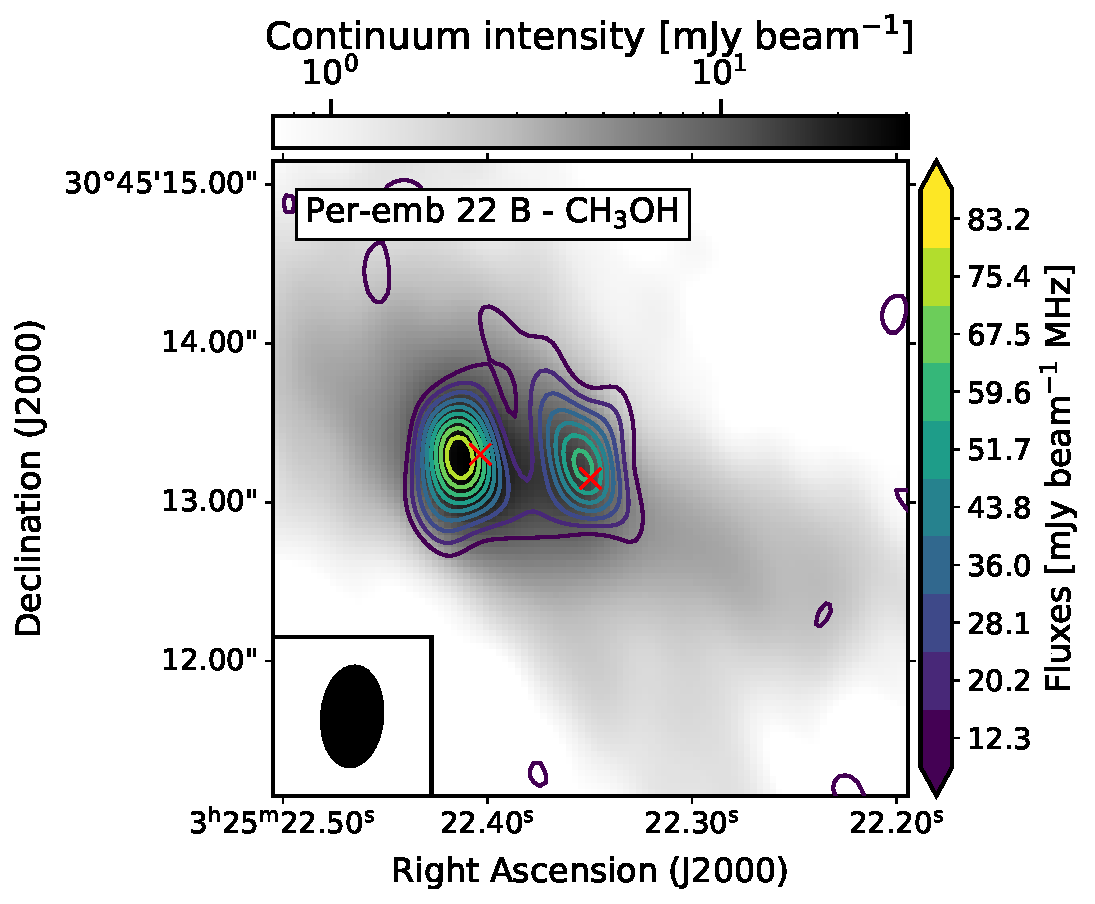
\includegraphics[width=0.24\textwidth]{/Users/yaolun/1d_spectra/extractions/moment0/subset/Set1_ID03_2_CH3OH_243915.pdf}
  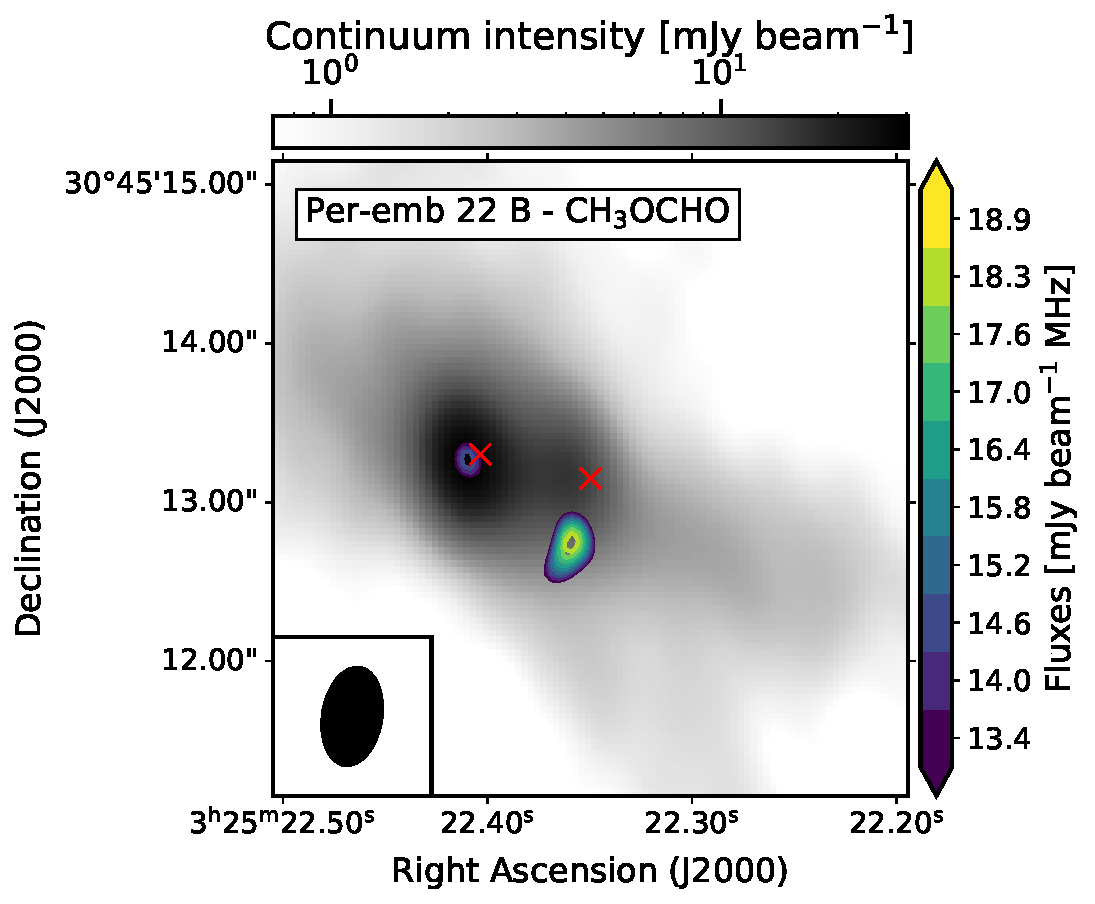
\includegraphics[width=0.24\textwidth]{/Users/yaolun/1d_spectra/extractions/moment0/subset/Set1_ID03_2_CH3OCHO_259342.pdf}
  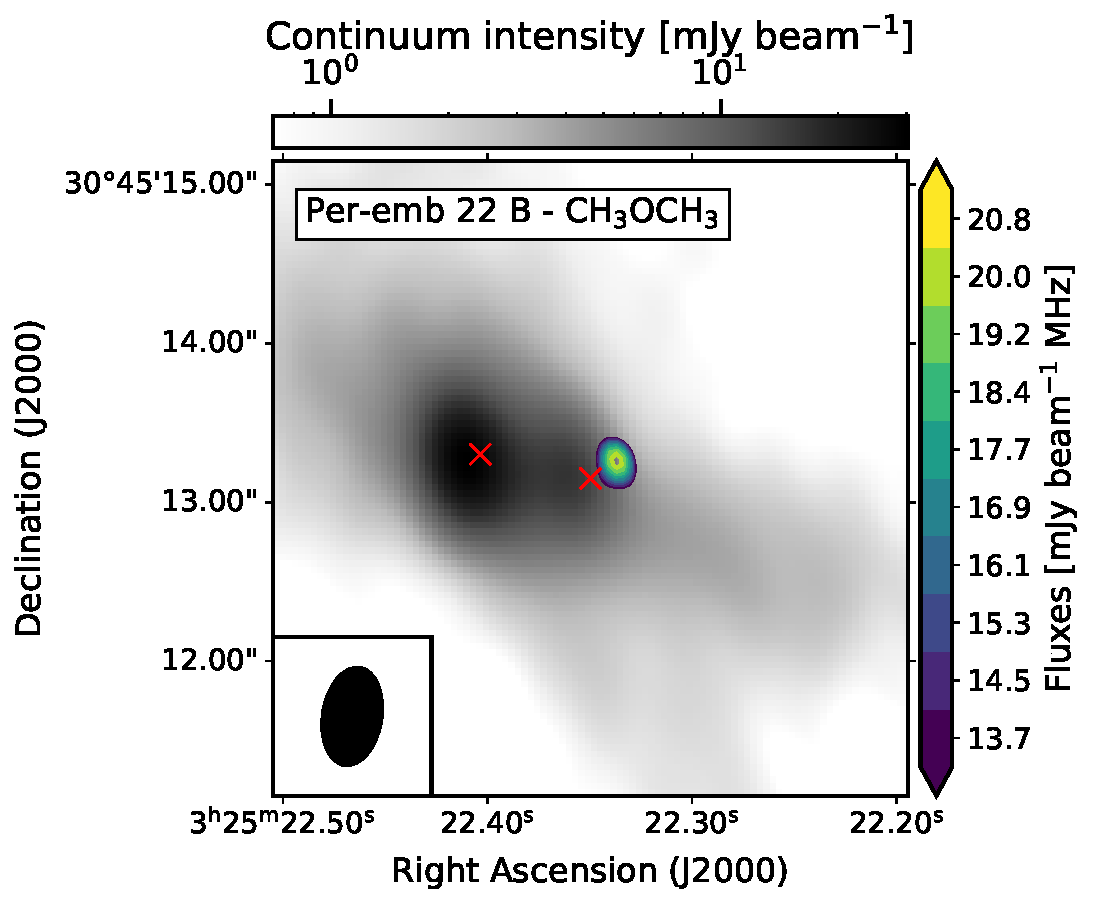
\includegraphics[width=0.24\textwidth]{/Users/yaolun/1d_spectra/extractions/moment0/subset/Set1_ID03_2_CH3OCH3_259311.pdf}
  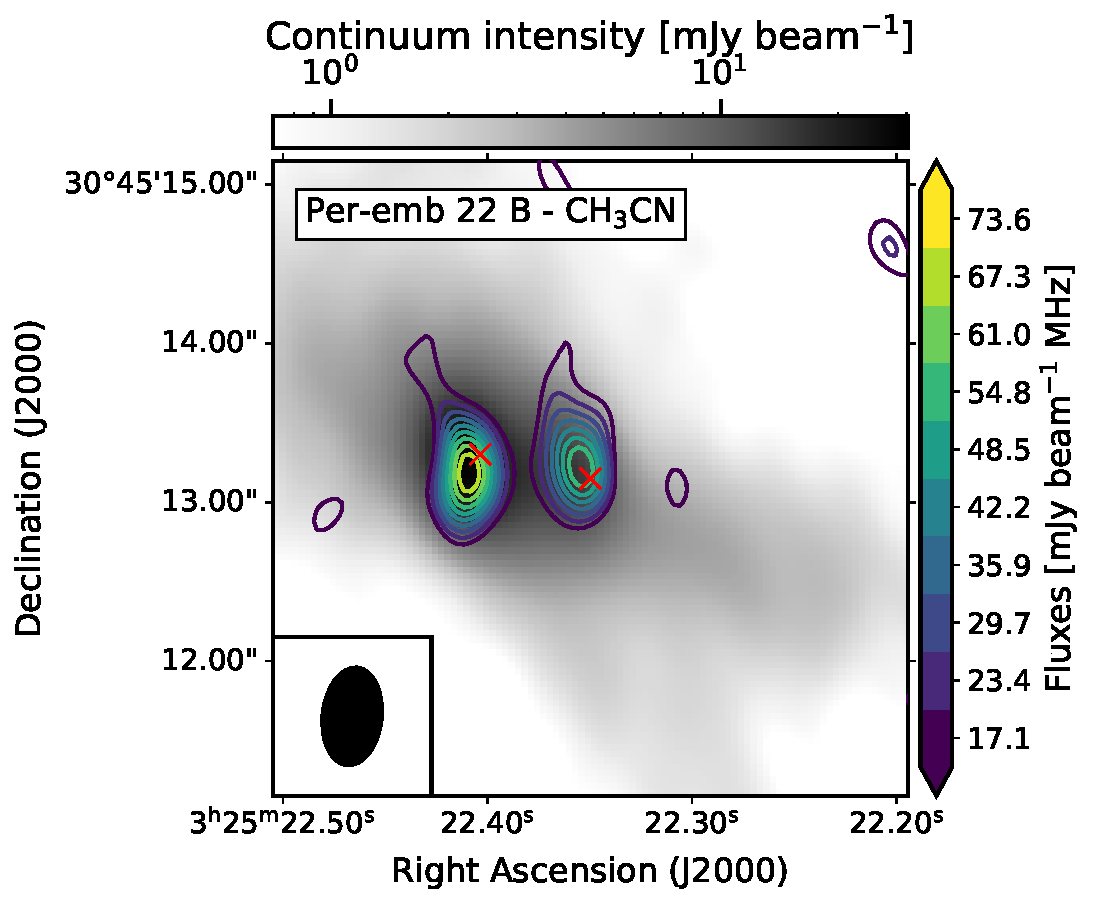
\includegraphics[width=0.24\textwidth]{/Users/yaolun/1d_spectra/extractions/moment0/subset/Set1_ID03_2_CH3CN_257527.pdf}
  \\
  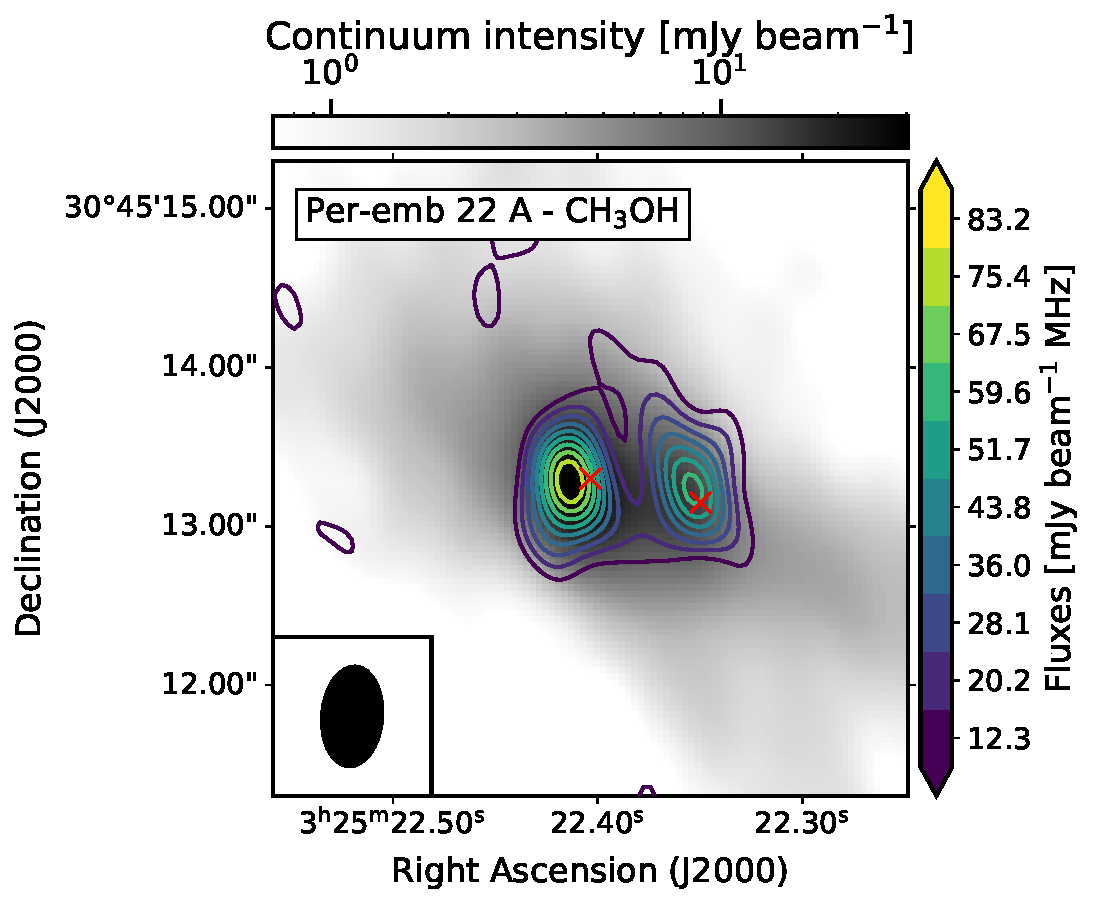
\includegraphics[width=0.24\textwidth]{/Users/yaolun/1d_spectra/extractions/moment0/subset/Set1_ID03_CH3OH_243915.pdf}
  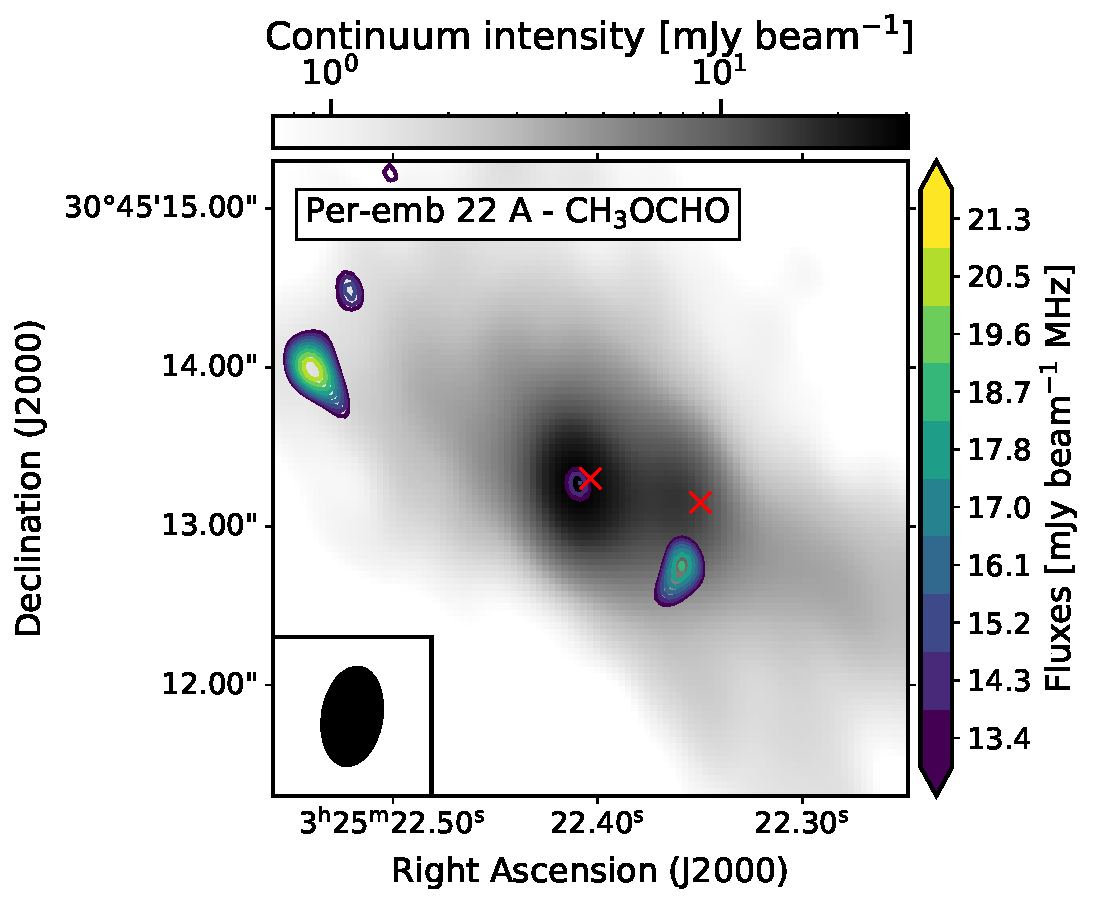
\includegraphics[width=0.24\textwidth]{/Users/yaolun/1d_spectra/extractions/moment0/subset/Set1_ID03_CH3OCHO_259342.pdf}
  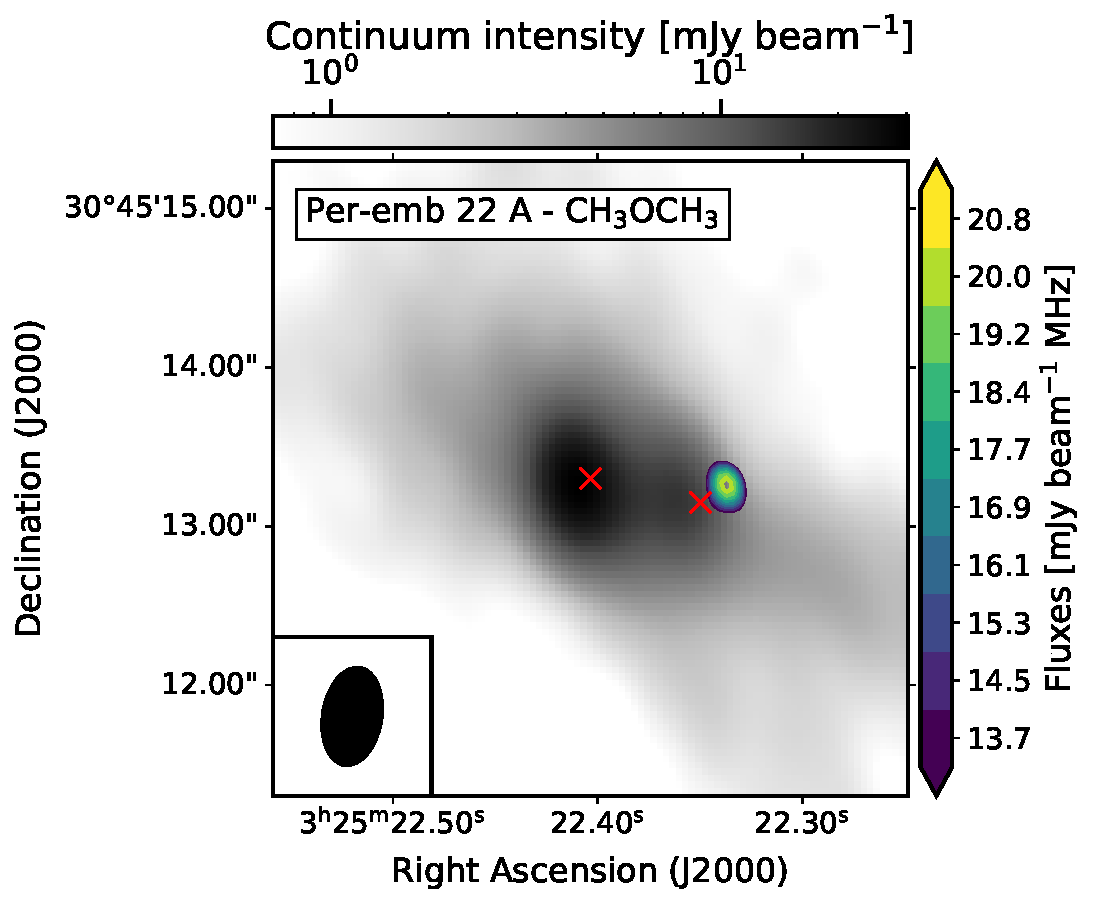
\includegraphics[width=0.24\textwidth]{/Users/yaolun/1d_spectra/extractions/moment0/subset/Set1_ID03_CH3OCH3_259311.pdf}
  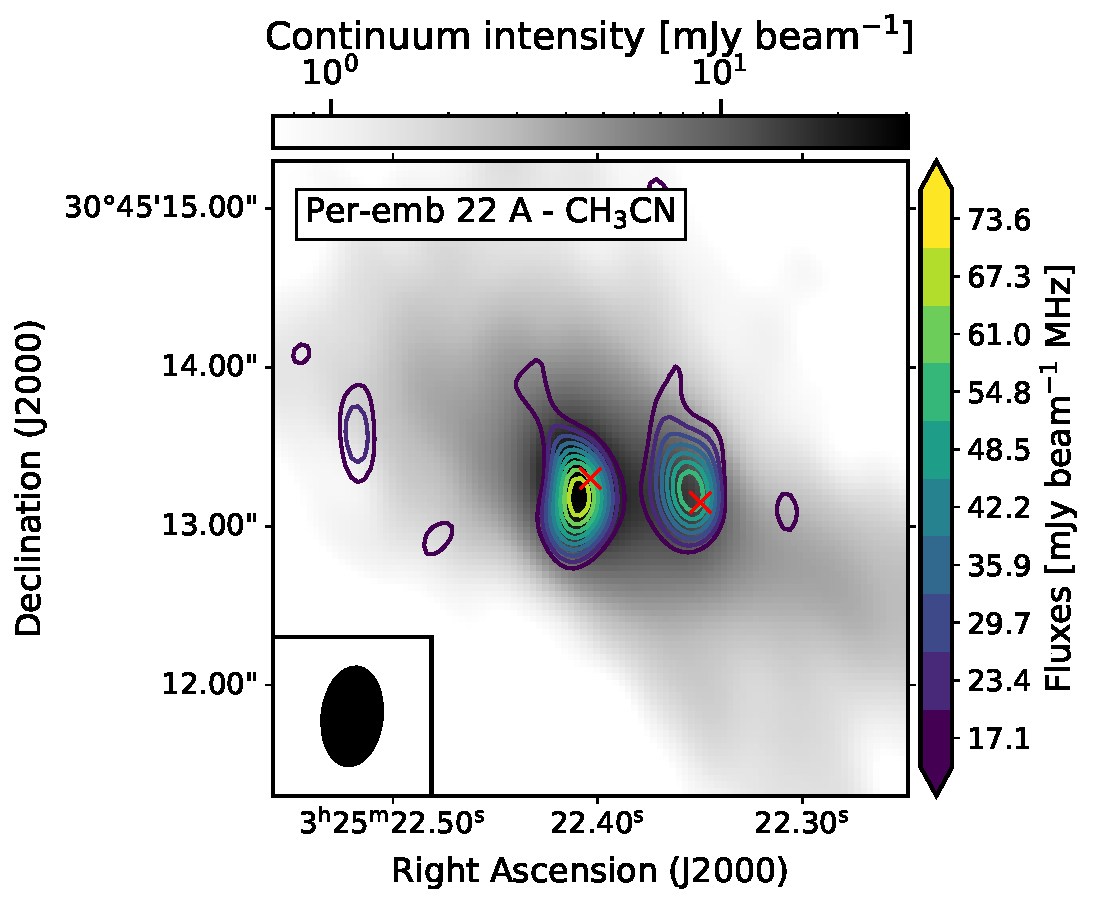
\includegraphics[width=0.24\textwidth]{/Users/yaolun/1d_spectra/extractions/moment0/subset/Set1_ID03_CH3CN_257527.pdf}
  \\
  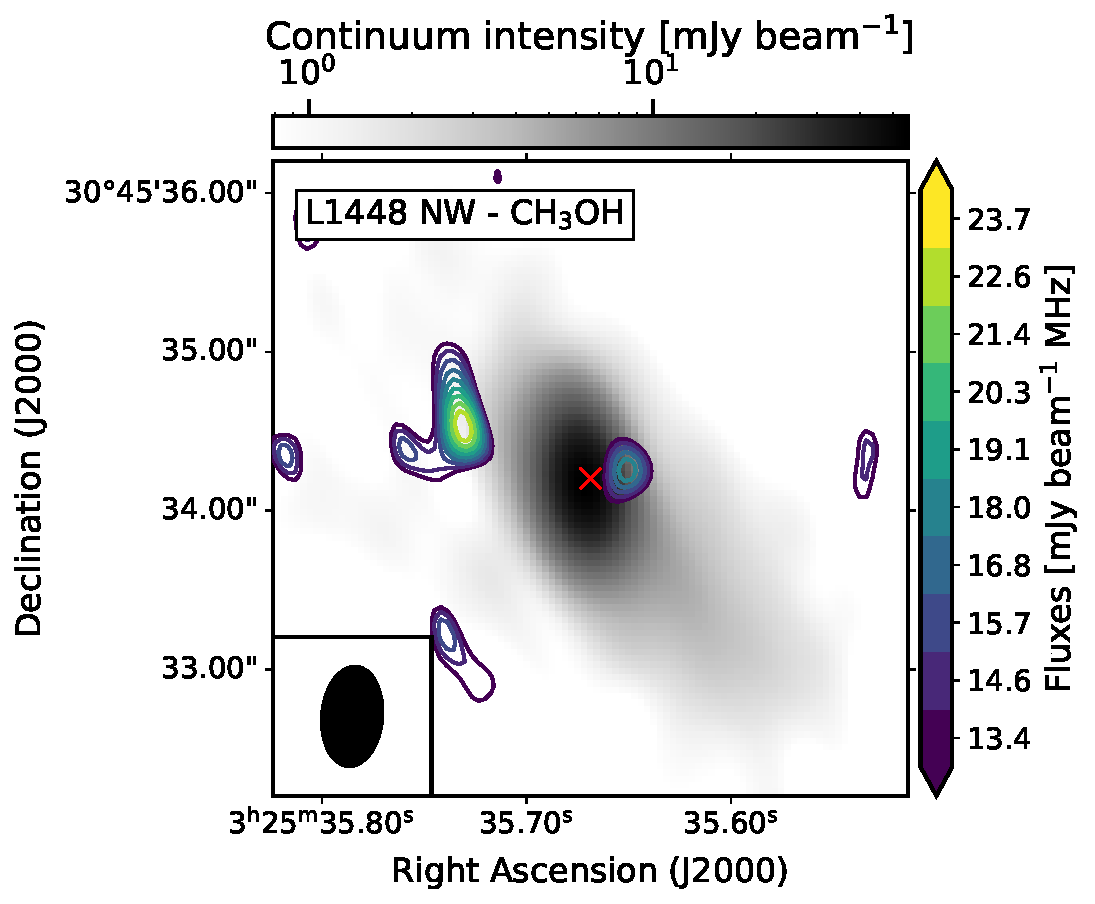
\includegraphics[width=0.24\textwidth]{/Users/yaolun/1d_spectra/extractions/moment0/subset/Set1_ID00_CH3OH_243915.pdf}
  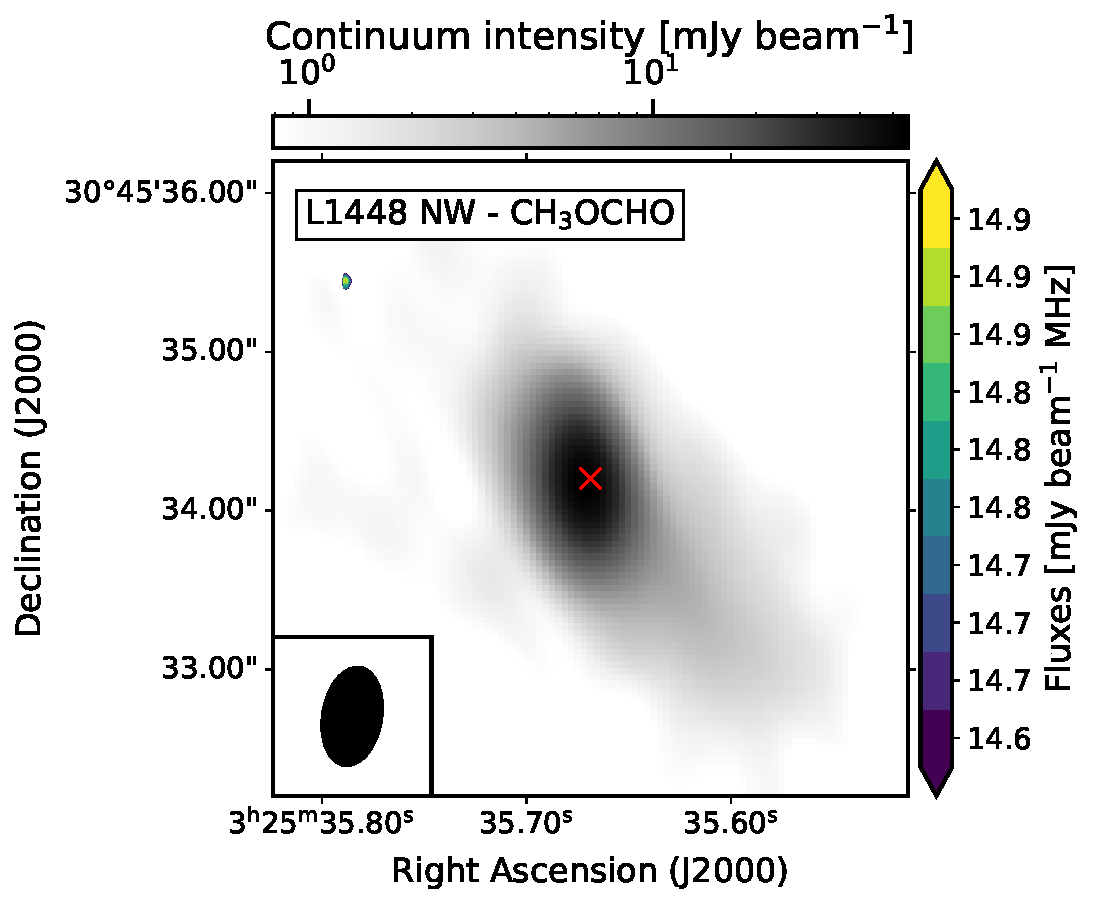
\includegraphics[width=0.24\textwidth]{/Users/yaolun/1d_spectra/extractions/moment0/subset/Set1_ID00_CH3OCHO_259342.pdf}
  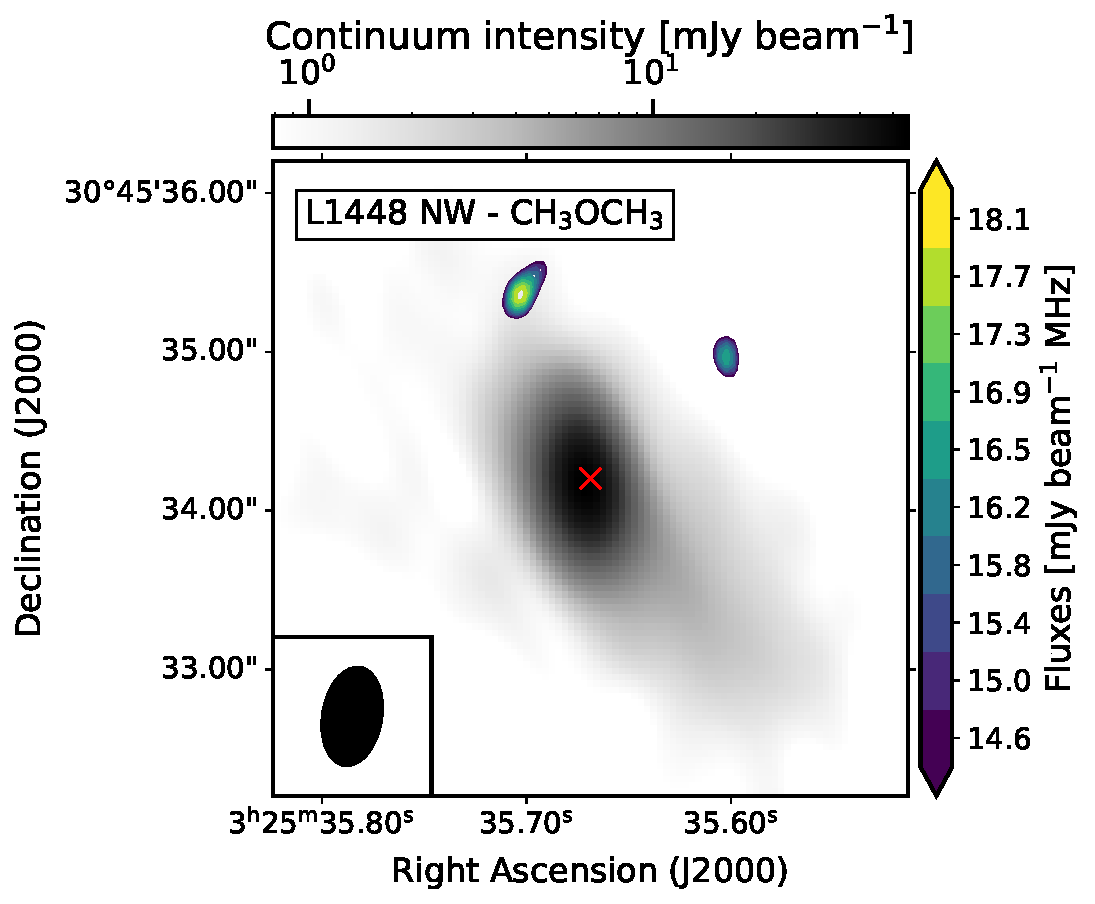
\includegraphics[width=0.24\textwidth]{/Users/yaolun/1d_spectra/extractions/moment0/subset/Set1_ID00_CH3OCH3_259311.pdf}
  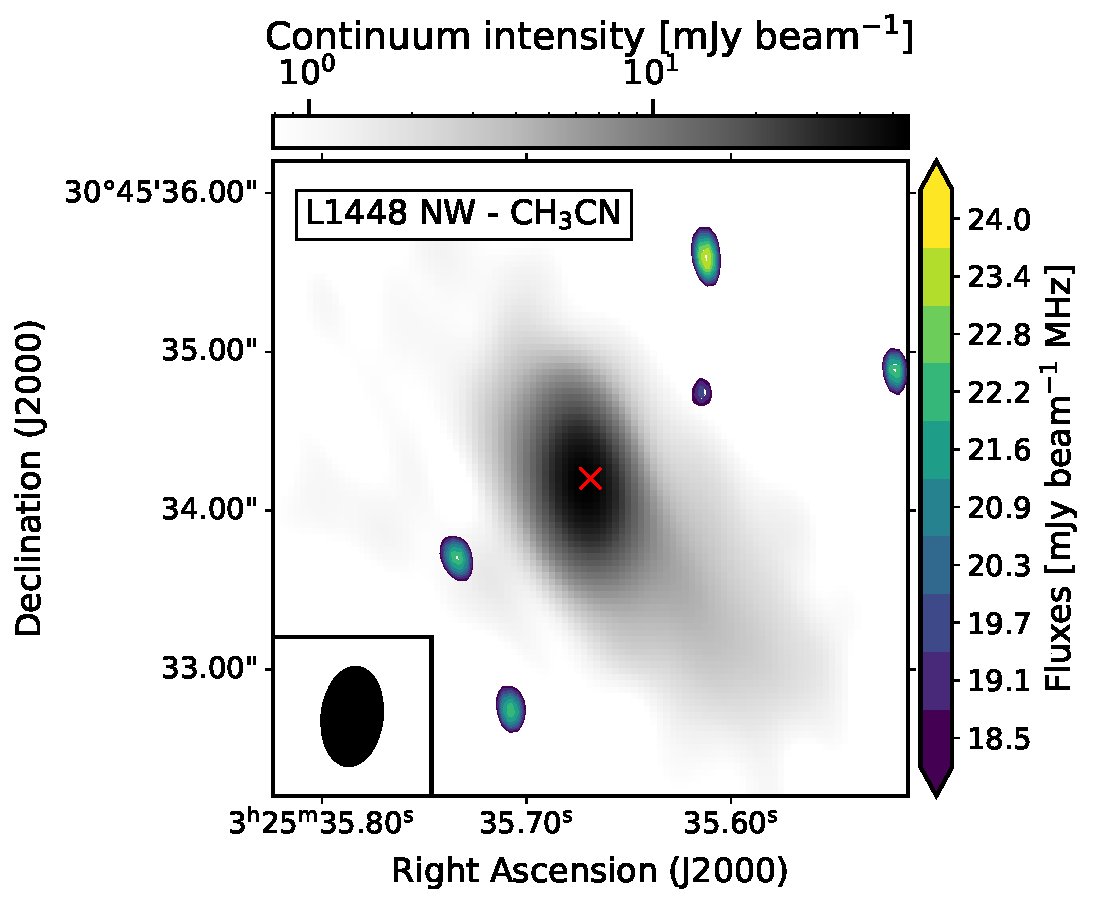
\includegraphics[width=0.24\textwidth]{/Users/yaolun/1d_spectra/extractions/moment0/subset/Set1_ID00_CH3CN_257527.pdf}
  \\
  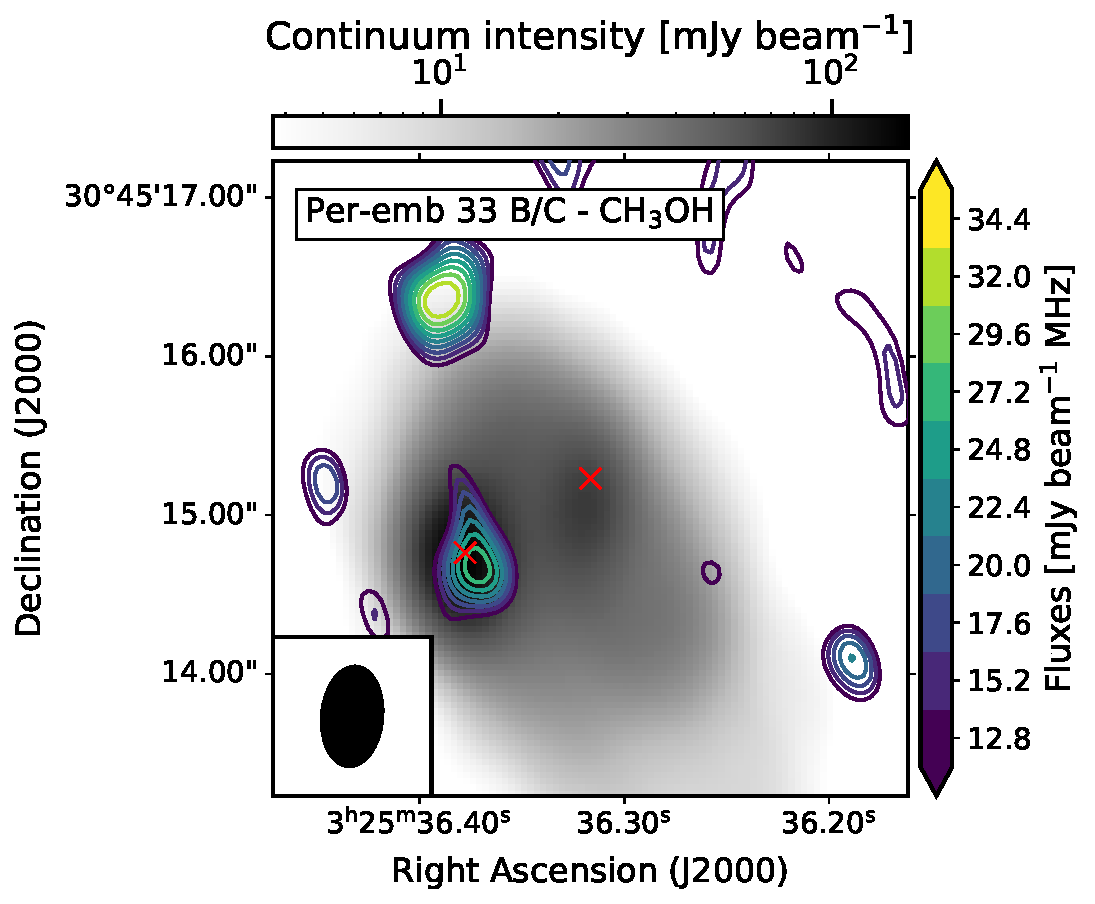
\includegraphics[width=0.24\textwidth]{/Users/yaolun/1d_spectra/extractions/moment0/subset/Set1_ID01_4_CH3OH_243915.pdf}
  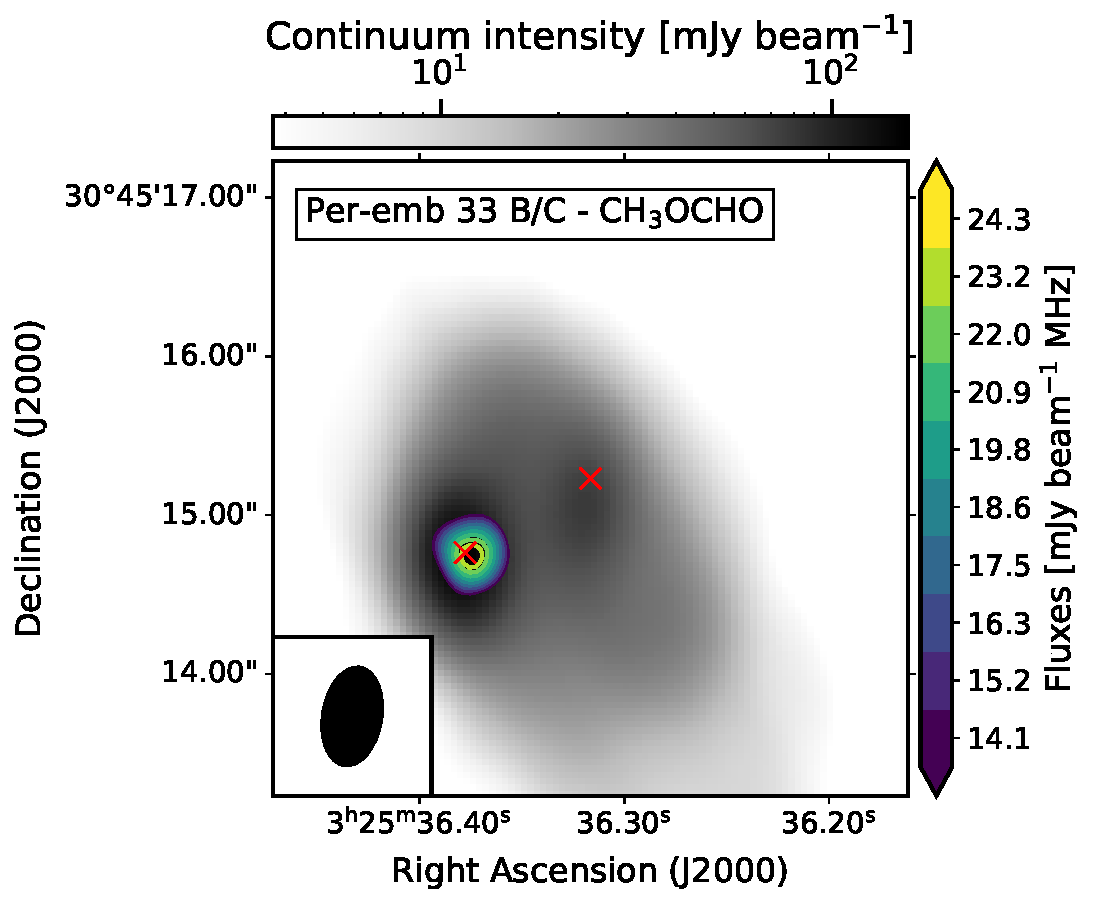
\includegraphics[width=0.24\textwidth]{/Users/yaolun/1d_spectra/extractions/moment0/subset/Set1_ID01_4_CH3OCHO_259342.pdf}
  \includegraphics[width=0.24\textwidth]{/Users/yaolun/1d_spectra/extractions/moment0/subset/Set1_ID01_4_CH3OCH3_259311.pdf}
  \includegraphics[width=0.24\textwidth]{/Users/yaolun/1d_spectra/extractions/moment0/subset/Set1_ID01_4_CH3CN_257527.pdf}
  \\
  \includegraphics[width=0.24\textwidth]{/Users/yaolun/1d_spectra/extractions/moment0/subset/Set1_ID01_CH3OH_243915.pdf}
  \includegraphics[width=0.24\textwidth]{/Users/yaolun/1d_spectra/extractions/moment0/subset/Set1_ID01_CH3OCHO_259342.pdf}
  \includegraphics[width=0.24\textwidth]{/Users/yaolun/1d_spectra/extractions/moment0/subset/Set1_ID01_CH3OCH3_259311.pdf}
  \includegraphics[width=0.24\textwidth]{/Users/yaolun/1d_spectra/extractions/moment0/subset/Set1_ID01_CH3CN_257527.pdf}
  \\
  \caption{The intensity maps of most detected COMs, \methanol, \methylcyanide, \methylformate, and \dimethylether\ (from left to right).  
          Each row shows the emission of a PEACHES protostar with increasing R.A.
          The intensity is calculated by integrating over 3\kms\ around the line centroid, while the lowest contour shows the 3$\sigma$ value.  
          The grayscale images illustrate the continuum emission.}
  \label{fig:coms_map_all}
\end{figure*}
\renewcommand{\thefigure}{\arabic{figure} (Cont.)}
\addtocounter{figure}{-1}
\begin{figure*}[htbp!]
  \centering
  \includegraphics[width=0.24\textwidth]{/Users/yaolun/1d_spectra/extractions/moment0/subset/Set1_ID01_3_CH3OH_243915.pdf}
  \includegraphics[width=0.24\textwidth]{/Users/yaolun/1d_spectra/extractions/moment0/subset/Set1_ID01_3_CH3OCHO_259342.pdf}
  \includegraphics[width=0.24\textwidth]{/Users/yaolun/1d_spectra/extractions/moment0/subset/Set1_ID01_3_CH3OCH3_259311.pdf}
  \includegraphics[width=0.24\textwidth]{/Users/yaolun/1d_spectra/extractions/moment0/subset/Set1_ID01_3_CH3CN_257527.pdf}
  \\
  \includegraphics[width=0.24\textwidth]{/Users/yaolun/1d_spectra/extractions/moment0/subset/Set1_ID01_2_CH3OH_243915.pdf}
  \includegraphics[width=0.24\textwidth]{/Users/yaolun/1d_spectra/extractions/moment0/subset/Set1_ID01_2_CH3OCHO_259342.pdf}
  \includegraphics[width=0.24\textwidth]{/Users/yaolun/1d_spectra/extractions/moment0/subset/Set1_ID01_2_CH3OCH3_259311.pdf}
  \includegraphics[width=0.24\textwidth]{/Users/yaolun/1d_spectra/extractions/moment0/subset/Set1_ID01_2_CH3CN_257527.pdf}
  \\
  \includegraphics[width=0.24\textwidth]{/Users/yaolun/1d_spectra/extractions/moment0/subset/Set1_ID02_CH3OH_243915.pdf}
  \includegraphics[width=0.24\textwidth]{/Users/yaolun/1d_spectra/extractions/moment0/subset/Set1_ID02_CH3OCHO_259342.pdf}
  \includegraphics[width=0.24\textwidth]{/Users/yaolun/1d_spectra/extractions/moment0/subset/Set1_ID02_CH3OCH3_259311.pdf}
  \includegraphics[width=0.24\textwidth]{/Users/yaolun/1d_spectra/extractions/moment0/subset/Set1_ID02_CH3CN_257527.pdf}
  \\
  \includegraphics[width=0.24\textwidth]{/Users/yaolun/1d_spectra/extractions/moment0/subset/Set1_ID02_2_CH3OH_243915.pdf}
  \includegraphics[width=0.24\textwidth]{/Users/yaolun/1d_spectra/extractions/moment0/subset/Set1_ID02_2_CH3OCHO_259342.pdf}
  \includegraphics[width=0.24\textwidth]{/Users/yaolun/1d_spectra/extractions/moment0/subset/Set1_ID02_2_CH3OCH3_259311.pdf}
  \includegraphics[width=0.24\textwidth]{/Users/yaolun/1d_spectra/extractions/moment0/subset/Set1_ID02_2_CH3CN_257527.pdf}
  \\
  \includegraphics[width=0.24\textwidth]{/Users/yaolun/1d_spectra/extractions/moment0/subset/Set1_ID05_CH3OH_243915.pdf}
  \includegraphics[width=0.24\textwidth]{/Users/yaolun/1d_spectra/extractions/moment0/subset/Set1_ID05_CH3OCHO_259342.pdf}
  \includegraphics[width=0.24\textwidth]{/Users/yaolun/1d_spectra/extractions/moment0/subset/Set1_ID05_CH3OCH3_259311.pdf}
  \includegraphics[width=0.24\textwidth]{/Users/yaolun/1d_spectra/extractions/moment0/subset/Set1_ID05_CH3CN_257527.pdf}
  \\
  \caption{}
\end{figure*}
\addtocounter{figure}{-1}
\begin{figure*}[htbp!]
  \centering
  \includegraphics[width=0.24\textwidth]{/Users/yaolun/1d_spectra/extractions/moment0/subset/Set1_ID06_CH3OH_243915.pdf}
  \includegraphics[width=0.24\textwidth]{/Users/yaolun/1d_spectra/extractions/moment0/subset/Set1_ID06_CH3OCHO_259342.pdf}
  \includegraphics[width=0.24\textwidth]{/Users/yaolun/1d_spectra/extractions/moment0/subset/Set1_ID06_CH3OCH3_259311.pdf}
  \includegraphics[width=0.24\textwidth]{/Users/yaolun/1d_spectra/extractions/moment0/subset/Set1_ID06_CH3CN_257527.pdf}
  \\
  \includegraphics[width=0.24\textwidth]{/Users/yaolun/1d_spectra/extractions/moment0/subset/Set1_ID07_CH3OH_243915.pdf}
  \includegraphics[width=0.24\textwidth]{/Users/yaolun/1d_spectra/extractions/moment0/subset/Set1_ID07_CH3OCHO_259342.pdf}
  \includegraphics[width=0.24\textwidth]{/Users/yaolun/1d_spectra/extractions/moment0/subset/Set1_ID07_CH3OCH3_259311.pdf}
  \includegraphics[width=0.24\textwidth]{/Users/yaolun/1d_spectra/extractions/moment0/subset/Set1_ID07_CH3CN_257527.pdf}
  \\
  \includegraphics[width=0.24\textwidth]{/Users/yaolun/1d_spectra/extractions/moment0/subset/Set1_ID08_CH3OH_243915.pdf}
  \includegraphics[width=0.24\textwidth]{/Users/yaolun/1d_spectra/extractions/moment0/subset/Set1_ID08_CH3OCHO_259342.pdf}
  \includegraphics[width=0.24\textwidth]{/Users/yaolun/1d_spectra/extractions/moment0/subset/Set1_ID08_CH3OCH3_259311.pdf}
  \includegraphics[width=0.24\textwidth]{/Users/yaolun/1d_spectra/extractions/moment0/subset/Set1_ID08_CH3CN_257527.pdf}
  \\
  \includegraphics[width=0.24\textwidth]{/Users/yaolun/1d_spectra/extractions/moment0/subset/Set2_ID07_CH3OH_243915.pdf}
  \includegraphics[width=0.24\textwidth]{/Users/yaolun/1d_spectra/extractions/moment0/subset/Set2_ID07_CH3OCHO_259342.pdf}
  \includegraphics[width=0.24\textwidth]{/Users/yaolun/1d_spectra/extractions/moment0/subset/Set2_ID07_CH3OCH3_259311.pdf}
  \includegraphics[width=0.24\textwidth]{/Users/yaolun/1d_spectra/extractions/moment0/subset/Set2_ID07_CH3CN_257527.pdf}
  \\
  \includegraphics[width=0.24\textwidth]{/Users/yaolun/1d_spectra/extractions/moment0/subset/Set2_ID07_2_CH3OH_243915.pdf}
  \includegraphics[width=0.24\textwidth]{/Users/yaolun/1d_spectra/extractions/moment0/subset/Set2_ID07_2_CH3OCHO_259342.pdf}
  \includegraphics[width=0.24\textwidth]{/Users/yaolun/1d_spectra/extractions/moment0/subset/Set2_ID07_2_CH3OCH3_259311.pdf}
  \includegraphics[width=0.24\textwidth]{/Users/yaolun/1d_spectra/extractions/moment0/subset/Set2_ID07_2_CH3CN_257527.pdf}
  \\
  \caption{}
\end{figure*}
\addtocounter{figure}{-1}
\begin{figure*}[htbp!]
  \centering
  \includegraphics[width=0.24\textwidth]{/Users/yaolun/1d_spectra/extractions/moment0/subset/Set2_ID03_CH3OH_243915.pdf}
  \includegraphics[width=0.24\textwidth]{/Users/yaolun/1d_spectra/extractions/moment0/subset/Set2_ID03_CH3OCHO_259342.pdf}
  \includegraphics[width=0.24\textwidth]{/Users/yaolun/1d_spectra/extractions/moment0/subset/Set2_ID03_CH3OCH3_259311.pdf}
  \includegraphics[width=0.24\textwidth]{/Users/yaolun/1d_spectra/extractions/moment0/subset/Set2_ID03_CH3CN_257527.pdf}
  \\
  \includegraphics[width=0.24\textwidth]{/Users/yaolun/1d_spectra/extractions/moment0/subset/Set2_ID16_CH3OH_243915.pdf}
  \includegraphics[width=0.24\textwidth]{/Users/yaolun/1d_spectra/extractions/moment0/subset/Set2_ID16_CH3OCHO_259342.pdf}
  \includegraphics[width=0.24\textwidth]{/Users/yaolun/1d_spectra/extractions/moment0/subset/Set2_ID16_CH3OCH3_259311.pdf}
  \includegraphics[width=0.24\textwidth]{/Users/yaolun/1d_spectra/extractions/moment0/subset/Set2_ID16_CH3CN_257527.pdf}
  \\
  \includegraphics[width=0.24\textwidth]{/Users/yaolun/1d_spectra/extractions/moment0/subset/Set2_ID04_CH3OH_243915.pdf}
  \includegraphics[width=0.24\textwidth]{/Users/yaolun/1d_spectra/extractions/moment0/subset/Set2_ID04_CH3OCHO_259342.pdf}
  \includegraphics[width=0.24\textwidth]{/Users/yaolun/1d_spectra/extractions/moment0/subset/Set2_ID04_CH3OCH3_259311.pdf}
  \includegraphics[width=0.24\textwidth]{/Users/yaolun/1d_spectra/extractions/moment0/subset/Set2_ID04_CH3CN_257527.pdf}
  \\
  \includegraphics[width=0.24\textwidth]{/Users/yaolun/1d_spectra/extractions/moment0/subset/Set2_ID08_CH3OH_243915.pdf}
  \includegraphics[width=0.24\textwidth]{/Users/yaolun/1d_spectra/extractions/moment0/subset/Set2_ID08_CH3OCHO_259342.pdf}
  \includegraphics[width=0.24\textwidth]{/Users/yaolun/1d_spectra/extractions/moment0/subset/Set2_ID08_CH3OCH3_259311.pdf}
  \includegraphics[width=0.24\textwidth]{/Users/yaolun/1d_spectra/extractions/moment0/subset/Set2_ID08_CH3CN_257527.pdf}
  \\
  \includegraphics[width=0.24\textwidth]{/Users/yaolun/1d_spectra/extractions/moment0/subset/Set2_ID00_2_CH3OH_243915.pdf}
  \includegraphics[width=0.24\textwidth]{/Users/yaolun/1d_spectra/extractions/moment0/subset/Set2_ID00_2_CH3OCHO_259342.pdf}
  \includegraphics[width=0.24\textwidth]{/Users/yaolun/1d_spectra/extractions/moment0/subset/Set2_ID00_2_CH3OCH3_259311.pdf}
  \includegraphics[width=0.24\textwidth]{/Users/yaolun/1d_spectra/extractions/moment0/subset/Set2_ID00_2_CH3CN_257527.pdf}
  \\
  \caption{}
\end{figure*}
\addtocounter{figure}{-1}
\begin{figure*}[htbp!]
  \centering
  \includegraphics[width=0.24\textwidth]{/Users/yaolun/1d_spectra/extractions/moment0/subset/Set2_ID00_CH3OH_243915.pdf}
  \includegraphics[width=0.24\textwidth]{/Users/yaolun/1d_spectra/extractions/moment0/subset/Set2_ID00_CH3OCHO_259342.pdf}
  \includegraphics[width=0.24\textwidth]{/Users/yaolun/1d_spectra/extractions/moment0/subset/Set2_ID00_CH3OCH3_259311.pdf}
  \includegraphics[width=0.24\textwidth]{/Users/yaolun/1d_spectra/extractions/moment0/subset/Set2_ID00_CH3CN_257527.pdf}
  \\
  \includegraphics[width=0.24\textwidth]{/Users/yaolun/1d_spectra/extractions/moment0/subset/Set2_ID09_CH3OH_243915.pdf}
  \includegraphics[width=0.24\textwidth]{/Users/yaolun/1d_spectra/extractions/moment0/subset/Set2_ID09_CH3OCHO_259342.pdf}
  \includegraphics[width=0.24\textwidth]{/Users/yaolun/1d_spectra/extractions/moment0/subset/Set2_ID09_CH3OCH3_259311.pdf}
  \includegraphics[width=0.24\textwidth]{/Users/yaolun/1d_spectra/extractions/moment0/subset/Set2_ID09_CH3CN_257527.pdf}
  \\
  \includegraphics[width=0.24\textwidth]{/Users/yaolun/1d_spectra/extractions/moment0/subset/Set2_ID11_CH3OH_243915.pdf}
  \includegraphics[width=0.24\textwidth]{/Users/yaolun/1d_spectra/extractions/moment0/subset/Set2_ID11_CH3OCHO_259342.pdf}
  \includegraphics[width=0.24\textwidth]{/Users/yaolun/1d_spectra/extractions/moment0/subset/Set2_ID11_CH3OCH3_259311.pdf}
  \includegraphics[width=0.24\textwidth]{/Users/yaolun/1d_spectra/extractions/moment0/subset/Set2_ID11_CH3CN_257527.pdf}
  \\
  \includegraphics[width=0.24\textwidth]{/Users/yaolun/1d_spectra/extractions/moment0/subset/Set2_ID01_2_CH3OH_243915.pdf}
  \includegraphics[width=0.24\textwidth]{/Users/yaolun/1d_spectra/extractions/moment0/subset/Set2_ID01_2_CH3OCHO_259342.pdf}
  \includegraphics[width=0.24\textwidth]{/Users/yaolun/1d_spectra/extractions/moment0/subset/Set2_ID01_2_CH3OCH3_259311.pdf}
  \includegraphics[width=0.24\textwidth]{/Users/yaolun/1d_spectra/extractions/moment0/subset/Set2_ID01_2_CH3CN_257527.pdf}
  \\
  \includegraphics[width=0.24\textwidth]{/Users/yaolun/1d_spectra/extractions/moment0/subset/Set2_ID01_CH3OH_243915.pdf}
  \includegraphics[width=0.24\textwidth]{/Users/yaolun/1d_spectra/extractions/moment0/subset/Set2_ID01_CH3OCHO_259342.pdf}
  \includegraphics[width=0.24\textwidth]{/Users/yaolun/1d_spectra/extractions/moment0/subset/Set2_ID01_CH3OCH3_259311.pdf}
  \includegraphics[width=0.24\textwidth]{/Users/yaolun/1d_spectra/extractions/moment0/subset/Set2_ID01_CH3CN_257527.pdf}
  \\
  \caption{}
\end{figure*}
\addtocounter{figure}{-1}
\begin{figure*}[htbp!]
  \centering
  \includegraphics[width=0.24\textwidth]{/Users/yaolun/1d_spectra/extractions/moment0/subset/Set2_ID05_CH3OH_243915.pdf}
  \includegraphics[width=0.24\textwidth]{/Users/yaolun/1d_spectra/extractions/moment0/subset/Set2_ID05_CH3OCHO_259342.pdf}
  \includegraphics[width=0.24\textwidth]{/Users/yaolun/1d_spectra/extractions/moment0/subset/Set2_ID05_CH3OCH3_259311.pdf}
  \includegraphics[width=0.24\textwidth]{/Users/yaolun/1d_spectra/extractions/moment0/subset/Set2_ID05_CH3CN_257527.pdf}
  \\
  \includegraphics[width=0.24\textwidth]{/Users/yaolun/1d_spectra/extractions/moment0/subset/Set2_ID12_CH3OH_243915.pdf}
  \includegraphics[width=0.24\textwidth]{/Users/yaolun/1d_spectra/extractions/moment0/subset/Set2_ID12_CH3OCHO_259342.pdf}
  \includegraphics[width=0.24\textwidth]{/Users/yaolun/1d_spectra/extractions/moment0/subset/Set2_ID12_CH3OCH3_259311.pdf}
  \includegraphics[width=0.24\textwidth]{/Users/yaolun/1d_spectra/extractions/moment0/subset/Set2_ID12_CH3CN_257527.pdf}
  \\
  \includegraphics[width=0.24\textwidth]{/Users/yaolun/1d_spectra/extractions/moment0/subset/Set2_ID02_CH3OH_243915.pdf}
  \includegraphics[width=0.24\textwidth]{/Users/yaolun/1d_spectra/extractions/moment0/subset/Set2_ID02_CH3OCHO_259342.pdf}
  \includegraphics[width=0.24\textwidth]{/Users/yaolun/1d_spectra/extractions/moment0/subset/Set2_ID02_CH3OCH3_259311.pdf}
  \includegraphics[width=0.24\textwidth]{/Users/yaolun/1d_spectra/extractions/moment0/subset/Set2_ID02_CH3CN_257527.pdf}
  \\
  \includegraphics[width=0.24\textwidth]{/Users/yaolun/1d_spectra/extractions/moment0/subset/Set2_ID02_2_CH3OH_243915.pdf}
  \includegraphics[width=0.24\textwidth]{/Users/yaolun/1d_spectra/extractions/moment0/subset/Set2_ID02_2_CH3OCHO_259342.pdf}
  \includegraphics[width=0.24\textwidth]{/Users/yaolun/1d_spectra/extractions/moment0/subset/Set2_ID02_2_CH3OCH3_259311.pdf}
  \includegraphics[width=0.24\textwidth]{/Users/yaolun/1d_spectra/extractions/moment0/subset/Set2_ID02_2_CH3CN_257527.pdf}
  \\
  \includegraphics[width=0.24\textwidth]{/Users/yaolun/1d_spectra/extractions/moment0/subset/Set2_ID06_CH3OH_243915.pdf}
  \includegraphics[width=0.24\textwidth]{/Users/yaolun/1d_spectra/extractions/moment0/subset/Set2_ID06_CH3OCHO_259342.pdf}
  \includegraphics[width=0.24\textwidth]{/Users/yaolun/1d_spectra/extractions/moment0/subset/Set2_ID06_CH3OCH3_259311.pdf}
  \includegraphics[width=0.24\textwidth]{/Users/yaolun/1d_spectra/extractions/moment0/subset/Set2_ID06_CH3CN_257527.pdf}
  \\
  \caption{}
\end{figure*}
\addtocounter{figure}{-1}
\begin{figure*}[htbp!]
  \centering
  \includegraphics[width=0.24\textwidth]{/Users/yaolun/1d_spectra/extractions/moment0/subset/Set2_ID13_2_CH3OH_243915.pdf}
  \includegraphics[width=0.24\textwidth]{/Users/yaolun/1d_spectra/extractions/moment0/subset/Set2_ID13_2_CH3OCHO_259342.pdf}
  \includegraphics[width=0.24\textwidth]{/Users/yaolun/1d_spectra/extractions/moment0/subset/Set2_ID13_2_CH3OCH3_259311.pdf}
  \includegraphics[width=0.24\textwidth]{/Users/yaolun/1d_spectra/extractions/moment0/subset/Set2_ID13_2_CH3CN_257527.pdf}
  \\
  \includegraphics[width=0.24\textwidth]{/Users/yaolun/1d_spectra/extractions/moment0/subset/Set2_ID13_CH3OH_243915.pdf}
  \includegraphics[width=0.24\textwidth]{/Users/yaolun/1d_spectra/extractions/moment0/subset/Set2_ID13_CH3OCHO_259342.pdf}
  \includegraphics[width=0.24\textwidth]{/Users/yaolun/1d_spectra/extractions/moment0/subset/Set2_ID13_CH3OCH3_259311.pdf}
  \includegraphics[width=0.24\textwidth]{/Users/yaolun/1d_spectra/extractions/moment0/subset/Set2_ID13_CH3CN_257527.pdf}
  \\
  \includegraphics[width=0.24\textwidth]{/Users/yaolun/1d_spectra/extractions/moment0/subset/Set3_ID05_CH3OH_243915.pdf}
  \includegraphics[width=0.24\textwidth]{/Users/yaolun/1d_spectra/extractions/moment0/subset/Set3_ID05_CH3OCHO_259342.pdf}
  \includegraphics[width=0.24\textwidth]{/Users/yaolun/1d_spectra/extractions/moment0/subset/Set3_ID05_CH3OCH3_259311.pdf}
  \includegraphics[width=0.24\textwidth]{/Users/yaolun/1d_spectra/extractions/moment0/subset/Set3_ID05_CH3CN_257527.pdf}
  \\
  \includegraphics[width=0.24\textwidth]{/Users/yaolun/1d_spectra/extractions/moment0/subset/Set3_ID04_CH3OH_243915.pdf}
  \includegraphics[width=0.24\textwidth]{/Users/yaolun/1d_spectra/extractions/moment0/subset/Set3_ID04_CH3OCHO_259342.pdf}
  \includegraphics[width=0.24\textwidth]{/Users/yaolun/1d_spectra/extractions/moment0/subset/Set3_ID04_CH3OCH3_259311.pdf}
  \includegraphics[width=0.24\textwidth]{/Users/yaolun/1d_spectra/extractions/moment0/subset/Set3_ID04_CH3CN_257527.pdf}
  \\
  \includegraphics[width=0.24\textwidth]{/Users/yaolun/1d_spectra/extractions/moment0/subset/Set3_ID02_CH3OH_243915.pdf}
  \includegraphics[width=0.24\textwidth]{/Users/yaolun/1d_spectra/extractions/moment0/subset/Set3_ID02_CH3OCHO_259342.pdf}
  \includegraphics[width=0.24\textwidth]{/Users/yaolun/1d_spectra/extractions/moment0/subset/Set3_ID02_CH3OCH3_259311.pdf}
  \includegraphics[width=0.24\textwidth]{/Users/yaolun/1d_spectra/extractions/moment0/subset/Set3_ID02_CH3CN_257527.pdf}
  \\
  \caption{}
\end{figure*}
\addtocounter{figure}{-1}
\begin{figure*}[htbp!]
  \centering
  \includegraphics[width=0.24\textwidth]{/Users/yaolun/1d_spectra/extractions/moment0/subset/Set3_ID03_CH3OH_243915.pdf}
  \includegraphics[width=0.24\textwidth]{/Users/yaolun/1d_spectra/extractions/moment0/subset/Set3_ID03_CH3OCHO_259342.pdf}
  \includegraphics[width=0.24\textwidth]{/Users/yaolun/1d_spectra/extractions/moment0/subset/Set3_ID03_CH3OCH3_259311.pdf}
  \includegraphics[width=0.24\textwidth]{/Users/yaolun/1d_spectra/extractions/moment0/subset/Set3_ID03_CH3CN_257527.pdf}
  \\
  \includegraphics[width=0.24\textwidth]{/Users/yaolun/1d_spectra/extractions/moment0/subset/Set3_ID01_CH3OH_243915.pdf}
  \includegraphics[width=0.24\textwidth]{/Users/yaolun/1d_spectra/extractions/moment0/subset/Set3_ID01_CH3OCHO_259342.pdf}
  \includegraphics[width=0.24\textwidth]{/Users/yaolun/1d_spectra/extractions/moment0/subset/Set3_ID01_CH3OCH3_259311.pdf}
  \includegraphics[width=0.24\textwidth]{/Users/yaolun/1d_spectra/extractions/moment0/subset/Set3_ID01_CH3CN_257527.pdf}
  \\
  \includegraphics[width=0.24\textwidth]{/Users/yaolun/1d_spectra/extractions/moment0/subset/Set3_ID00_2_CH3OH_243915.pdf}
  \includegraphics[width=0.24\textwidth]{/Users/yaolun/1d_spectra/extractions/moment0/subset/Set3_ID00_2_CH3OCHO_259342.pdf}
  \includegraphics[width=0.24\textwidth]{/Users/yaolun/1d_spectra/extractions/moment0/subset/Set3_ID00_2_CH3OCH3_259311.pdf}
  \includegraphics[width=0.24\textwidth]{/Users/yaolun/1d_spectra/extractions/moment0/subset/Set3_ID00_2_CH3CN_257527.pdf}
  \\
  \includegraphics[width=0.24\textwidth]{/Users/yaolun/1d_spectra/extractions/moment0/subset/Set3_ID00_CH3OH_243915.pdf}
  \includegraphics[width=0.24\textwidth]{/Users/yaolun/1d_spectra/extractions/moment0/subset/Set3_ID00_CH3OCHO_259342.pdf}
  \includegraphics[width=0.24\textwidth]{/Users/yaolun/1d_spectra/extractions/moment0/subset/Set3_ID00_CH3OCH3_259311.pdf}
  \includegraphics[width=0.24\textwidth]{/Users/yaolun/1d_spectra/extractions/moment0/subset/Set3_ID00_CH3CN_257527.pdf}
  \\
  \includegraphics[width=0.24\textwidth]{/Users/yaolun/1d_spectra/extractions/moment0/subset/Set3_ID09_CH3OH_243915.pdf}
  \includegraphics[width=0.24\textwidth]{/Users/yaolun/1d_spectra/extractions/moment0/subset/Set3_ID09_CH3OCHO_259342.pdf}
  \includegraphics[width=0.24\textwidth]{/Users/yaolun/1d_spectra/extractions/moment0/subset/Set3_ID09_CH3OCH3_259311.pdf}
  \includegraphics[width=0.24\textwidth]{/Users/yaolun/1d_spectra/extractions/moment0/subset/Set3_ID09_CH3CN_257527.pdf}
  \\
  \caption{}
\end{figure*}
\addtocounter{figure}{-1}
\begin{figure*}[htbp!]
  \centering
  \includegraphics[width=0.24\textwidth]{/Users/yaolun/1d_spectra/extractions/moment0/subset/Set3_ID09_2_CH3OH_243915.pdf}
  \includegraphics[width=0.24\textwidth]{/Users/yaolun/1d_spectra/extractions/moment0/subset/Set3_ID09_2_CH3OCHO_259342.pdf}
  \includegraphics[width=0.24\textwidth]{/Users/yaolun/1d_spectra/extractions/moment0/subset/Set3_ID09_2_CH3OCH3_259311.pdf}
  \includegraphics[width=0.24\textwidth]{/Users/yaolun/1d_spectra/extractions/moment0/subset/Set3_ID09_2_CH3CN_257527.pdf}
  \\
  \includegraphics[width=0.24\textwidth]{/Users/yaolun/1d_spectra/extractions/moment0/subset/Set3_ID06_CH3OH_243915.pdf}
  \includegraphics[width=0.24\textwidth]{/Users/yaolun/1d_spectra/extractions/moment0/subset/Set3_ID06_CH3OCHO_259342.pdf}
  \includegraphics[width=0.24\textwidth]{/Users/yaolun/1d_spectra/extractions/moment0/subset/Set3_ID06_CH3OCH3_259311.pdf}
  \includegraphics[width=0.24\textwidth]{/Users/yaolun/1d_spectra/extractions/moment0/subset/Set3_ID06_CH3CN_257527.pdf}
  \\
  \includegraphics[width=0.24\textwidth]{/Users/yaolun/1d_spectra/extractions/moment0/subset/Set3_ID07_2_CH3OH_243915.pdf}
  \includegraphics[width=0.24\textwidth]{/Users/yaolun/1d_spectra/extractions/moment0/subset/Set3_ID07_2_CH3OCHO_259342.pdf}
  \includegraphics[width=0.24\textwidth]{/Users/yaolun/1d_spectra/extractions/moment0/subset/Set3_ID07_2_CH3OCH3_259311.pdf}
  \includegraphics[width=0.24\textwidth]{/Users/yaolun/1d_spectra/extractions/moment0/subset/Set3_ID07_2_CH3CN_257527.pdf}
  \\
  \includegraphics[width=0.24\textwidth]{/Users/yaolun/1d_spectra/extractions/moment0/subset/Set3_ID07_CH3OH_243915.pdf}
  \includegraphics[width=0.24\textwidth]{/Users/yaolun/1d_spectra/extractions/moment0/subset/Set3_ID07_CH3OCHO_259342.pdf}
  \includegraphics[width=0.24\textwidth]{/Users/yaolun/1d_spectra/extractions/moment0/subset/Set3_ID07_CH3OCH3_259311.pdf}
  \includegraphics[width=0.24\textwidth]{/Users/yaolun/1d_spectra/extractions/moment0/subset/Set3_ID07_CH3CN_257527.pdf}
  \\
  \includegraphics[width=0.24\textwidth]{/Users/yaolun/1d_spectra/extractions/moment0/subset/Set3_ID07_3_CH3OH_243915.pdf}
  \includegraphics[width=0.24\textwidth]{/Users/yaolun/1d_spectra/extractions/moment0/subset/Set3_ID07_3_CH3OCHO_259342.pdf}
  \includegraphics[width=0.24\textwidth]{/Users/yaolun/1d_spectra/extractions/moment0/subset/Set3_ID07_3_CH3OCH3_259311.pdf}
  \includegraphics[width=0.24\textwidth]{/Users/yaolun/1d_spectra/extractions/moment0/subset/Set3_ID07_3_CH3CN_257527.pdf}
  \\
  \caption{}
\end{figure*}
\addtocounter{figure}{-1}
\begin{figure*}[htbp!]
  \centering
  \includegraphics[width=0.24\textwidth]{/Users/yaolun/1d_spectra/extractions/moment0/subset/Set3_ID08_2_CH3OH_243915.pdf}
  \includegraphics[width=0.24\textwidth]{/Users/yaolun/1d_spectra/extractions/moment0/subset/Set3_ID08_2_CH3OCHO_259342.pdf}
  \includegraphics[width=0.24\textwidth]{/Users/yaolun/1d_spectra/extractions/moment0/subset/Set3_ID08_2_CH3OCH3_259311.pdf}
  \includegraphics[width=0.24\textwidth]{/Users/yaolun/1d_spectra/extractions/moment0/subset/Set3_ID08_2_CH3CN_257527.pdf}
  \\
  \includegraphics[width=0.24\textwidth]{/Users/yaolun/1d_spectra/extractions/moment0/subset/Set3_ID08_CH3OH_243915.pdf}
  \includegraphics[width=0.24\textwidth]{/Users/yaolun/1d_spectra/extractions/moment0/subset/Set3_ID08_CH3OCHO_259342.pdf}
  \includegraphics[width=0.24\textwidth]{/Users/yaolun/1d_spectra/extractions/moment0/subset/Set3_ID08_CH3OCH3_259311.pdf}
  \includegraphics[width=0.24\textwidth]{/Users/yaolun/1d_spectra/extractions/moment0/subset/Set3_ID08_CH3CN_257527.pdf}
  \\
  \includegraphics[width=0.24\textwidth]{/Users/yaolun/1d_spectra/extractions/moment0/subset/Set3_ID10_CH3OH_243915.pdf}
  \includegraphics[width=0.24\textwidth]{/Users/yaolun/1d_spectra/extractions/moment0/subset/Set3_ID10_CH3OCHO_259342.pdf}
  \includegraphics[width=0.24\textwidth]{/Users/yaolun/1d_spectra/extractions/moment0/subset/Set3_ID10_CH3OCH3_259311.pdf}
  \includegraphics[width=0.24\textwidth]{/Users/yaolun/1d_spectra/extractions/moment0/subset/Set3_ID10_CH3CN_257527.pdf}
  \\
  \caption{}
\end{figure*}
\renewcommand{\thefigure}{\arabic{figure}}

\section{The Spectra of \cch}
The \cch\ spectra toward the continuum emission have irregular line profiles.  Some spectra have strong self-absorption, while some spectra only show the blue-shifted emission.  Due to the absorption and irregular line profile, the \textsc{xclass} fitting routine often fails to faithfully reproduce the observed \cch\ spectra.  \cch\ can easily form in the outflow cavity wall due to the abundant CH$_{4}$ sublimated from dust grains as well as C$^+$ ionized by the UV radiation.  Thus, the \cch\ spectra can have broad line width and multiple components.  Furthermore, the morphology of the \cch\ emission traces the outflows, making our extraction from the continuum emission non-ideal for representing the nature of the \cch\ emission.  \textcolor{red}{Figure\,\ref{fig:all_cch} and Y show the spectra and the moment 0 map of \cch, respectively.}

\begin{figure}[htbp!]
  \centering
  \includegraphics[width=0.47\textwidth]{Ncol_ch3oh_cch.pdf}
  \caption{Correlation of the column densities of \cch\ and \methanol\ fitted from the PEACHES protostars.  The sources where both molecules are detected are shown in black; the sources where only one molecule is detected are shown in magenta; finally, the sources where both molecules are not detected are shown in black for the corresponding upper limits.}
  \label{fig:cch_ch3oh}
\end{figure}

\begin{figure*}[htbp!]
  \centering
  \includegraphics[width=\textwidth]{all_cch.pdf}
  \caption{The \cch\ spectra of all PEACHES sources extracted from the continuum emission.}
  \label{fig:all_cch}
\end{figure*}

% \section{Notes on the COMs Modeling}
% \section{Notes on the 1D Spectra}
% \paragraph{L1448 IRS 3A}
% \begin{itemize}
%   \item The emission of SO and CS shows additional red-shifted component, separated by $\sim$4.6\kms.
% \end{itemize}

\paragraph{Per-emb-33-A}
\begin{itemize}
    \item The fitting of \methylformate\ reproduces the the strongest emission at 259343\mhz, but underestimates the emission between 246275\mhz\ to 247070\mhz, where the emission is at most 0.5\,K.  Considering the narrow absorption in HCN, CS, and SO lines as well as the brighter continuum temperature (10.5\,K), the emission of \methylformate\ may be affected by the continuum opacity.
%   \item Strong absorption at 246509\mhz.
%   \item HDCO seems to have two components for the transition at 246925\mhz, but the one at 259035\mhz\ only has one component, which is underestimated by the model.
\end{itemize}

% \paragraph{Per-emb-33-B/C}
% \begin{itemize}
%   \item CCH shows three components leading to an inaccurate fit.
% \end{itemize}

% \paragraph{Per-emb-42}
% \begin{itemize}
%   \item Double-peaked CS line
%   \item Triple-peaked CCH line
% \end{itemize}

\paragraph{Per-emb-26}
\begin{itemize}
  % \item Red-shifted excess appears in the CS, SO, \methanol, \htcn, and HDCO lines.
  \item Red-shifted excess appears in the \methanol\ lines.
  % \item Broad SO lines peak at slightly blue-shifted velocity ($\sim$1\kms).
  % \item The best-fitting model overestimates the \ethylcyanide, \acetaldehyde, and \cctht\ lines, possibly due to the contamination of SiO, which should have been excluded for fitting.  Tests are running now.
  % \item The secondary \methanol\ line becomes overestimated at $T_\text{ex} \geq $200 K.
  \item Unidentified lines at 246525\mhz\ and 244249\mhz.
\end{itemize}

% \paragraph{Per-emb-22-B}
% \begin{itemize}
%   \item The SO lines have small red-shifted excess.  The best-fitting line strength decreases significantly at $T_\text{ex} = $200 K.  Not sure why.
%   \item The SO line profiles are slightly skewed toward blue-shifted velocity, while the CS line shows another brighter peak at blue-shifted velocity.
% \end{itemize}

% \paragraph{Per-emb-22-A}
% \begin{itemize}
%   \item Hints of \methylformate emission, but not significant enough to warrant a detection.
% \end{itemize}

\paragraph{Per-emb-17}
\begin{itemize}
  \item Many line profiles exhibit a broad double-peaked profile, separated by $\sim$5--6\kms.  Per-emb-17 is a binary system unresolved by our observations.  However, the channel maps suggest that the two components are likely to surrounding the southern source, Per-emb-17-B.
  \item The \methylformate\ line at $\sim$259343\mhz\ may be optically thick.
\end{itemize}

% \paragraph{Per-emb-20}
% \begin{itemize}
%   \item The CCH lines have a narrow double-peaked profile.  The CS line shows a similar double-peak profile.
%   \item The SO lines have a broad component underneath the typical narrow lines.
% \end{itemize}

\paragraph{SVS13 A2}
\begin{itemize}
  \item Weak indication of the unidentified line at 246525\mhz, which has been detected in other sources.
  % \item The model strength of CCH suddenly decreases at $T_\text{ex} = $200 K by $\sim$0.5 K over a 2 K line.
\end{itemize}

\paragraph{Per-emb-44}
\begin{itemize}
  \item Unidentified lines at 244248\mhz, 246219\mhz, 246254\mhz, 246344\mhz, 246389\mhz, 246434\mhz, 246525\mhz, 246838\mhz, 258268\mhz, 258271\mhz, and 262068-262070\mhz.
  \item Higher temperatures ($T\text{ex} > $100 K) provide better fittings.  Probably should adopt the temperature fitted from \methylformate\ (previous MCMC fitting suggests a temperature of 263 K).
\end{itemize}

\paragraph{Per-emb-12-B}
\begin{itemize}
  \item Unidentified lines at 244248\mhz, 246254\mhz, 246314\mhz, 246322\mhz, 246389\mhz, 246434\mhz, 246525\mhz, 246696\mhz, 246838\mhz, 246873\mhz, 247082\mhz, 258268\mhz, 258271\mhz, and 262068-262070\mhz.
\end{itemize}

\paragraph{Per-emb-12-A}
\begin{itemize}
  \item Strong absorption features detected across the spectra, CCH, SO, \htcn, CS, \methanol, HDCO, \methylcyanide, and \methylformate.
\end{itemize}

\paragraph{IRAS4B$\prime$}
\begin{itemize}
  \item Spectra show no emission along with absorption at SO, CS, and \methanol\ lines.
\end{itemize}

\paragraph{Per-emb-13}
\begin{itemize}
  \item The \methylformate\ emission needs $T_\text{ex} > $100 K to have a good fit.
  \item All three \methanol\ lines are detected but two of them show clear sign of self-absorption, therefore, not ideal for fitting the excitation temperature.
  \item Unidentified lines at 244248\mhz, 246254\mhz, 246331\mhz, 246344\mhz, 246434\mhz, 246525\mhz, 246838\mhz, 246974\mhz, 247086\mhz, 257268\mhz, 257271\mhz, 259323\mhz, 259331\mhz, 262098\mhz, and 262109\mhz.
  % \item The best-fitting models have two different widths for the \acetaldehyde\ lines.  
  \item The best-fitting model for \tmethanol\ lines overestimates the line width due to the weak and broad line at 247086\mhz.
\end{itemize}

\paragraph{Per-emb-27}
\begin{itemize}
  \item All three \methanol\ lines are detected, but none of the temperature produce a good fit to all three lines, suggesting that some lines are optically thick.  The intensities of the transitions at 243916\mhz\ and 261806\mhz\ are $\sim$30 K, while the intensity at 246873\mhz\ is about 24 K.  They seems to be optically thick.  In comparison, the continuum brightness temperature is only 5.8 K.
  \item Unidentified lines at 244232\mhz, 244248\mhz, 246207\mhz, 246254\mhz, 246388\mhz, 246435\mhz, 246525\mhz, 246538\mhz, 246838\mhz, 246973\mhz, 247084\mhz, and 259330\mhz.
  \item The \methanol\ line at 243916\mhz\ and the SO lines become optically thick at 100 K.
\end{itemize}

% \paragraph{Per-emb-54}
% \begin{itemize}
%   \item The SO lines appears red-shifted by $\sim$2\kms.
%   \item The emission of CS and CCH shows a blue-shifted peak along with absorption slightly red-shifted compared to the source velocity.
% \end{itemize}

\paragraph{Per-emb-21}
\begin{itemize}
  \item Emission of \methanol\ is detected.  However, the broad width and noisy spectra lead to a bad fit.  The best-fitting model has the maximum line width allowed, 3.5\kms.
\end{itemize}

% \paragraph{Per-emb-14}
% \begin{itemize}
%   \item The best-fitting model underestimates the HDCO lines, possibly due to the simultaneously fitted \tmethanol\ lines.
% \end{itemize}

\paragraph{Per-emb-35-B}
\begin{itemize}
  % \item The best-fitting model underestimates the SO lines at $T_\text{ex} = $100 K.
  % \item The CCH lines show a double-peaked line profile.
  \item The \methanol\ line at 243915\mhz has an S/N of 1.2, but hints the existence of \methanol.
\end{itemize}

\paragraph{Per-emb-35-A}
\begin{itemize}
  \item The goodness of fitting for the \methanol\ lines is a strong function of temperature, suggesting that the \methanol\ lines can indicate the $T_\text{ex}$.
  \item The \methylformate\ line at 259342\mhz\ has an S/N of 1.8, but hint the existence of \methylformate.
\end{itemize}

% \paragraph{SVS13B}
% \begin{itemize}
%   \item The fitted width of the HDCO lines is overestimated.
% \end{itemize}

\paragraph{Per-emb-15}
\begin{itemize}
  \item All lines have only the blue-shifted emission, making them blue-asymmetric.
\end{itemize}

% \paragraph{Per-emb-50}
% \begin{itemize}
%   \item The SO and SO$_{2}$ lines have a very broad component ($\Delta \nu = $6\kms), skewing toward the blue-shifted velocity.
% \end{itemize}

\paragraph{Per-emb-18}
\begin{itemize}
  \item Many transitions of \methylformate\ are tentatively detected; however, none of them has S/N $>$ 3.  Currently categorized as non-detection.
  % \item The HDCO lines are broader than the maximum allowed line width, 3.5\kms, making the fitting inaccurate.
\end{itemize}

% \paragraph{Per-emb-37}
% \begin{itemize}
%   \item The fitting of SO lines has a strong variation as a function of temperatures.
% \end{itemize}

% \paragraph{Per-emb-36}
% \begin{itemize}
%   \item The SO lines are underestimated by the best-fitting model.  Perhaps it can be fixed by changing the \texttt{Variation} parameter.  To be tested.  Test run on laptop shows no issue of having a good fit at 100 K for SO with \texttt{Variation} $= 10^{-2}$.
%   \item The CCH lines only show at the blue-shifted velocities.
% \end{itemize}

\paragraph{B1-bS}
\begin{itemize}
  \item Higher temperatures produce worse fittings to the \methylformate\ lines.  Previous MCMC fitting of the \methylformate\ lines suggests a temperature of 58 K.
  \item The fitting of \dimethylether\ is limited by the minimum line width of 1.2\kms.  
  \item Unidentified lines at 246027\mhz, 246099\mhz, 246143\mhz, 246192\mhz, 246525\mhz, 246674\mhz, and 2467320\mhz.
  \item The \methylformate\ lines around 258278\mhz\ and the \htcn\ lines have a few dips within the line profile, suggesting absorption or just noisy spectra.
\end{itemize}

\paragraph{Per-emb-29}
\begin{itemize}
  \item Only two \methanol\ lines are covered.  Both lines have a strength of $\sim$10 K, suggesting optically thick.
\end{itemize}

% \paragraph{Per-emb-5}
% \begin{itemize}
%   \item The CCH fitting is not robust across different temperatures (only 150 K and 300 K fit).
% \end{itemize}

\bibliography{research,fixed}

\end{document}
